% Options for packages loaded elsewhere
\PassOptionsToPackage{unicode}{hyperref}
\PassOptionsToPackage{hyphens}{url}
\documentclass[
  10pt,
]{article}
\usepackage{xcolor}
\usepackage{amsmath,amssymb}
\setcounter{secnumdepth}{-\maxdimen} % remove section numbering
\usepackage{iftex}
\ifPDFTeX
  \usepackage[T1]{fontenc}
  \usepackage[utf8]{inputenc}
  \usepackage{textcomp} % provide euro and other symbols
\else % if luatex or xetex
  \usepackage{unicode-math} % this also loads fontspec
  \defaultfontfeatures{Scale=MatchLowercase}
  \defaultfontfeatures[\rmfamily]{Ligatures=TeX,Scale=1}
\fi
\usepackage{lmodern}
\ifPDFTeX\else
  % xetex/luatex font selection
  \setmainfont[]{Times New Roman}
  \setmonofont[]{Menlo}
\fi
% Use upquote if available, for straight quotes in verbatim environments
\IfFileExists{upquote.sty}{\usepackage{upquote}}{}
\IfFileExists{microtype.sty}{% use microtype if available
  \usepackage[]{microtype}
  \UseMicrotypeSet[protrusion]{basicmath} % disable protrusion for tt fonts
}{}
\makeatletter
\@ifundefined{KOMAClassName}{% if non-KOMA class
  \IfFileExists{parskip.sty}{%
    \usepackage{parskip}
  }{% else
    \setlength{\parindent}{0pt}
    \setlength{\parskip}{6pt plus 2pt minus 1pt}}
}{% if KOMA class
  \KOMAoptions{parskip=half}}
\makeatother
\usepackage{longtable,booktabs,array}
\usepackage{calc} % for calculating minipage widths
% Correct order of tables after \paragraph or \subparagraph
\usepackage{etoolbox}
\makeatletter
\patchcmd\longtable{\par}{\if@noskipsec\mbox{}\fi\par}{}{}
\makeatother
% Allow footnotes in longtable head/foot
\IfFileExists{footnotehyper.sty}{\usepackage{footnotehyper}}{\usepackage{footnote}}
\makesavenoteenv{longtable}
\usepackage{graphicx}
\makeatletter
\newsavebox\pandoc@box
\newcommand*\pandocbounded[1]{% scales image to fit in text height/width
  \sbox\pandoc@box{#1}%
  \Gscale@div\@tempa{\textheight}{\dimexpr\ht\pandoc@box+\dp\pandoc@box\relax}%
  \Gscale@div\@tempb{\linewidth}{\wd\pandoc@box}%
  \ifdim\@tempb\p@<\@tempa\p@\let\@tempa\@tempb\fi% select the smaller of both
  \ifdim\@tempa\p@<\p@\scalebox{\@tempa}{\usebox\pandoc@box}%
  \else\usebox{\pandoc@box}%
  \fi%
}
% Set default figure placement to htbp
\def\fps@figure{htbp}
\makeatother
\setlength{\emergencystretch}{3em} % prevent overfull lines
\providecommand{\tightlist}{%
  \setlength{\itemsep}{0pt}\setlength{\parskip}{0pt}}

% ICLR-style page: 5.5in text block on US letter, Times, 10pt
\usepackage[letterpaper,left=1.5in,right=1.5in,top=1in,bottom=1in]{geometry}
\usepackage{amsmath,amssymb,amsthm}
\usepackage{graphicx}
\usepackage{booktabs}
\usepackage{longtable}
\usepackage{array}
\usepackage{microtype}
\usepackage[table]{xcolor}
\usepackage{caption}
\usepackage{titlesec}
\usepackage{titling}
\usepackage[colorlinks=true,linkcolor=blue!45!black,urlcolor=blue!45!black,
            citecolor=blue!45!black]{hyperref}
\theoremstyle{plain}
\newtheorem{theorem}{Theorem}
\newtheorem{proposition}[theorem]{Proposition}
\newtheorem{corollary}[theorem]{Corollary}
\theoremstyle{definition}
\newtheorem{assumption}{Assumption}
\setlength{\emergencystretch}{3em}
\providecommand{\tightlist}{\setlength{\itemsep}{0pt}\setlength{\parskip}{0pt}}
\captionsetup{font=small,labelfont=bf}

\titleformat{\section}{\normalfont\large\bfseries}{\thesection}{0.7em}{}
\titleformat{\subsection}{\normalfont\normalsize\bfseries}{\thesubsection}{0.6em}{}
\titleformat{\subsubsection}{\normalfont\normalsize\bfseries\itshape}{\thesubsubsection}{0.6em}{}
\titlespacing*{\section}{0pt}{1.7ex plus .6ex minus .2ex}{1.0ex plus .2ex}
\titlespacing*{\subsection}{0pt}{1.3ex plus .5ex minus .2ex}{0.8ex plus .2ex}
\titlespacing*{\subsubsection}{0pt}{1.1ex plus .4ex minus .2ex}{0.7ex plus .2ex}

\pretitle{\begin{center}\LARGE\bfseries}
\posttitle{\par\end{center}\vskip 0.4em}
\preauthor{\begin{center}\large}
\postauthor{\par\end{center}}
\predate{\begin{center}\normalsize}
\postdate{\par\end{center}\vskip 0.8em}

\newenvironment{iclrabstract}
  {\vspace{0.4em}\begin{center}{\bfseries\scshape Abstract}\end{center}
   \begin{list}{}{\setlength{\leftmargin}{0.45in}\setlength{\rightmargin}{0.45in}}\item[]\relax}
  {\end{list}\vspace{0.6em}}

% wide tables and figures shrink to the measure instead of running off the page
\newcommand{\fitwidth}[1]{\makebox[\linewidth][c]{\resizebox{\ifdim\width>\linewidth\linewidth\else\width\fi}{!}{#1}}}

% Times carries no mathematical glyphs; give those code points a real font
\usepackage{newunicodechar}
\newfontfamily\symfont{STIX Two Math}[Scale=MatchLowercase]
\newunicodechar{ℝ}{{\symfont ℝ}}
\newunicodechar{ℙ}{{\symfont ℙ}}
\newunicodechar{𝔼}{{\symfont 𝔼}}
\newunicodechar{∈}{{\symfont ∈}}
\newunicodechar{⋃}{{\symfont ⋃}}
\newunicodechar{∪}{{\symfont ∪}}
\newunicodechar{⊆}{{\symfont ⊆}}
\newunicodechar{⊂}{{\symfont ⊂}}
\newunicodechar{∝}{{\symfont ∝}}
\newunicodechar{∎}{{\symfont ∎}}
\newunicodechar{≪}{{\symfont ≪}}
\newunicodechar{∼}{{\symfont ∼}}
\newunicodechar{∅}{{\symfont ∅}}
\newunicodechar{₉}{{\symfont ₉}}
\newunicodechar{₅}{{\symfont ₅}}
\newunicodechar{⁻}{{\symfont ⁻}}

\pagestyle{plain}
\setlength{\parskip}{0.45em}
\setlength{\parindent}{0pt}
\usepackage{bookmark}
\IfFileExists{xurl.sty}{\usepackage{xurl}}{} % add URL line breaks if available
\urlstyle{same}
\hypersetup{
  pdftitle={Recursive Axis Conditioning for Diverse Synthetic Data Generation},
  hidelinks,
  pdfcreator={LaTeX via pandoc}}

\title{Recursive Axis Conditioning for Diverse Synthetic Data
Generation}
\author{}
\date{}

\begin{document}
\maketitle

\begin{iclrabstract}

A synthetic corpus is judged by a measure, and the measure is chosen
before the corpus is. \textbf{Recursive Axis Conditioning} (RAC) is a
generation loop that improves a \emph{chosen} measure: it asks the
generator to name the language-valued axes along which its own outputs
can differ, ranks them, takes their most-different levels, and splits an
exhausted axis into finer sub-axes. The measure enters at exactly two
points --- how an axis is scored and how one of \emph{K} candidates is
selected --- and everything else is shared.

It wins where it is pointed. On coverage of a held-out human-written
reference that no corpus was aimed at, RAC places \textbf{first of
twelve corpora, 0.4441 against Alpaca\textquotesingle s 0.3722} at
matched evaluated \emph{n}, from 2,400 generator calls against
Alpaca\textquotesingle s 52,000, with the highest precision in the field
(0.973); PersonaHub (50k) and WizardLM Evol-Instruct (143k) finish below
RAC\textquotesingle s 304-item selective arm. On automatic item
generation, a naively prompted bank of 2,500 items yields \textbf{382
that can legally coexist on one exam form --- 15.3\% of nominal
capacity}, against 94.9\% for human-written MMLU, while
RAC\textquotesingle s 1,999-item bank contains \textbf{no enemy pair at
all} at a blind-adjudicated radius.

The evidence we trust most is measured in channels the loop never
optimizes, so it cannot be a restatement of the selection rule. At
matched generator budget, RAC separates from the strongest available
comparison in all three artifact domains: \textbf{2.25× the prosodic
spread} of naive prompting on 200 of 200 random draws (2.02× with every
length feature removed); \textbf{97.6\% distinct item architectures
against 43.9\%} after deleting every exact duplicate from both banks;
and \textbf{1.53× the optical spread} on pixel statistics, {[}1.38,
1.68{]}, with every one of eleven RAC image corpora above every one of
five published baselines (\emph{U} = 55 of 55, \emph{p} = 0.0002).

Two results generalize past the method. First, \textbf{corpus objectives
divide into two classes and the machinery load-bearing for one is
harmful to the other}. Greedy \emph{k}-center, the classical packing
algorithm, wins min-gap in both of our domains and finishes last on
coverage, at a sixth of random selection; orthogonalized conditioning,
which is what makes RAC work under max-min, finishes last of the nine
seeded arms on coverage and below plain conditioning at both matched
\emph{n} and matched budget; the two highest-Vendi selectors are the two
worst covering ones. A diversity number carries no information until its
objective is named.

Second, a \textbf{completeness rule} for conditioning, established over
seven controlled comparisons with blind judges. An axis that enumerates
a proper subset of the space a measure is defined over displaces
concentration into the complement rather than removing it; only
enumerating the whole space reduces it. Naming five of ten task
categories drove the unnamed five from 86\% of a corpus to 19\% and
changed total spread not at all (−0.014, 95\% CI {[}−0.080, +0.058{]});
naming all ten raised spread in a lumpy corpus (+0.219, {[}+0.138,
+0.297{]}) and in an already-flat one (+0.146, {[}+0.069, +0.225{]}).
Inside a single level the same rule holds: an axis enumerating every
form a red herring can take moved an item bank\textquotesingle s
dominant device from 76\% of items to 24\% (−0.507, {[}−0.622,
−0.389{]}) while both arms kept the contract at 100\%, where axes naming
only part of the realization space moved poems by 0.04 or made them
worse.

Underneath all of it is one limit. We assume an embedding oracle and no
inverse --- we can compute where the next item ought to land and cannot
decode that point into text --- so steering is language-valued, and no
selection rule can exceed what the conditional support offers. Fifteen
numerical checks confirm that novelty at a fixed prompt decays as
\(n^{-1/m}\) in the conditional dimension rather than \(n^{-1/d}\) in
the ambient one, that a single prompt ε-covers a vanishing \(ε^{d-m}\)
fraction, and that only prompt motion transverse to the occupied span
raises the ceiling. Evidence: over 46,000 real generations,
\textasciitilde1,800 rendered images and \textasciitilde200 rendered
instrumentals, for roughly \$40 of API spend.

\begin{center}\rule{0.5\linewidth}{0.5pt}\end{center}

\end{iclrabstract}

\subsection{1. Introduction}\label{1-introduction}

Ask a language model for a poem ten times and you get ten poems. Ask it
ten thousand times and you get a few hundred poems and a great deal of
paraphrase. Any fixed conditional distribution behaves this way under
repeated sampling, whatever model supplies it: the distribution has a
shape, and sampling traces that shape ever more densely rather than
expanding it.

The practical version is now everywhere. Synthetic training data is
worth what it adds to the training set; an evaluation suite that
clusters in a few families gives false assurance; test-item banks,
red-team prompt sets, persona corpora and augmentation pipelines all
consume generated text in bulk. All of them degrade in a way that
per-item quality checks do not detect --- every item is fine, and the
collection is redundant --- and the corpora shipped today have it badly.
Asked a reasonable psychometric question ten thousand times, a strong
model returns a bank that is \textbf{73.6\% byte-identical duplicates},
with one question repeated 2,726 times; of a 2,500-item sample only 382
items can legally coexist on one exam form.

This paper presents \textbf{Recursive Axis Conditioning} (RAC), a
generation loop that fixes this well enough to beat the released state
of the art on a twentieth of its budget, and three results that came out
of building it.

\textbf{The loop works, and the margin does not come from scale.}
Against Alpaca, PersonaHub and WizardLM Evol-Instruct on coverage of a
held-out human reference, RAC places first of twelve corpora from 2,400
generator calls against Alpaca\textquotesingle s 52,000 (§7.3). On
psychometric item generation it produces a bank with no enemy pair at
all under a blind-adjudicated radius, where the naive bank yields 15.3\%
of its nominal capacity and human-written MMLU yields 94.9\% (§7.4). And
the separation survives being measured where the method cannot be gaming
it: in each of the three artifact domains there is a channel nothing in
the loop optimizes --- prosody for poems, item architecture for exam
banks, pixel statistics for renders --- and RAC separates from the
baselines on all three at matched generator budget (Figure 1, §7.5).

\pandocbounded{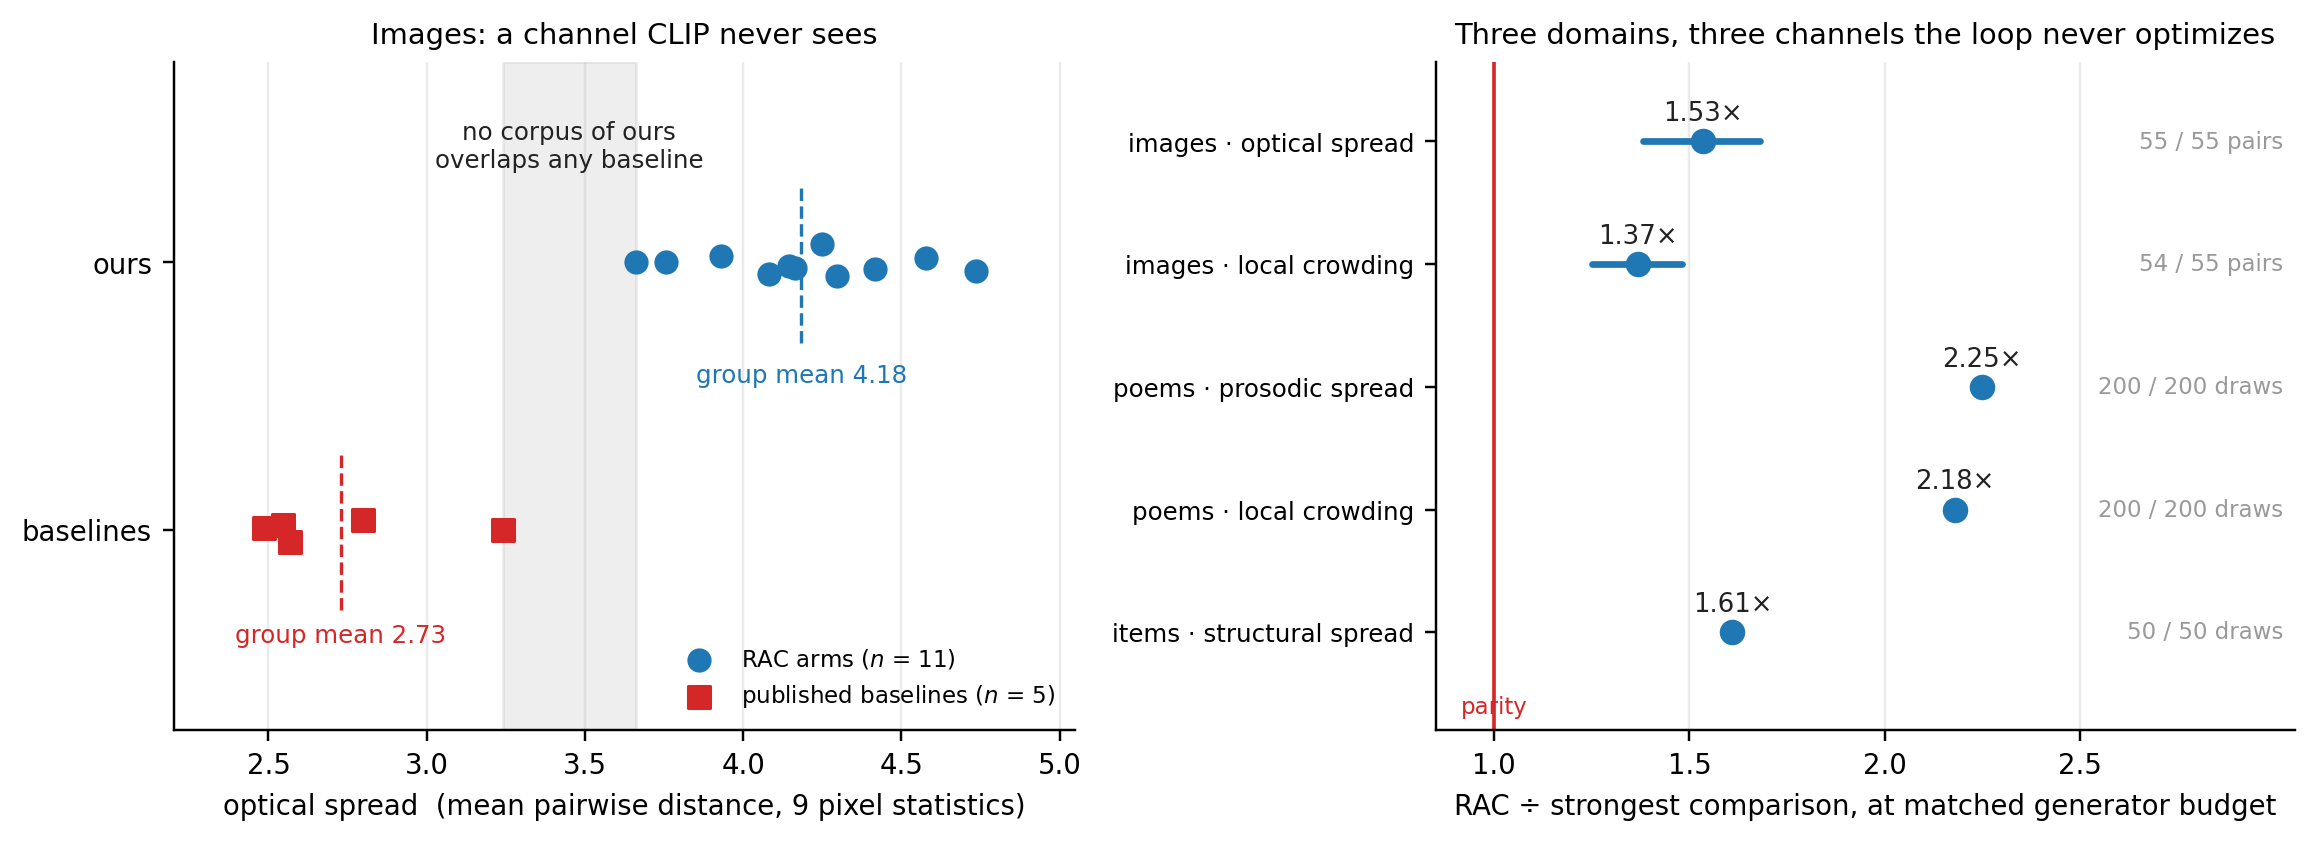
\includegraphics[keepaspectratio,alt={Figure 1. Separation measured outside the objective. Left: every image corpus at matched n = 60 on nine pixel statistics --- a channel with no connection to the CLIP or text embeddings the loop selects on. Every one of our eleven corpora exceeds every one of the five published baselines. Right: the same comparison in all three artifact domains, on the channel each domain\textquotesingle s objective cannot see, at matched generator budget; intervals are bootstrap 95\% CIs on the ratio of group means where the group sizes support them, and the annotation gives the number of resamples favouring RAC.}]{figures/fig22_out_of_objective.png}}

\emph{Figure 1. Separation measured outside the objective. Left: every
image corpus at matched n = 60 on nine pixel statistics --- a channel
with no connection to the CLIP or text embeddings the loop selects on.
Every one of our eleven corpora exceeds every one of the five published
baselines. Right: the same comparison in all three artifact domains, on
the channel each domain\textquotesingle s objective cannot see, at
matched generator budget; intervals are bootstrap 95\% CIs on the ratio
of group means where the group sizes support them, and the annotation
gives the number of resamples favouring RAC.}

\textbf{The objective has to be named before the number means anything.}
Corpus objectives fall into two classes --- \emph{covering} the
reachable space, and \emph{packing} it so no two items collide ---
usually spoken of interchangeably. They are not interchangeable, and
each class\textquotesingle s characteristic tool damages the
other\textquotesingle s score. Greedy \emph{k}-center, the classical
packing algorithm, wins min-gap in both of our domains and finishes last
on coverage, at a sixth of random selection. Orthogonalized
conditioning, the component that makes RAC work under packing,
\emph{reduces} coverage below plain conditioning when carried across,
and finishes last of the nine seeded arms. The two highest-Vendi
selectors we measure are the two worst covering ones (§3).

\textbf{Conditioning relocates a corpus\textquotesingle s repetition
unless it names the whole space the measure is defined over.} This is
the prescription we would keep if we could keep one. An axis enumerating
five of ten task categories moves an enormous amount of probability mass
onto those five and leaves total spread unchanged, because the five it
does not name are driven out; an axis enumerating all ten raises spread
in both a lumpy corpus and an already-flat one. The same rule holds one
level down, inside a single axis level, where a construct realized
through one lexical device is invisible to every realization audit in
the literature and to every diversity measure in this paper (§8.3).

Underneath all three is a single limit, made precise in §4: no selection
rule can outrun the conditional support of the generator it draws from,
so the only move that changes the asymptote is one that widens that
support.

\subsubsection{1.1 The oracle asymmetry}\label{11-the-oracle-asymmetry}

We assume throughout:

\begin{quote}
\textbf{Assumption (embedding oracle, no inverse).} We have access to
\emph{E}: Text → ℝ\(^{D}\), computable on demand. We have \textbf{no}
\emph{E}\(^{-1}\): ℝ\(^{D}\) → Text.
\end{quote}

This is the structural fact that shapes the entire design. Given a
corpus \emph{X\(_{n}\)} we can compute, exactly and cheaply, the point
in ℝ\(^{D}\) that would most improve any of our diversity measures ---
the direction of least occupied spectral energy, the centre of the
largest empty ball, the point maximizing marginal coverage. Knowing that
point is worth nothing on its own, because no procedure turns a target
embedding back into a poem.

Consequently the system cannot \emph{solve} for its next item. It can
only \textbf{propose} (sample from \emph{p}(· \textbar{} \emph{x}) for
some prompt \emph{x} we can write), \textbf{measure} (embed the
proposals and score them), and \textbf{select} (keep one). All of the
control is in the choice of \emph{x}, and that choice is expressible
only in language. This is why the latent variables here are
language-valued --- named axes with named levels --- rather than
continuous codes: they are the only handles that reach the generator. It
is also why the axis scoring of §5 exists. \textbf{The axis scoring is a
surrogate for the missing inverse}: unable to decode the direction we
want to travel, we score the language-valued conditions we \emph{can}
write by how nearly their induced output distributions point that way.

\subsubsection{1.2 Contributions}\label{12-contributions}

\begin{itemize}
\tightlist
\item
  \textbf{A generator loop that improves a chosen measure} (§5).
  Language-valued axes elicited from the generator, ranked by a scoring
  rule, with exhausted ones split recursively into conditional sub-axes.
  The measure enters at two points only, so pointing the loop at a
  different measure means changing those two and nothing else.
\item
  \textbf{A competitive result across five domains} (§7). Against five
  published methods at matched \emph{n}, RAC wins every metric in both
  text domains, beating the strongest baseline by 36\% in mean-centered
  Vendi at matched \emph{n} = 1,000; its exam bank contains no enemy
  pair at the judged radius, against 94.9\% usable for human-written
  MMLU and 15.3\% for naive prompting; and against released instruction
  corpora it places first of twelve at 0.4441 against
  Alpaca\textquotesingle s 0.3722.
\item
  \textbf{Separation on channels the method never optimizes} (§7.5), in
  all three artifact domains, at matched generator budget, with the most
  obvious confound removed in each case. These are the comparisons that
  cannot be a restatement of the selection rule, and they are the ones
  we would defend first.
\item
  \textbf{Evidence that the measure has to be named} (§3). Greedy
  \emph{k}-center wins min-gap in both domains and finishes last on
  coverage, and each measure\textquotesingle s characteristic tool
  damages the other\textquotesingle s score.
\item
  \textbf{A manipulation-based scoring rule for conditioning variables}
  (§5.3). The obvious observational estimator is not merely noisy but
  \emph{inverted}: it penalizes an axis in proportion to how well the
  axis works. On data where the answer is fixed by construction, the
  observational form ranks the inert axis first in 17 of 24 runs; the
  repair recovers the true order in 24 of 24.
\item
  \textbf{The completeness rule for conditioning} (§8.3), with the two
  audits that make it visible: realization has to be checked between
  levels \emph{and} within one, and an axis can be present, obeyed, and
  still realized the same way every time.
\item
  \textbf{A theory of what limits both objectives} (§4), with fifteen
  numerical checks.
\end{itemize}

\textbf{What is deferred to a companion paper.} Every measure here is
computed in an embedding, and in two of our domains that embedding is a
proxy for an artifact that lives elsewhere --- a rendered image, a
rendered instrumental. How large the gap between proxy and artifact is,
which embedder to steer through, how to close the loop in the
artifact\textquotesingle s own space, and what an embedding cannot see
at all are treated in \emph{Proxy Embeddings: Steering and Measuring
Diversity Through a Space That Is Not the Artifact\textquotesingle s},
which extends the method across that gap. Where this paper depends on
one of those results it says so and cites the section.

\subsection{2. Related work}\label{2-related-work}

\textbf{Synthetic instruction corpora.} Self-Instruct (Wang et al.,
2023) bootstraps instructions from a seed pool with few-shot exemplars
and a ROUGE-L similarity filter; the Stanford Alpaca corpus (Taori et
al., 2023; 52,002 items) is its canonical output. Evol-Instruct /
WizardLM (Xu et al., 2023) \emph{mutates} existing instructions with
depth and breadth operators, released as WizardLM\_evol\_instruct\_V2
(143,000 items). Persona-Hub (Ge et al., 2024) conditions on a catalogue
of \textasciitilde1B personas, releasing 50,000 persona-synthesized
instructions; it is the closest published relative of latent-axis
conditioning, differing in that its catalogue is mined at scale and
flat, where our axes are elicited from the generator and refined into a
tree. AttrPrompt (Yu et al., 2023) similarly conditions on attribute
dimensions. We compare against the \emph{released artifacts} of the
first three (§7.3) rather than against reimplementations, since a
reimplementation can be weak in ways that flatter us.

\textbf{Selection and subset choice.} Farthest-point traversal
(Gonzalez, 1985) 2-approximates \emph{k}-center, the packing objective;
SemDeDup (Abbas et al., 2023) removes semantic near-duplicates at a
fixed radius; determinantal point processes (Kulesza \& Taskar, 2012;
Chen et al., 2018) model repulsion via volume. All are \emph{post hoc}
selectors over a fixed pool, which is their limitation here: they cannot
change what is in the pool, and §4 shows the pool is the binding
constraint. We use all three as baselines.

\textbf{Submodular maximization and the packing/covering distinction.}
The (1 − 1/e) greedy guarantee for monotone submodular objectives is
Nemhauser, Wolsey \& Fisher (1978); hardness of beating it for
max-coverage is Feige (1998). Sieve-streaming (Badanidiyuru et al.,
2014) gives the single-pass regime our sequential setting approximates,
and facility location (Lin \& Bilmes, 2011) is the standard submodular
model of representativeness. \emph{k}-median/facility-location minimizes
\emph{average} service distance and behaves like our coverage objective
--- measure-weighted, bulk-first, outlier-indifferent --- where
\emph{k}-center does not; coreset constructions (Har-Peled \& Mazumdar,
2004) draw the same line. Our contribution is not new theory for these
objects but the identification of which one a corpus-construction
requirement actually is, and measurement of what optimizing the wrong
one costs (§3.4).

\textbf{Quality-diversity.} MAP-Elites (Mouret \& Clune, 2015) maintains
one elite per cell of a hand-designed behavior space. Our axis lattice
is a close relative with three differences that matter: the descriptors
are elicited from the generator rather than designed by us, the lattice
refines itself when a cell saturates, and allocation is
marginal-gain-driven rather than one-per-cell. §4.6 quantifies what the
fixed-grid choice costs at small ε.

\textbf{Diversity metrics.} The Vendi Score (Friedman \& Dieng, 2022) is
the exponential of the von Neumann entropy of a normalized similarity
matrix, interpretable as an effective number of distinct items; we use
it throughout, and §4.6 and §7.5 record two regimes in which it is the
wrong estimator. Repeated sampling from aligned models is well
documented to produce low lexical and semantic entropy relative to base
models; we take that as the empirical starting point. Red-teaming work
(Ganguli et al., 2022; Perez et al., 2022) documents exactly the
clustering-into-attack-families failure that motivates a coverage
objective for safety suites.

\subsection{3. Two objectives, and why the number needs one
named}\label{3-two-objectives-and-why-the-number-needs-one-named}

Covering and packing are routinely treated as two phrasings of one goal.
On real corpora they rank methods almost oppositely, and each
one\textquotesingle s characteristic tool costs the other measurably.
This section states both, measures the reversal, and draws the
consequence for the loop.

\subsubsection{3.1 Packing (max-min)}\label{31-packing-max-min}

Under an unbounded horizon the objective is a two-term score evaluated
against everything generated so far. Let \emph{E} be an embedding oracle
and \emph{X\(_{n}\)} = \{\emph{x}\(_{1}\), \ldots, \emph{x\(_{n}\)}\}
the corpus. For a candidate \emph{c},

\[
J_\lambda(c \mid X_n) \;=\; \lambda \cdot \underbrace{\frac{1}{n}\sum_{i=1}^{n}\lVert E(c) - E(x_i)\rVert}_{\text{anchor: keep it typical}} \;-\; (1-\lambda)\cdot \underbrace{\min_{i \le n} \lVert E(c) - E(x_i)\rVert}_{\text{repulsion: keep it new}}
\]

and we accept the candidate minimizing \emph{J}\(_{λ}\). The anchor
keeps generation on the manifold, the repulsion pushes away from what
exists. Both terms are cheap online: the anchor decomposes into
distance-to-centroid plus a candidate-independent constant, so ranking
by it is \emph{O}(\emph{D}) per candidate and \emph{O}(1) in \emph{n},
and the repulsion needs one nearest-neighbour query, bounded by
subsampling. Packing is the right question when a single collision is a
defect on its own --- two exam items testing the same rule are a
security failure whatever the rest of the bank looks like.

\subsubsection{3.2 Coverage}\label{32-coverage}

Fix an embedding map into ℝ\(^{D}\) (we use unit-normalized 768-d
embeddings) and a radius ε \textgreater{} 0. The generator, prompted in
whatever ways the pipeline can reach, induces a \emph{reachable
distribution} μ. Given a budget \emph{n}, choose \emph{S} =
\{\emph{x}\(_{1}\), \ldots, \emph{x\(_{n}\)}\} to maximize the covered
measure

\(F_{\mu,\varepsilon}(S) = \mu\!\left(\bigcup_{x \in S} B(x,\varepsilon)\right)\),

the probability that a fresh draw lands within ε of some chosen item.
Equivalently, \emph{S} should be an ε-net for as much of μ as the budget
allows. Coverage is the right question when the corpus stands for a
population, as an evaluation suite or a training set does. Three choices
are deliberate:

\begin{itemize}
\tightlist
\item
  \textbf{Coverage of the reachable space, not of ℝ\(^{D}\).} Balls in
  empty space cover volume but no behaviour. The denominator is stated
  next to every coverage number; where corpora built by different
  methods are compared it is a held-out human-written reference
  identical for all of them (§7.3).
\item
  \textbf{ε is a resolution parameter, not a nuisance.} Small ε asks for
  exemplars of fine distinctions, large ε for one exemplar per coarse
  region, and the ranking of methods changes with ε. Every result names
  its radius or range of radii.
\item
  \textbf{Quality is a constraint, not part of the objective.} An item
  that covers new territory but fails a quality bar is not an asset, so
  the judge gate rejects it regardless of gain.
\end{itemize}

\subsubsection{3.3 Where they coincide, and where they do
not}\label{33-where-they-coincide-and-where-they-do-not}

For a fixed ε, a \emph{maximal} ε-packing is automatically an
ε-covering: any uncovered point could have been added to the packing. We
confirm this numerically on 3,000 held-out human instructions --- at
every ε tested, the greedy maximal packing covers 100.0\% of the set,
and the classical sandwich \emph{N}\(_{cov}\)(ε) ≤
\emph{N}\(_{pack}\)(ε) ≤ \emph{N}\(_{cov}\)(ε/2) holds. Run to
maximality, max-min \emph{is} a covering algorithm.

That duality concerns the worst-case radius. The coverage that matters
for synthetic data is \textbf{measure-weighted}, and the two come apart
exactly when the measure is non-uniform, which it always is.
\emph{k}-center is driven by outliers: every isolated point sets the max
and so commands a centre, and at a budget far below what the space
needs, every such item is a ball spent covering ≈ 0 measure.
Measure-weighted coverage is driven by mass: a second exemplar in a
heavy mode can be worth more than a first exemplar of a negligible one,
and junk is worth nothing because μ puts almost nothing near it. The
true dual of measure-weighted coverage is fractional set cover, whose
primal is submodular; max-min is not.

What the duality still buys is calibration. Even where packing is the
wrong way to \emph{place} points it is the right way to choose the
\emph{scale}: ε*(\emph{n}), the radius at which a maximal packing of the
reference has exactly \emph{n} centres, is the largest resolution at
which \emph{n} items could in principle cover, and it is the radius we
calibrate to.

\subsubsection{3.4 The reversal,
measured}\label{34-the-reversal-measured}

A leakage-free selection benchmark isolates the contrast with no
generator in the loop: one shared candidate pool, budget matched at 700
and 1,896 generations, selector shown only an estimation half of the
reference and scored on a disjoint held-out half.

{\footnotesize
\begin{longtable}[]{@{}>{\raggedright\arraybackslash}p{\dimexpr 0.4305\linewidth-2\tabcolsep\relax}>{\raggedright\arraybackslash}p{\dimexpr 0.1808\linewidth-2\tabcolsep\relax}>{\raggedright\arraybackslash}p{\dimexpr 0.2140\linewidth-2\tabcolsep\relax}>{\raggedright\arraybackslash}p{\dimexpr 0.1747\linewidth-2\tabcolsep\relax}@{}}
\toprule\noalign{}
selector & DALL·E coverage & psychometric coverage & DALL·E min-gap \\
\midrule\noalign{}
\endhead
\bottomrule\noalign{}
\endlastfoot
coverage-greedy (ours) & \textbf{0.4829} & \textbf{0.3901} & 0.299 \\
coverage-stream (ours) & 0.4200 & 0.3785 & 0.283 \\
ROUGE-L filter (Self-Instruct) & 0.4629 & 0.3575 & 0.208 \\
SemDeDup & 0.4600 & 0.3575 & 0.336 \\
random & 0.4629 & 0.3533 & 0.198 \\
MAP-DPP greedy & 0.3829 & 0.0988 & 0.402 \\
\emph{k}-center (Gonzalez) & 0.4114 & 0.0557 & \textbf{0.491} \\
\end{longtable}}

\textbf{\emph{k}-center wins min-gap outright in both domains and
finishes last on coverage}, at 0.0557 against random\textquotesingle s
0.3533 in the psychometric domain --- a sixth of what picking at random
achieves. The two highest-Vendi selectors, \emph{k}-center and MAP-DPP,
are the two worst covering ones. A practitioner who reads "diversity"
off a Vendi score and deploys the selector that maximizes it gets a
corpus covering less of the space than random selection.

The same dissociation appears with the full generation loop in place,
and in the other direction. The configuration that applies the packing
side\textquotesingle s \emph{orthogonalized conditioning} to the
coverage objective finishes \textbf{last of the nine seeded arms} in
§7.3, below plain conditioning at matched evaluated \emph{n} (0.2102
against 0.2127) and by more at matched budget (0.2941 against 0.3147,
though those two arms kept 1,152 and 1,310 items and the estimator is
monotone in items, so part of that larger gap is corpus size).
Orthogonalization steers generation away from the occupied span, which
is away from the reference-dense core coverage is paid to fill. And the
winning coverage corpus has the \textbf{lowest} mean-centered Vendi of
any configuration in its cohort (62.1, density 1.69) --- it spends items
where the reference measure is, near-duplicates included, exactly as
facility location prescribes. A single "diversity score" would rank the
coverage winner last.

\subsubsection{3.5 Why the scoring rule has to
fork}\label{35-why-the-scoring-rule-has-to-fork}

Two of the loop\textquotesingle s factors invert between the classes,
and the rest do not.

{\footnotesize
\begin{longtable}[]{@{}>{\raggedright\arraybackslash}p{\dimexpr 0.3854\linewidth-2\tabcolsep\relax}>{\raggedright\arraybackslash}p{\dimexpr 0.3090\linewidth-2\tabcolsep\relax}>{\raggedright\arraybackslash}p{\dimexpr 0.3056\linewidth-2\tabcolsep\relax}@{}}
\toprule\noalign{}
& packing / max-min & covering / coverage \\
\midrule\noalign{}
\endhead
\bottomrule\noalign{}
\endlastfoot
the ask & no two items alike, in \emph{n} turns & reach as much as
possible, in \emph{n} turns \\
governed by & the closest pair & the bulk \\
submodular & no & yes, so greedy carries (1 − 1/e) \\
classical kin & \emph{k}-center & facility location \\
\textbf{spread(\emph{a})} & \textbf{min} distance between level
centroids & \textbf{measure-weighted mean} distance \\
\textbf{headroom(\emph{a})} & levels not yet \textbf{used} & measure not
yet \textbf{covered} \\
value selection & max-min subset of levels & greedy marginal gain over
levels \\
failure mode & chases outliers into off-manifold junk & leaves the
frontier empty \\
\end{longtable}}

The behavioural difference shows on a two-line test. Given an axis with
three tightly clustered common levels and one rare outlying level,
max-min value selection picks the outlier \textbf{first} and coverage
value selection picks a cluster centre first and the outlier second.
That is \emph{k}-center versus facility location reproduced inside the
axis scoring, and it is the mechanism behind the benchmark above.

\subsubsection{3.6 What both classes share, and what
follows}\label{36-what-both-classes-share-and-what-follows}

Both are bounded by the same thing, and neither optimizer can fix it.
Coverage of a reachable manifold and packing within one are both limited
by that manifold\textquotesingle s dimension, which is set by how far
the prompt can move the generator (§4). Both need the same typicality
constraint to be well-posed, since a novelty-seeking score can otherwise
be satisfied by output that has left the manifold. And both are read
through an embedder whose geometry can invert the result: we report a
cross-corpus comparison in which our worst corpus by every other measure
(19.8\% exact duplicates) scores the \emph{highest} coverage, because at
an ε in the 2nd percentile of reference distances the metric rewards
centrality rather than spread.

Five practices follow, and we use them throughout.

\begin{enumerate}
\def\labelenumi{\arabic{enumi}.}
\tightlist
\item
  \textbf{Say which objective you mean.} They are different problems
  with different optimal policies, and "diverse" does not distinguish
  them.
\item
  \textbf{Count exact duplicates before computing anything.} A 74\%
  duplicate rate makes every distance statistic a statistic about
  duplication.
\item
  \textbf{Publish the pairwise-similarity distribution} your kernel
  operates on. Mean pairwise cosine was 0.883 in one of our corpora and
  0.444 in another under the same embedder; an ε or a Vendi score means
  nothing without it.
\item
  \textbf{Measure at the level of the artifact you ship.} Text-embedding
  similarity explains 14.5\% of the variance in whether rendered images
  look alike, pooled across seven rendered arms, and 8.2\% within-arm
  (§7.7; companion §4.2).
\item
  \textbf{Audit in a channel the objective never optimizes} (§7.5,
  §8.3). It is the only measurement in this paper that cannot be a
  restatement of the selection rule, and it is where both the strongest
  positive result and the largest undetected defect were found.
\end{enumerate}

\subsection{4. What limits both: the conditional
slice}\label{4-what-limits-both-the-conditional-slice}

Nothing in this section depends on which measure was chosen. The results
bound what a fixed prompt can reach at all, and a measure computed on
the resulting corpus inherits that bound whatever it is measuring. The
first group concerns the conditional support and applies to any
selection rule; the second concerns the covering functional in
particular, and is what makes greedy selection defensible when coverage
is the measure. Every claim is checked numerically; §4.6 reports the
checks, all fifteen of which are reproducible from the released code.

\subsubsection{4.1 The reachable manifold and the conditional
slice}\label{41-the-reachable-manifold-and-the-conditional-slice}

Let \emph{M} ⊂ ℝ\(^{D}\) be the reachable semantic manifold, dim
\emph{M} = \emph{d}: the embeddings of texts the generator could produce
under \emph{some} prompt. For a fixed prompt \emph{x}, let
\emph{S\(_{x}\)} ⊆ \emph{M} be the support of
\emph{E}\(_{\#}\)\emph{p}(· \textbar{} \emph{x}), with dim
\emph{S\(_{x}\)} = \emph{m}. The empirical claim behind everything below
is that \textbf{\emph{m} ≪ \emph{d}}. A prompt fixes topic, stance,
form, register and rhetorical strategy; what remains free is a
low-dimensional residue. Our live pilot supports this directly: sixty
poems from an identical naive prompt have a median nearest-neighbour
cosine similarity of 0.911 and a Vendi Score of 2.55 --- sixty samples
behaving like two and a half distinct items. We write \emph{g\(_{n}\)}
for the min-gap of a fresh draw against a corpus of size \emph{n}.

\subsubsection{4.2 Saturation, and why oversampling is not a
strategy}\label{42-saturation-and-why-oversampling-is-not-a-strategy}

\begin{quote}
\textbf{Theorem 1.} Let \emph{X\(_{n}\)} be \emph{n} i.i.d. draws from a
distribution with density bounded above and below on an
\emph{m}-dimensional manifold \emph{S}. For a fresh draw \emph{c} from
the same distribution, 𝔼{[}\emph{g\(_{n}\)}{]} = Θ(\emph{n}\(^{-1/m}\)).
\end{quote}

\emph{Proof sketch.} ℙ(\emph{g\(_{n}\)} \textgreater{} \emph{r}) = (1 −
μ(\emph{B}(\emph{c}, \emph{r})))\(^{n}\) and μ(\emph{B}(\emph{c},
\emph{r})) = Θ(\emph{r}\(^{m}\)) by density bounds on an
\emph{m}-manifold, so ℙ(\emph{g\(_{n}\)} \textgreater{} \emph{r}) ≈
exp(−\emph{n}Θ(\emph{r\(^{m}\)})), which transitions at \emph{r} =
Θ(\emph{n}\(^{-1/m}\)); integrating the tail gives the expectation. ∎

The content is the exponent. With \emph{d} = 32 a naive reading predicts
\emph{n}\(^{-1/32}\) --- essentially flat, novelty never exhausted. The
true rate at \emph{m} = 3 is \emph{n}\(^{-1/3}\), roughly a tenfold loss
of headroom per thousandfold of corpus. Measured slopes: −0.472
(\emph{m} = 2), −0.309 (\emph{m} = 3), −0.195 (\emph{m} = 5), against
−0.5, −0.333, −0.2.

\begin{quote}
\textbf{Corollary 1.1 (oversampling is not a strategy).} Drawing
\emph{K} candidates and keeping the most novel multiplies the expected
gap by Θ(\emph{K}\(^{1/m}\)) at best. To recover the headroom lost by a
1000× larger corpus, \emph{K} must grow by 1000.
\end{quote}

Verified at \emph{m} = 3: best-of-8 yields 2.19 against
\emph{K}\(^{1/3}\) = 2.00. Selection is a constant-factor fix to an
asymptotic problem. §8.4 measures what this ceiling looks like in a live
loop, and finds that a system can fail to reach even it by pointing its
selector somewhere else.

\begin{quote}
\textbf{Theorem 2 (the slice deficit).} If \emph{m} \textless{}
\emph{d}, then vol\(_{d}\)(\emph{S\(_{x}\)}) = 0, and the fraction of
\emph{M} within ε of \emph{S\(_{x}\)} is Θ(ε\(^{d-m}\)).
\end{quote}

\emph{Proof sketch.} The ε-neighbourhood of an \emph{m}-dimensional set
in \emph{d} dimensions is a tube of volume Θ(ε\(^{d-m}\)) ·
vol\(_{m}\)(\emph{S\(_{x}\)}) for ε below the reach of \emph{S\(_{x}\)};
divide by vol\(_{d}\)(\emph{M}). ∎

Measured at \emph{d} = 8, \emph{m} = 2: fitted exponent 5.06 against a
predicted 6, with covered fractions falling 0.051 → 0.0001 as ε goes 0.5
→ 0.12. The practical reading is severe. \textbf{A single prompt,
sampled infinitely often, covers essentially none of what the model
could write} --- not "less than we would like", but a fraction going to
zero polynomially as the resolution of interest sharpens.

\pandocbounded{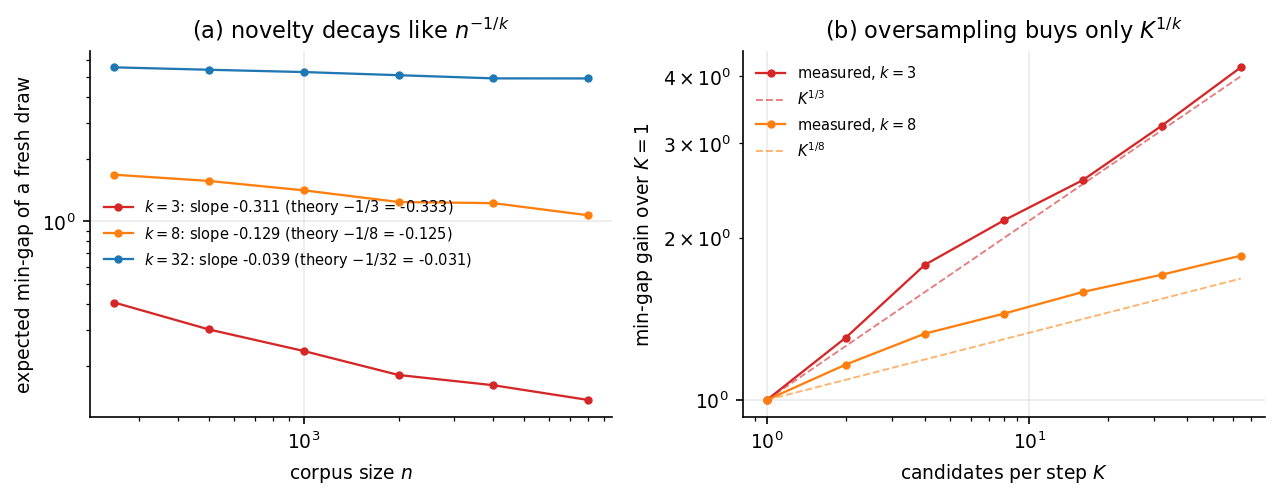
\includegraphics[keepaspectratio,alt={Figure 2. Measured saturation. (a) The expected min-gap of a fresh draw decays as n\^{}\{-1/m\} in the conditional dimension, with fitted slopes matching theory at m = 3, 8, 32. (b) Best-of-K oversampling buys only K\^{}\{1/m\}: at the conditional dimensions we measure, quadrupling the candidate pool buys tens of percent, not multiples.}]{figures/fig5_scaling.png}}

\emph{Figure 2. Measured saturation. (a) The expected min-gap of a fresh
draw decays as n\^{}(−1/m) in the conditional dimension, with fitted
slopes matching theory at m = 3, 8, 32. (b) Best-of-K oversampling buys
only K\^{}(1/m): at the conditional dimensions we measure, quadrupling
the candidate pool buys tens of percent, not multiples.}

\subsubsection{4.3 Transversality: which prompt motion
helps}\label{43-transversality-which-prompt-motion-helps}

Let a prompt schedule induce slices \emph{S}\(_{1}\), \ldots,
\emph{S\(_{P}\)}.

\begin{quote}
\textbf{Theorem 3.}
\(\dim\!\left(\bigcup_j S_j\right) = \min\!\left(d,\; m + \operatorname{rank}\{c_j - c_1\}\right)\),
where \(c_j\) is the centre of \(S_j\). In particular, displacements
lying inside \(\operatorname{span}(S_1)\) contribute nothing to the
union\textquotesingle s dimension.
\end{quote}

\emph{Proof sketch.} The union lies in the affine hull of the slice
frame plus the span of the centre displacements; dimensions add up to
that cap, and a displacement already inside the slice\textquotesingle s
own span adds no new direction. ∎

Measured via the participation ratio of the union\textquotesingle s
covariance spectrum: parallel displacements give effective dimension
1.88 --- the slices lie on top of each other at \emph{m} = 2 --- and
transverse displacements 11.18. This is the theorem that makes the axis
scoring of §5 possible: it turns "how much does conditioning on this
variable buy" into \textbf{how much of its variation lies outside what
the corpus already spans}, which is computable, where "how different
does it sound" is not.

\begin{quote}
\textbf{Theorem 4 (breadth versus depth).} Given budget \emph{B} split
as \emph{P} prompts × \emph{n} samples, with per-prompt switching cost
\emph{c} so that \emph{B} = \emph{P}(\emph{c} + \emph{n}): with \emph{c}
= 0 the coverage-optimal depth is \emph{n}* = 1, and for \emph{c}
\textgreater{} 0 the optimum is interior and increases with \emph{c}.
\end{quote}

Measured: with free switching, depth 1 achieves coverage 0.995 while
spending the whole budget on one prompt achieves 0.091, a 10.9×
difference; with \emph{c} = 3, \emph{n}* = 10; with \emph{c} = 30,
\emph{n}* = 30. \textbf{The ratio of prompt-switching cost to sampling
cost sets the batch size, and nothing else does.} Our pipelines sit near
the cheap-switching regime --- in the live pilot we measure \emph{c} ≈
0.10 generation-equivalents --- which is why every policy here draws its
\emph{K} candidates from \emph{K} fresh specs rather than sampling any
spec deeply.

For the packing objective this leaves the two terms of \emph{J}\(_{λ}\)
cheap and the candidate set expensive. Writing μ\(_{n}\) for the corpus
centroid,
\(\frac{1}{n}\sum_i \lVert c - x_i\rVert^2 = \lVert c - \mu_n\rVert^2 + \frac{1}{n}\sum_i \lVert x_i - \mu_n\rVert^2\)
(verified to zero relative error), and the second term does not depend
on \emph{c}, so ranking by mean squared distance to the corpus is
ranking by distance to the centroid --- \emph{O}(\emph{D}) per
candidate, \emph{O}(1) in \emph{n}. \textbf{The bottleneck is that both
terms are evaluated on candidates drawn from an \emph{m}-dimensional
slice.}

\subsubsection{4.4 Coverage: submodularity, greedy, and the streaming
case}\label{44-coverage-submodularity-greedy-and-the-streaming-case}

For any measure μ and radius ε,
\(F(S) = \mu(\bigcup_{x \in S} B(x,\varepsilon))\) is monotone (adding a
ball cannot uncover anything) and submodular: the marginal gain of \(x\)
given \(S\) is
\(\mu(B(x,\varepsilon) \setminus \bigcup_{y \in S} B(y,\varepsilon))\),
and since \(S \subseteq T\) implies
\(\bigcup_S B(y,\varepsilon) \subseteq \bigcup_T B(y,\varepsilon)\), the
set being subtracted only grows. Nothing about balls is essential ---
any map from items to measurable footprints gives a submodular \emph{F}.
The same argument applies verbatim to the Monte-Carlo estimator we
optimize: with a reference pool \emph{P}, item \emph{x} covers the fixed
subset \(N_\varepsilon(x) = \{p : \lVert p - x\rVert \le \varepsilon\}\)
and \(\hat F(S) = |\bigcup_{x \in S} N_\varepsilon(x)|/P\) is a finite
coverage function, monotone submodular exactly, at every sample of the
pool. Greedy therefore satisfies
\(\hat F(S_{\text{greedy}}) \ge (1 - 1/e) \cdot \max_{|S| \le n} \hat F(S)\),
tight for the class (Feige, 1998).

A generation pipeline cannot pick from a precomputed ground set:
candidates arrive \emph{K} at a time and must be accepted or discarded
immediately. Our per-step rule --- take the best of \emph{K} fresh
candidates by marginal gain --- is the natural best-of-\emph{K}
relaxation of sieve-streaming: weaker in the worst case, stronger on
exchangeable streams like ours, where each batch is i.i.d. from the
current proposal distribution and thresholding would only discard
budget. What matters for scaling is that the marginal-gain oracle is
\emph{O}(\emph{K} · \emph{P}) per step against a fixed-size pool with an
incrementally maintained covered mask --- \emph{O}(1) in \emph{n}.

Estimation error is Hoeffding: a 95\% band of
\(t_{95} = \sqrt{\ln(2/0.05)/(2P)}\), about ±0.030 at \emph{P} = 2,000
and ±0.015 at \emph{P} = 8,000. That bound is for \emph{fixed S}; a set
selected by optimizing \(\hat F\) on the same pool is biased upward on
that pool, which is why every coverage number reported here is computed
on held-out material the selector never saw.

\subsubsection{4.5 The reachability gap: conditioning, not selection, is
where the coverage
is}\label{45-the-reachability-gap-conditioning-not-selection-is-where-the-coverage-is}

The single most consequential simulation is the one that separates the
two levers. Identical greedy selection (ε = 1.0, \emph{k} = 300,
\textbar ground\textbar{} = 2,000) is run against three proposal
distributions and scored on one held-out full-mixture pool. An
\textbf{oracle} ground set drawn from the full latent mixture --- the
best a selector could do if conditioning reached everything --- covers
0.387. A \textbf{proposal-limited} ground set drawn from the base specs,
which reach 25 of 60 modes, covers 0.212. That 17.4-point gap is one no
selection algorithm can close, because the deficit is in what the
generator can be made to emit. A \textbf{refined-proposal} ground set,
one spec per mode, covers 0.374 and recovers 92.5\% of it.

Two corollaries of the same experiment sharpen what "widening the
support" means. \textbf{Lattice size is not reachable dimension}: two
worlds with identical lattice size (1,024 distinct specs) but different
rank of the level-direction span cover their own reachable pools at
49.0\% (rank 10) against 68.1\% (rank 2) --- the number of distinct
prompts you can write says nothing about how much there is to cover, and
a huge lattice over low-rank level directions is a thin space wearing a
combinatorial costume. And \textbf{refinement pays only if the children
move}: tight children at 0.25× displacement produce draws that are
36.7\% already covered by the pre-refinement corpus and add +0.02
effective dimensions --- almost pure density --- where full-length
isotropic displacement produces 0\% pre-covered draws and +0.13, and
transversality-guided displacement 0\% and +0.14. Splitting a saturated
cell into tighter sub-levels is worth its cost only when the split
displaces.

\subsubsection{4.6 Numerical
verification}\label{46-numerical-verification}

Each claim is checked against a numerical experiment designed to break
it.

{\footnotesize
\begin{longtable}[]{@{}>{\raggedright\arraybackslash}p{\dimexpr 0.5276\linewidth-2\tabcolsep\relax}>{\raggedright\arraybackslash}p{\dimexpr 0.4724\linewidth-2\tabcolsep\relax}@{}}
\toprule\noalign{}
check & result \\
\midrule\noalign{}
\endhead
\bottomrule\noalign{}
\endlastfoot
submodularity, exactly (5,000 nested chains, 200 candidates, 5,000-point
pool) & 0 violations of diminishing returns, 0 of monotonicity \\
greedy against \emph{exact} optima (10 instances, 142,506 subsets
enumerated each) & greedy/OPT = 1.0 on all ten; the 0.632 bound never
approached \\
Monte-Carlo band (200 pools per size against a 200k ground truth) &
95th-pctile error 0.042 / 0.020 / 0.011 at \emph{P} = 500 / 2,000 /
8,000 against Hoeffding 0.061 / 0.030 / 0.015 \\
saturation exponent (Theorem 1) & −0.472 / −0.309 / −0.195 against −0.5
/ −0.333 / −0.2 \\
best-of-\emph{K} return (Corollary 1.1) & 2.19 against
\emph{K}\(^{1/3}\) = 2.00 \\
slice deficit exponent (Theorem 2) & 5.06 against 6 \\
union dimension, parallel vs transverse (Theorem 3) & 1.88 against
11.18 \\
optimal depth vs switch cost (Theorem 4) & \emph{n}* = 1 / 10 / 30 at
\emph{c} = 0 / 3 / 30 \\
packing as a coverage algorithm (2,000 candidates, \emph{k} = 300,
held-out 20k pool) & full greedy 0.528, stream greedy (\emph{K} = 4)
0.484, random 0.420, max-min 0.143 \\
reachability gap (Proposition 1) & oracle 0.387, proposal-limited 0.212,
refined 0.374 \\
\end{longtable}}

Two of these carry more than confirmation. The packing row is the
pure-form double dissociation of §3.4 with no generator in the loop:
max-min is catastrophic \emph{as a coverage algorithm}, three times
below random, while being unbeatable at its own metric --- and stream
greedy at \emph{K} = 4 keeps 92\% of full greedy\textquotesingle s
coverage, which is what licenses the online form.

The allocation experiment adds a failure mode the clean theory hides.
Allocating \emph{n} = 10,000 items across 60 cells of known measure,
greedy marginal coverage beats the best closed-form rule by 7 points at
the radius it optimizes (0.618 against 0.547 for
proportional-to-measure) --- water-filling implemented empirically. At a
radius four times smaller it collapses to 0.004, because it saturated
its own pool after half the budget, its marginal signal went identically
to zero, and argmax tie-breaking dumped 5,083 of 10,000 items into one
arbitrary cell. \textbf{Greedy\textquotesingle s guarantee says nothing
about what it does after it has won.} At a finite budget, select at the
smallest ε you care about, or hand the post-saturation residual to an
explicit rule, or lower ε adaptively as gains vanish.

\subsection{5. Method: Recursive Axis
Conditioning}\label{5-method-recursive-axis-conditioning}

The loop is written once and pointed at a measure. The generator is
asked for the language-valued axes along which its own outputs can
differ, those axes are ranked and their most-different levels chosen,
and an axis that runs out of transverse variation is split into finer
conditional sub-axes. Two components read the measure and the rest do
not, which is what lets one stack serve objectives whose optima
conflict. The recursion is what the name refers to, and it is the part
that changes the asymptote rather than the constant.

\pandocbounded{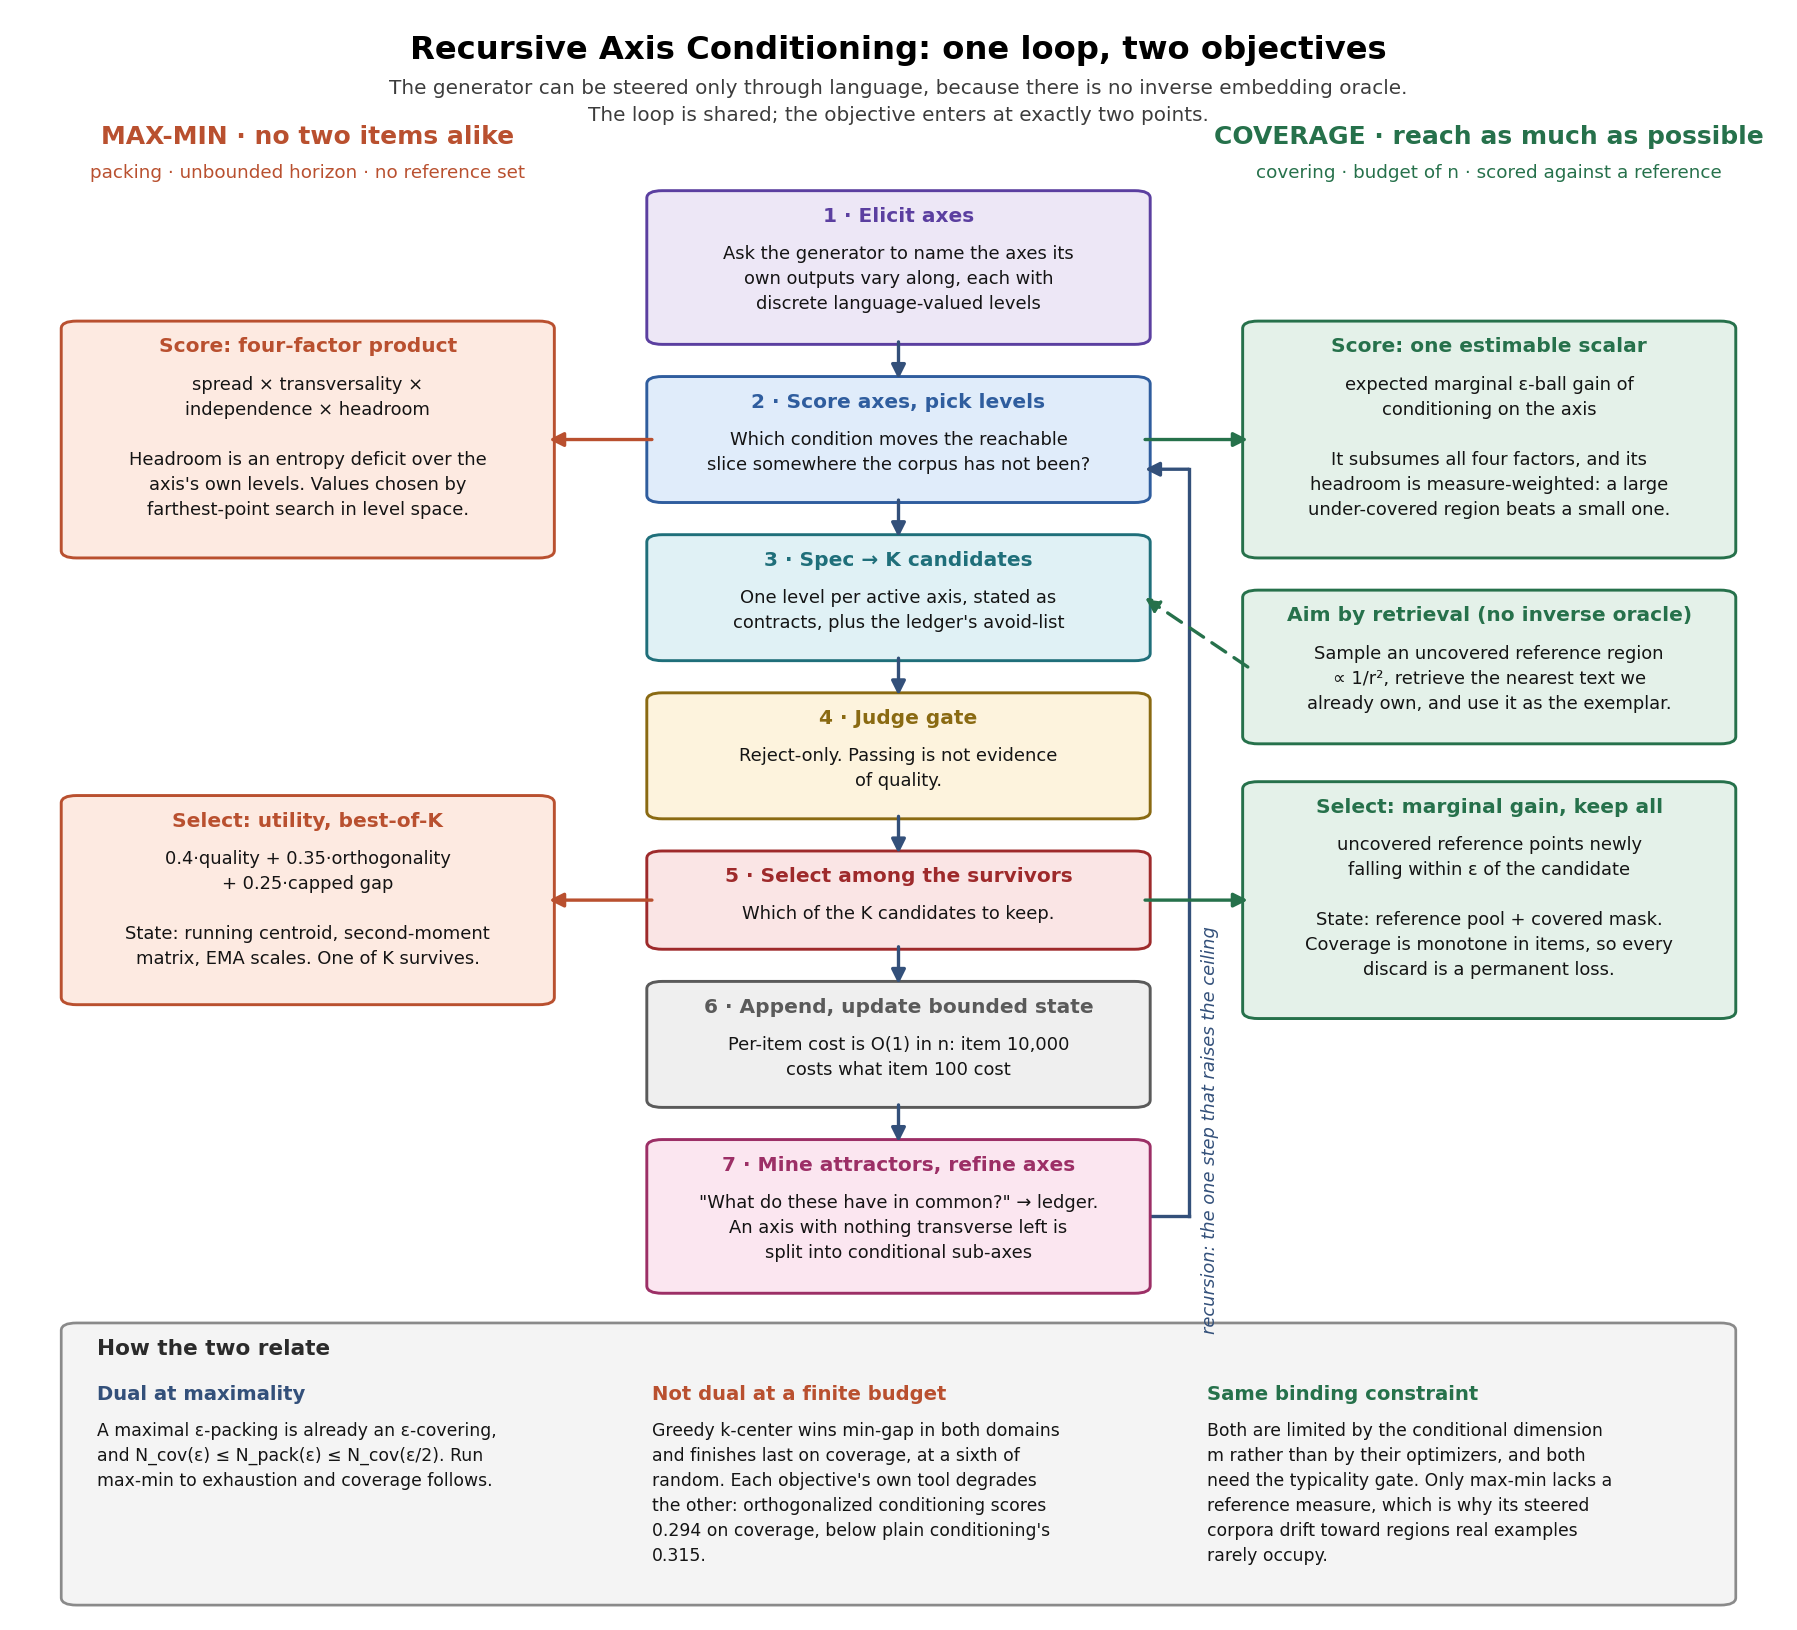
\includegraphics[keepaspectratio,alt={Figure 3. Recursive Axis Conditioning. The seven boxes down the centre run once per accepted item and are shared whatever the measure. The measure enters at two points only: how a candidate axis is scored (blue) and how one of the K candidates is chosen (crimson). Orange boxes are the packing instantiation of those two, green the covering one. Coverage adds one step packing has no use for --- aim by retrieval --- because only coverage has a reference distribution to aim at.}]{figures/fig15_rac_diagram.png}}

\emph{Figure 3. Recursive Axis Conditioning. The seven boxes down the
centre run once per accepted item and are shared whatever the measure.
The measure enters at two points only: how a candidate axis is scored
(blue) and how one of the K candidates is chosen (crimson). Orange boxes
are the packing instantiation of those two, green the covering one.
Coverage adds one step packing has no use for --- aim by retrieval ---
because only coverage has a reference distribution to aim at.}

\subsubsection{5.1 The stack}\label{51-the-stack}

Before any item is generated, the generator is asked to name the
dimensions along which its own outputs in this domain could differ, each
with a small set of discrete language-valued levels. For instrumental
music it returned \emph{formal trajectory}, \emph{timbral centre of
gravity} and \emph{pulse relationship}; for poetry, \emph{temporal
stance} and \emph{the register the poem refuses}. These names are the
entire steering vocabulary, because they are the only thing that can be
written into a prompt. Then, per accepted item, a bounded number of
model calls regardless of corpus size:

\begin{enumerate}
\def\labelenumi{\arabic{enumi}.}
\tightlist
\item
  \textbf{Spec choice.} Sample a pool of specs from the current axis
  lattice, embed their descriptions, keep the one with the largest
  residual outside the corpus\textquotesingle s occupied eigenspace.
  Orthogonalization at the level of \emph{conditions}, not outputs.
\item
  \textbf{Generation.} \emph{K} parallel completions conditioned on the
  spec, with the spec\textquotesingle s levels stated as
  \textbf{contracts} --- behaviours the text must exhibit, not
  suggestions --- plus an explicit avoid-list from the ledger.
\item
  \textbf{Judging.} One separate call scores craft (or, for exam items,
  validity) and checks each required behaviour. Generation never grades
  itself.
\item
  \textbf{Selection.} Utility = 0.4·quality + 0.35·orthogonality +
  0.25·capped gap, behind a typicality gate that hard-rejects candidates
  beyond \emph{z} running radii from the corpus centroid. The gate is
  negative supervision only --- it may reject, never endorse --- and the
  gap term is capped at two running scales, so no candidate earns
  unbounded credit for sitting far from everything.
\item
  \textbf{Mining.} Every 25 accepts, show the model 50 sampled items and
  ask what they have in common. Append the answer to a JSONL ledger; a
  bounded slice becomes the next prompts\textquotesingle{} avoid-list.
\item
  \textbf{Refinement.} On a saturation signal, ask the generator to
  split the dominant saturated cell.
\end{enumerate}

Every state the policy reads is bounded --- running centroid and second
moment, EMA scales, a fixed ledger slice, a recent window plus a bounded
random subsample of older items --- so the marginal cost of item 10,000
equals that of item 100.

\subsubsection{5.2 Scoring candidate axes: the four
factors}\label{52-scoring-candidate-axes-the-four-factors}

Theorem 3 says progress requires moving the prompt transversely to what
the corpus already spans; Theorem 4 says move often. Together they pose
a concrete question at every step: \textbf{among the latent variables we
could condition on next, which one moves the slice most transversely,
per unit of budget?} Having no inverse oracle, this is the closest
available substitute for computing the ideal next item. Each candidate
axis \emph{a} has language-valued levels; we embed the level
descriptions and read off four quantities.

\textbf{Spread} --- mean pairwise distance between
\emph{a}\textquotesingle s level embeddings. Are this
axis\textquotesingle s values actually different \emph{from each other}?
This catches the commonest failure of LLM-proposed axes:
plausible-sounding dimensions whose levels are near-synonyms.

\textbf{Transversality} --- the fraction of \emph{a}\textquotesingle s
level-to-level variation lying outside the corpus\textquotesingle s
occupied eigenspace (top eigenvectors carrying 80\% of spectral energy).
This is Theorem 3 made into a number. An axis whose levels differ only
along directions the corpus already spans adds density, not reach.

\textbf{Independence} --- 1 − max principal-angle cosine between
\emph{a}\textquotesingle s variation subspace and those of the axes
\textbf{already in use}. Measured against the active set and never
against rival candidates: two equally good candidates would otherwise
drive each other\textquotesingle s score to zero and rank below a
useless axis with no near-twin. Redundancy \emph{among} candidates is a
selection problem, handled by greedy selection that re-scores after
every pick.

\textbf{Headroom} --- a normalized entropy deficit of how unevenly the
corpus has sampled \emph{a}\textquotesingle s levels, plus the fraction
of levels never used. This is the only time-varying factor, and it is
what makes the ranking change as generation proceeds. An axis can be
excellent and already spent.

The \textbf{promise} of an axis is the product:

\[
\mathrm{promise}(a) = \mathrm{spread}(a)\cdot\mathrm{transversality}(a)\cdot\mathrm{independence}(a)\cdot\mathrm{headroom}(a)
\]

Multiplicative and deliberately so: an axis needs all four, and any one
at zero should zero the score rather than be averaged away. A
high-spread axis with zero transversality is a distinction without a
difference; a perfect axis with zero headroom is already spent. Cost is
\emph{O}(\textbar{}\emph{A}\textbar{} · \emph{D}²) per decision and does
not grow with \emph{n}.

\subsubsection{5.3 Scoring by manipulation, not
attribution}\label{53-scoring-by-manipulation-not-attribution}

All four factors are computed from \emph{level vectors}: one embedding
per level of each axis. In the text-only setting those are embeddings of
the level descriptions --- what a level \emph{claims} it will do. Once
the artifact can be embedded, the natural improvement is to replace them
with the centroid of everything actually produced under each level: what
the level \emph{did}. That substitution is what makes the scoring
empirical, and on its own it is wrong.

A centroid computed that way is a \textbf{marginal mean where the score
needs a partial effect}. Specs are sampled independently, so every other
axis varies inside each level group; with sixty items, seven axes and
five levels each, a group holds about twelve items whose spread is
mostly produced by the other six axes. The estimator cannot tell "this
axis moves the artifact" from "this axis co-occurred with movement", and
nothing in the loop ever intervenes on one axis while holding the rest
fixed.

The consequence is not a modest loss of precision. It is a
\textbf{systematic inversion}, and the mechanism is our own
transversality term. An axis that genuinely moves the artifact fills the
corpus with variance along its own direction; the occupied eigenspace
absorbs that direction; and transversality --- the fraction of an
axis\textquotesingle s variation lying \emph{outside} the occupied span
--- collapses toward zero for precisely that axis. An axis the generator
ignores contributes only isotropic noise, little of which the occupied
basis captures, so its transversality stays high. Because promise is
multiplicative, the effective axis sinks and the inert one rises.
\textbf{The better an axis is, the harder the score punishes it.}

A ground-truth test makes this exact. Construct three axes whose effects
are known by fiat: \textbf{A} displaces the output strongly along a
fixed direction, \textbf{C} weakly along another, and \textbf{B} does
nothing at all; sample specs independently, as the method samples them.
Over 24 seeds the attribution scoring ranks the \emph{inert} axis first
in 17 of 24 runs and the \emph{strongest} axis last in 16 of 24 (Figure
4, left). This is not noise around a correct answer; it is close to the
reverse of one.

The repair has three parts, and only the second changes the score.

\textbf{Partial effects.} Instead of a marginal centroid per level, fit
one additive model over all axes simultaneously --- effect-coded
indicators for every (axis, level) pair, ridge-regularized because
\emph{n} is small and the design is near-collinear whenever sampling is
uneven --- and read each axis\textquotesingle s level vectors off its
own coefficients. Effect coding rather than dummy coding, so no level is
silently privileged as a baseline.

\textbf{Realization.} Add a fifth factor: the share of corpus variance
the axis\textquotesingle s levels actually explain, with the null
expectation removed. Under exchangeable labels the between-group share
of variance has expectation (\emph{k}−1)/(\emph{n}−1) for \emph{k}
levels and \emph{n} items, per dimension and therefore for the sum over
dimensions, so the correction is analytic rather than a permutation loop
inside the generation path:

\[
\rho(a) = \max\left(0,\ \frac{\eta^2(a) - \frac{k-1}{n-1}}{1 - \frac{k-1}{n-1}}\right)
\]

and promise becomes the five-factor product, spread · transversality ·
independence · headroom · ρ.

Subtracting the null stops an axis scoring well merely for having many
levels and few observations. Realization is immune to the inversion
because it is measured on group structure rather than span geometry: an
axis with no effect has no between-level variance to find, whatever the
occupied basis is doing. And because promise is a product, an inert axis
now leaves the ranking instead of inheriting its
neighbours\textquotesingle{} variance. With this factor the strong axis
ranks first on all 24 seeds and the inert axis last on 19 of them; the
three separate cleanly on ρ itself, at 0.126, 0.006 and 0.001.

\textbf{Intervention.} When a generation budget can be spent on
measurement, the genuine \emph{do}-operator is available: hold a
background spec fixed, sweep a single axis across its levels, generate,
and pool the between-level variance over several backgrounds. Nothing
else moves, so no additivity assumption is needed. The cost is
\textbar levels\textbar{} × \textbar backgrounds\textbar{} generations
per axis, which is why this is a periodic probe on the few axes whose
observational realization is ambiguous rather than a per-item
computation. §8.1 reports what it finds in two domains.

\pandocbounded{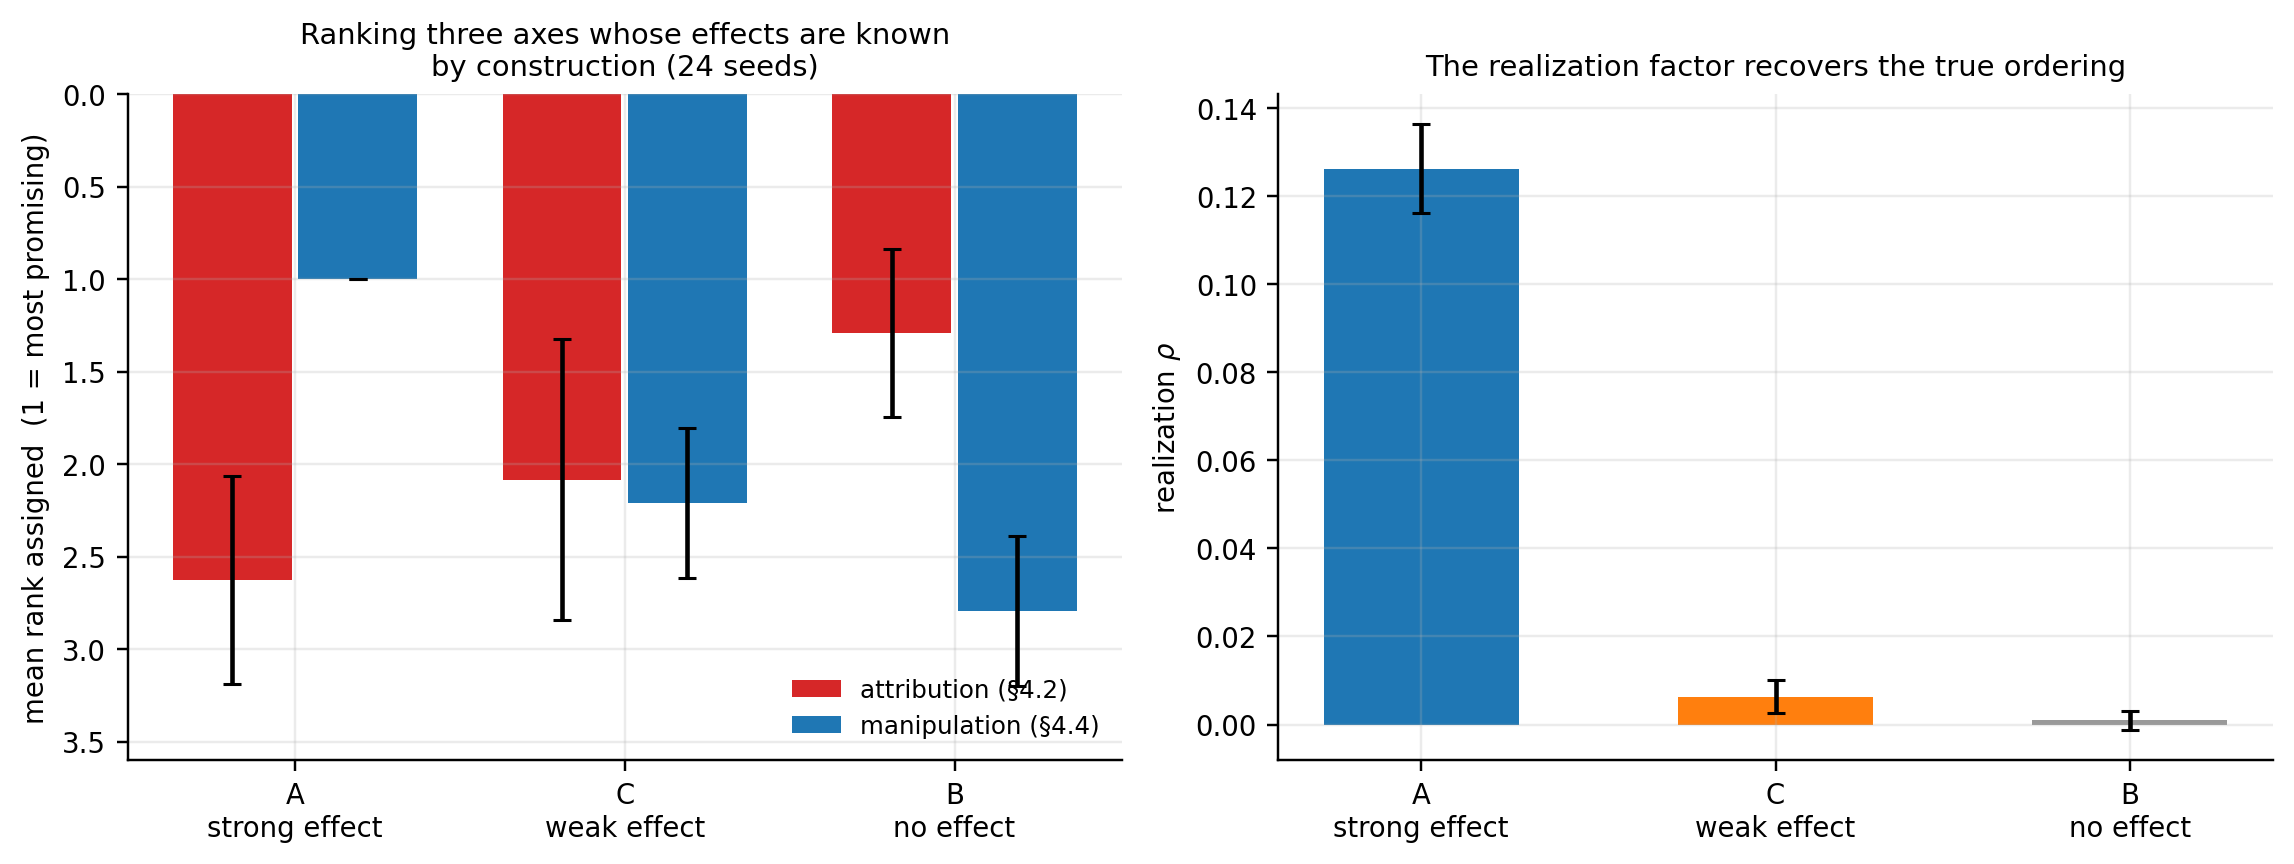
\includegraphics[keepaspectratio,alt={Figure 4. Left: mean rank assigned to three axes whose effects are known by construction, over 24 seeds. Attribution scoring ranks the inert axis B above the strong axis A; manipulation scoring recovers the true order. Right: the realization factor, which separates the three axes cleanly.}]{figures/fig18_scoring_inversion.png}}

\emph{Figure 4. Left: mean rank assigned to three axes whose effects are
known by construction, over 24 seeds. Attribution scoring ranks the
inert axis B above the strong axis A; manipulation scoring recovers the
true order. Right: the realization factor, which separates the three
axes cleanly.}

The practical stakes are highest at the \textbf{refine} signal, which
fires when no axis clears a promise floor. Under attribution an inert
axis retains enough borrowed variance to sit above the floor, so the
trigger stays shut and the system keeps conditioning on a dimension
nothing obeys. Realization sends such an axis to approximately zero,
which is the state the floor was written to detect. §8.1 shows this is
not a thought experiment: the axis this scoring ranked first in our own
published max-min image run is the one the image model was most
completely ignoring.

\subsubsection{5.4 Choosing values, recursing, and
expanding}\label{54-choosing-values-recursing-and-expanding}

Once an axis is chosen we do not sample its levels uniformly. Under
packing we take the \textbf{max-min subset} of its level embeddings by
greedy farthest-point search, seeded at the level furthest from the
level centroid --- the packing problem again, one level down. Under
coverage we take the greedy marginal-gain subset instead (§3.5).

When the best available promise falls below a floor, the scoring emits
\texttt{refine} instead of \texttt{condition}. This is the
\textbf{exhaustion signal}, and it is the honest one: it says the
current lattice has nothing transverse left to offer, and no amount of
further sampling will change that. The system then shows the generator
the saturated cell and the mined attractors and asks it either to split
a level into finer sub-levels or to mint a new axis that applies only
inside that cell. Refinement axes are \textbf{conditional} --- they
apply only when their parent level was chosen --- so the lattice is a
tree and refining a saturated region does not inflate cost elsewhere.

\textbf{Refinement is not expansion, and the difference bounds the
method.} Refinement fires on saturation, and saturation is evidence
\emph{from inside the lattice}: a cell stops producing mutually distant
items, so we subdivide it. Every axis that mechanism can reach is a
descendant of an axis the seed elicitation already proposed. It raises
resolution in directions the basis has; it cannot add a direction the
basis lacks. That limit is invisible to the trigger, because \textbf{a
dimension that is never sampled never saturates}. If the seed
elicitation returns seven axes belonging to one conceptual family ---
and it reliably does, since a single prompt asking for "independent axes
of variation" is itself a fixed prompt, subject to every argument in §4
--- then the corpus is bounded by the span of that family however deeply
any member is refined. Both of our domains fail exactly this way, along
family lines a practitioner would recognize on sight: the image axes are
all art-theoretic (appropriation, self-referentiality, seriality) and
none is optical; the poem axes are all rhetorical stance (temporal
stance, address geometry, claim posture) and none is prosodic.

The missing move is \textbf{expansion}: asking, from outside the
lattice, what the corpus does not vary. We add one step that does this
and nothing else. Periodically a judge is shown a sample of the
\emph{artifacts} --- the rendered images, or the poems themselves, never
their specs, so it cannot restate the axis set back to us --- together
with the list of axes already in use, and is asked to name the
dimensions along which the set does not vary and to return each as an
axis with concrete, verifiable levels. The new axes join the tree
through the same append-only path refinement uses. Two design choices
carry most of the weight. The judge is asked for \emph{absence}, which
is the opposite question from attractor mining --- mining names what the
corpus keeps doing so it can be repelled, expansion names what the
corpus never does so it can be reached. And the judge is told to stay
off the dimensions already present, because the failure mode of an
unconstrained "what is missing" prompt is a rephrasing of an axis
already in the set. The step costs two calls per run, and it is the only
mechanism here besides recursion that changes what is \emph{reachable}
rather than how efficiently the reachable is covered.

\subsubsection{5.5 The covering
instantiation}\label{55-the-covering-instantiation}

The covering instantiation is the same stack with the selection
objective and its bookkeeping swapped; we write RAC-coverage for it and
RAC-packing for the other. Four things change and one is added.

\textbf{The reachable pool becomes the denominator.} Before selection
begins, draw a pool of cheap unconditioned samples from the generator
and embed them. This pool \emph{is} the Monte-Carlo measure: coverage
means coverage of it. Cost is \emph{O}(\emph{P}) once, amortized over
the run.

\textbf{The four factors collapse into one.} Packing has no per-axis
marginal decomposition, because min-gap is a global property, so the
scoring must approximate "will this axis move the slice somewhere new"
from four geometric proxies. Submodular coverage has an exact marginal
quantity --- the expected marginal ε-ball gain of conditioning on the
axis, \(\mathbb{E}_{x \sim a}[F(S \cup \{x\}) - F(S)]\) --- and that one
scalar subsumes all four. An axis with near-synonym levels (no spread),
or whose slices sit inside covered territory (no transversality), or
which duplicates an axis already exploited (no independence, since the
covered mask already contains that axis\textquotesingle s contribution),
or whose region is already covered (no headroom) all have small expected
marginal gain. The headroom that remains is \emph{measure-weighted} by
construction: a large under-sampled region beats a small one because it
holds more uncovered pool mass. In practice we keep the embedding-based
spread and transversality and replace the entropy headroom with the
measure-weighted estimate.

\textbf{Selection becomes coverage-greedy.} Each step, embed the
\emph{K} candidates, compute each one\textquotesingle s marginal gain
--- the number of not-yet-covered pool points within ε\(_{sel}\) --- and
accept the gated candidate of maximum gain. The covered mask updates
incrementally, so per-step cost is \emph{O}(\emph{K} · \emph{P} +
\emph{P}) regardless of \emph{n}. \textbf{Coverage keeps every candidate
that clears the gate}, since covered measure only grows with items and a
discard cannot be undone.

\textbf{Refinement acquires an obligation.} Refinement changes the
reachable distribution, so the reference pool must be refreshed with
draws from the newly opened region, or the selector will see zero gain
precisely where the new territory is: its balls cover no \emph{old} pool
points.

\textbf{And one step is added: aim by retrieval.} Coverage is scored
against a reference distribution, so it can pick a specific
under-covered region to attack, sampling one in proportion to how sparse
it is. Having no inverse oracle it cannot turn that target point into
text; instead it retrieves the nearest text it already owns and hands
that to the generator as the exemplar to move toward or away from. The
target\textquotesingle s own \emph{k}-NN radius then selects the prompt
mode: a tight radius (dense region) asks the generator to imitate the
local task family closely, because a diversified item would land outside
the small ball it must hit; a wide radius (sparse region) asks for full
diversification, with the nearest own outputs shown as explicit
in-prompt negatives. §7.6 decomposes what each of those two modes
contributes.

\subsubsection{5.6 Why "orthogonalize", not
"randomize"}\label{56-why-orthogonalize-not-randomize}

Forcing randomness --- raising temperature, injecting random seed words
--- buys variance in the surface while leaving the mode structure
intact, and degrades quality monotonically because temperature cannot
distinguish \emph{surprising} from \emph{wrong}. The measurements bear
this out: raising sampling temperature to 1.6 moves distinct-2 from
0.3341 to 0.3342 and leaves 71.0\% of the corpus byte-identical
duplicates, against 73.6\% at the default. Forcing approximate
orthogonality asks a different question --- which direction is this
corpus not yet spending energy on --- which has a computable answer,
improves rather than degrades quality when paired with a quality term,
and stays informative as \emph{n} grows. "Be random" gets no harder to
satisfy and no more useful.

\subsection{6. Experimental setup}\label{6-experimental-setup}

\textbf{Generator and embedders.} \texttt{openai/gpt-5.6-luna} via
OpenRouter for generation, judging, attractor mining and axis
elicitation. Text embeddings: \texttt{nomic-embed-text} (768-d,
unit-normalized) served locally by Ollama, so embedding is free and the
loop is never rate-limited by its own measuring instrument. Images:
\texttt{gpt-image-1-mini}, embedded with CLIP ViT-B/32. Audio: Lyria 3
Pro instrumentals, embedded with CLAP and MERT. Every corpus is
append-only JSONL with embeddings checkpointed alongside, resumable
after a kill; every number carries a provenance tag naming the procedure
that produced it.

\textbf{Domains.} \emph{DALL·E instructions for post-modern artworks},
where diversity is the product and the same corpus can be measured in
three spaces --- words, text-embedding, and the rendered picture.
\emph{Psychometric test questions}, multiple-choice items assessing
general reasoning, where two items with the same construct are a
validity problem rather than an aesthetic one. \emph{Instruction
corpora}, for the head-to-head against released artifacts.
\emph{Poetry}, a pilot where craft rather than content carries the
variation. \emph{Instrumental-music prompts}, the longest chain in the
paper: latent axes → text prompt → two-minute instrumental → audio
embedding.

\textbf{Methods compared.} Five published approaches, implemented
faithfully rather than as strawmen, each getting the same generator,
embedder and budget accounting as ours.

{\footnotesize
\begin{longtable}[]{@{}>{\raggedright\arraybackslash}p{\dimexpr 0.4088\linewidth-2\tabcolsep\relax}>{\raggedright\arraybackslash}p{\dimexpr 0.5912\linewidth-2\tabcolsep\relax}@{}}
\toprule\noalign{}
arm & what it is \\
\midrule\noalign{}
\endhead
\bottomrule\noalign{}
\endlastfoot
\texttt{naive} & plain repeated prompting --- the honest floor \\
\texttt{high\_temp} & temperature 1.6 --- the trivial diversity lever \\
\texttt{self\_instruct} & \textbf{Self-Instruct / Alpaca}: few-shot
exemplars sampled from the pool, plus ROUGE-L ≤ 0.7 rejection against
it \\
\texttt{evol\_instruct} & \textbf{Evol-Instruct (WizardLM)}: sample an
existing item, apply a random evolution operator (deepen, concretize,
add constraint, harder reasoning, mutate form) \\
\texttt{persona} & \textbf{Persona-Hub / AttrPrompt}: a flat catalogue
of personas × attributes, sampled uniformly \\
\texttt{rac} & \textbf{Recursive Axis Conditioning} (ours) \\
\texttt{rac+vision} & RAC, plus steering on the \emph{rendered image}
(§7.7; companion §5.1) \\
\end{longtable}}

\texttt{persona} is the load-bearing comparison. It has language-valued
latent conditioning --- the same basic idea as ours --- but no
orthogonality selection, no ledger and no recursive refinement, so the
gap between \texttt{persona} and \texttt{rac} isolates what those three
components buy. One faithfulness caveat is deliberate:
Self-Instruct\textquotesingle s ROUGE filter compares a candidate
against the entire pool, which is \emph{O}(\emph{n})
longest-common-subsequence computations per candidate and comes to
dominate the loop at \emph{n} in the thousands, so we compare against a
bounded random sample of 120 pool members. That makes our
reimplementation \emph{weaker} than the original at large \emph{n}, and
the reason is itself a finding: the original\textquotesingle s
redundancy check does not have an infinite horizon, because its cost
grows linearly in the corpus it is protecting.

\textbf{What we measure, and what each measure misses.} We report
several because they disagree, and a corpus that one of them calls
healthy another calls collapsed.

\begin{itemize}
\tightlist
\item
  \textbf{Exact-duplicate rate} --- byte-identical repetition.
  Unambiguous, cheap, and the first thing to compute; blind to
  paraphrase.
\item
  \textbf{Distinct-\emph{n}, 4-gram self-repetition, \emph{n}-gram
  Vendi} --- surface statistics over token sequences. They catch
  templating that the duplicate rate misses and read meaning not at all.
  \textbf{These are independent of our objective}, since the method sees
  only embeddings and has no access to token counts or string identity.
\item
  \textbf{Mean-centered embedding Vendi} --- the exponential of the von
  Neumann entropy of the corpus Gram matrix, an effective number of
  distinct items. It summarizes the whole spectrum, which makes it
  insensitive to local structure. Centering matters as much as the
  statistic: the shared mean direction of text embeddings compresses the
  uncentered score by roughly 2.7×, so an uncentered Vendi reports the
  cone as much as the content.
\item
  \textbf{Median nearest-neighbour distance} --- how much room the
  typical item has. It goes to exactly zero when the median item has a
  perfect twin.
\item
  \textbf{Worst-case nearest-neighbour distance (the packing radius)}
  --- the only measure here under which a single collision is a defect
  regardless of everything else.
\item
  \textbf{Coverage, density, precision and recall against a reference}
  --- computed with reference-side \emph{k}-NN radii so nothing is
  tunable per corpus. These are the only measures that know what the
  space is supposed to look like, and the only ones that let corpora of
  different scales be compared. Covered fraction at a \emph{fixed}
  radius does not survive that comparison: it correlates −0.991 with
  within-corpus spacing, so it ranks corpora by how tightly they cluster
  rather than by how much they reach.
\item
  \textbf{A judged threshold}, where an application defines the failure
  (§7.4).
\item
  \textbf{Measures on the rendered artifact}, and \textbf{measures in a
  channel the loop never optimizes} (§7.5), which are the ones that
  cannot be circular.
\end{itemize}

Two facts about circularity are worth stating before the results. Our
packing selection rule maximizes a weighted sum of embedding-space
orthogonality and embedding-space min-gap, and we then report
embedding-space diversity metrics; centered Vendi is a monotone function
of how flat the Gram spectrum is, which is close to what the
orthogonality term climbs, and median nearest-neighbour distance
\emph{is} the min-gap term. Those wins should be read as confirmation
that the optimizer works, not as independent evidence. The independent
evidence is the literal measures, which the method never observes, and
the out-of-objective channels of §7.5, which live downstream of a
rendering step or in a feature space nothing in the loop touches. Sorted
by how much weight they can bear: embedding-space measures are partly
circular; literal-space measures are independent; rendered-artifact and
out-of-objective measures are the most independent, and they carry the
argument.

\textbf{Scale and cost.} The text corpora comprise 43,171 real
generations for roughly \$8.50 of OpenRouter spend, plus 1,796 rendered
images across sixteen image arms and up to three quality tiers, a
further 285 renders for the two render-side probes of §8, 100 rendered
Lyria instrumentals, and 236 adjudicated exam-item pairs. Both
\texttt{naive} arms reach \emph{n} = 10,000; the reimplemented baselines
reach 2,500 each. Every comparison is reported at a matched \emph{n}
that all compared arms actually reached. Total API spend across the
project is roughly \$40.

\subsection{7. Results}\label{7-results}

\subsubsection{7.1 Duplication under repeated
sampling}\label{71-duplication-under-repeated-sampling}

Two 10,000-item corpora, one call each, no selection:

{\footnotesize
\begin{longtable}[]{@{}>{\raggedright\arraybackslash}p{\dimexpr 0.3763\linewidth-2\tabcolsep\relax}>{\raggedright\arraybackslash}p{\dimexpr 0.1175\linewidth-2\tabcolsep\relax}>{\raggedright\arraybackslash}p{\dimexpr 0.1440\linewidth-2\tabcolsep\relax}>{\raggedright\arraybackslash}p{\dimexpr 0.1859\linewidth-2\tabcolsep\relax}>{\raggedright\arraybackslash}p{\dimexpr 0.1763\linewidth-2\tabcolsep\relax}@{}}
\toprule\noalign{}
domain & \emph{n} & unique texts & exact-duplicate rate & most-repeated
item \\
\midrule\noalign{}
\endhead
\bottomrule\noalign{}
\endlastfoot
DALL·E instructions & 10,000 & 10,000 & 0.000 & 1× \\
psychometric items & 10,000 & 2,645 & \textbf{0.736} &
\textbf{2,726×} \\
\end{longtable}}

In the psychometric domain 73.6\% of a ten-thousand-item corpus is exact
duplicate text and a single question accounts for 2,726 of them. The
four most frequent items are these:

{\footnotesize
\begin{longtable}[]{@{}>{\raggedright\arraybackslash}p{\dimexpr 0.4544\linewidth-2\tabcolsep\relax}>{\raggedright\arraybackslash}p{\dimexpr 0.5456\linewidth-2\tabcolsep\relax}@{}}
\toprule\noalign{}
copies & item \\
\midrule\noalign{}
\endhead
\bottomrule\noalign{}
\endlastfoot
2,726 & What number comes next in the sequence: 2, 6, 12, 20, 30, ? (A.
40 B. 42 C. 44 D. 46) \\
655 & What number \emph{should} come next in the sequence: 2, 6, 12, 20,
30, ? (A. 40 B. 42 C. 44 D. 46) \\
467 & What number comes next in the sequence: 2, 6, 12, 20, 30, ? (A. 36
B. 40 C. 42 D. 44) \\
434 & What number comes next in the sequence: 3, 8, 15, 24, 35, ? (A. 46
B. 48 C. 50 D. 52) \\
\end{longtable}}

Deduplication does not rescue this corpus: removing the 2,726 identical
copies leaves the three paraphrases behind, and a paraphrase of a live
item is an enemy item on any bank a psychometrician would sign off on.
No embedding, threshold or interpretation is required to see it.
Temperature barely helps --- at \emph{T} = 1.6 the duplicate rate is
still 0.710 --- and conditioning nearly eliminates it: persona
conditioning drops it to 0.009 and axis conditioning to 0.000. Between
those two numbers is the whole argument of §5.6: randomness does not buy
diversity, conditioning does. It also shows the failure is domain-shaped
and invisible from one vantage point. The identical pipeline, prompt
style and model produce zero duplicates on DALL·E instructions; a
practitioner who validated on the first domain and deployed on the
second would ship a bank that is three-quarters one question.

\textbf{The same failure is visible in a corpus with no duplicates at
all.} The poetry pilot has an exact-duplicate rate of 0.000 under naive
prompting and a distinct-2 of 0.610, so every literal counter reports a
healthy corpus. Here are the opening lines of eight poems sampled at
random from those sixty:

\begin{itemize}
\tightlist
\item
  \emph{At dawn, the river gathered up the stars}
\item
  \emph{At dusk, the windows gather fire}
\item
  \emph{At dusk, the rooftops gather amber light}
\item
  \emph{At dusk, the windows gather amber light}
\item
  \emph{At dawn, the windows gather up the rain}
\item
  \emph{At dusk, the river gathers every color}
\item
  \emph{At dusk, the river gathers up the day}
\item
  \emph{At dusk, the river gathers up the sky}
\end{itemize}

Eight of eight are the same sentence with two slots filled. The closest
pair sits at cosine similarity 0.946 and shares its first line verbatim
before diverging into the same sparrow stitching the same thread across
the same evening. Sixty samples from one prompt behave like two and a
half distinct items by Vendi Score, and the duplicate counter sees none
of it.

Eight openings from the sixty RAC produced under the same generator and
budget:

\begin{itemize}
\tightlist
\item
  \emph{Had you arrived at the registry after midnight, when the lamps
  were still accountable}
\item
  \emph{We have tried to piece that evening together from what
  remained.}
\item
  \emph{I am the conjurer in the green coat, stepping into the light.}
\item
  \emph{I have reconstructed the trench, Mara, from the surviving datum
  points.}
\item
  \emph{I wore the cobalt pressure suit, and the regolith took my
  weight}
\item
  \emph{We went back through that winter in our minds.}
\item
  \emph{"Attend, O citizens, beneath the unappeased sky:}
\item
  \emph{At the appointed hour, you will rise beneath the bells}
\end{itemize}

Counterfactual conditional, collective reconstruction, first-person
performance, a report addressed to a named absent person, plain
retrospect, public proclamation, prophecy. The closest pair RAC produces
sits at 0.809 and shares a subject rather than a template. The
measurements follow the reading: RAC holds 2.7× the median
nearest-neighbour distance (0.239 against 0.089) and cuts 4-gram
self-repetition by a factor of 37 (0.0023 against 0.0855) at a
distinct-2 of 0.774 against 0.610. Mean-centered Vendi moves very little
in comparison, 38.81 against 37.00, and that is the right reading of it:
a spectral summary of sixty points in 768 dimensions is close to
insensitive to the difference between sixty poems that begin the same
way and sixty that do not. The nearest-neighbour statistic registers it,
and the page registers it immediately.

The exam domain shows the same contrast at the level of what an item
asks. One representative item from each of four methods, same generator,
same budget:

\begin{itemize}
\tightlist
\item
  \textbf{naive} --- \emph{What number comes next in the sequence: 2, 6,
  12, 20, 30, ? (A. 40 B. 42 C. 44 D. 46)}, generated 2,726 times.
\item
  \textbf{Self-Instruct} --- \emph{What number should come next in the
  sequence? 3, 8, 15, 24, \_\_\_ (A. 32 B. 35 C. 36 D. 39)}. The ROUGE
  filter blocks the byte-identical copy and admits the same item on new
  numbers.
\item
  \textbf{persona conditioning} --- \emph{Of 120 rare books examined, 70
  contain a particular watermark, 50 have documented provenance, and 30
  have both. How many have neither?} A costume --- rare-book forgery,
  flood-risk pricing, restaurant scheduling --- is drawn over a
  recurring set-arithmetic skeleton.
\item
  \textbf{RAC} --- \emph{An incident report recorded the following
  events. The pump had to be primed before the valve could be opened.
  The technician was using a blue clipboard, and rain was visible
  outside. The heater could be switched on only after the valve was
  opened\ldots{} printing the label was independent of the
  pump-and-heater process. Which sequence of events is consistent with
  the report?}
\end{itemize}

The variation is in the cognitive operation being assessed and in how
the wrong answers are built rather than in the surface story. That is
the axis structure showing through: two items wearing different costumes
over one rule are still enemy items, and two items testing different
operations are not, however similar they read. One cost is visible in
the same examples --- RAC items carry deliberate irrelevant detail,
which the \emph{distractor logic} axis asks for and real psychometric
items use, and it makes them long; the RAC exam corpus reached 1,999
items on the budget that returned 10,000 naive ones.

\textbf{Literal and latent diversity move in opposite directions}, which
is why both are reported throughout. Measuring the DALL·E naive corpus
as it grows:

{\footnotesize
\begin{longtable}[]{@{}>{\raggedright\arraybackslash}p{\dimexpr 0.3186\linewidth-2\tabcolsep\relax}>{\raggedright\arraybackslash}p{\dimexpr 0.1259\linewidth-2\tabcolsep\relax}>{\raggedright\arraybackslash}p{\dimexpr 0.1868\linewidth-2\tabcolsep\relax}>{\raggedright\arraybackslash}p{\dimexpr 0.1736\linewidth-2\tabcolsep\relax}>{\raggedright\arraybackslash}p{\dimexpr 0.1951\linewidth-2\tabcolsep\relax}@{}}
\toprule\noalign{}
\emph{n} & distinct-2 & 4-gram self-repetition & \emph{n}-gram Vendi &
centered embedding Vendi \\
\midrule\noalign{}
\endhead
\bottomrule\noalign{}
\endlastfoot
5 & 0.870 & 0.031 & 4.9 & 3.79 \\
40 & 0.492 & 0.211 & 30.2 & 24.13 \\
300 & 0.252 & 0.384 & 142.5 & 55.70 \\
1,000 & 0.145 & 0.520 & 246.6 & 63.05 \\
1,750 & 0.112 & 0.577 & 283.3 & 65.30 \\
\end{longtable}}

Literal diversity collapses monotonically --- by \emph{n} = 1,750 more
than half of each new instruction\textquotesingle s 4-grams have already
appeared --- while latent diversity rises and then saturates. Reporting
either alone supports an opposite conclusion about the same corpus.

\pandocbounded{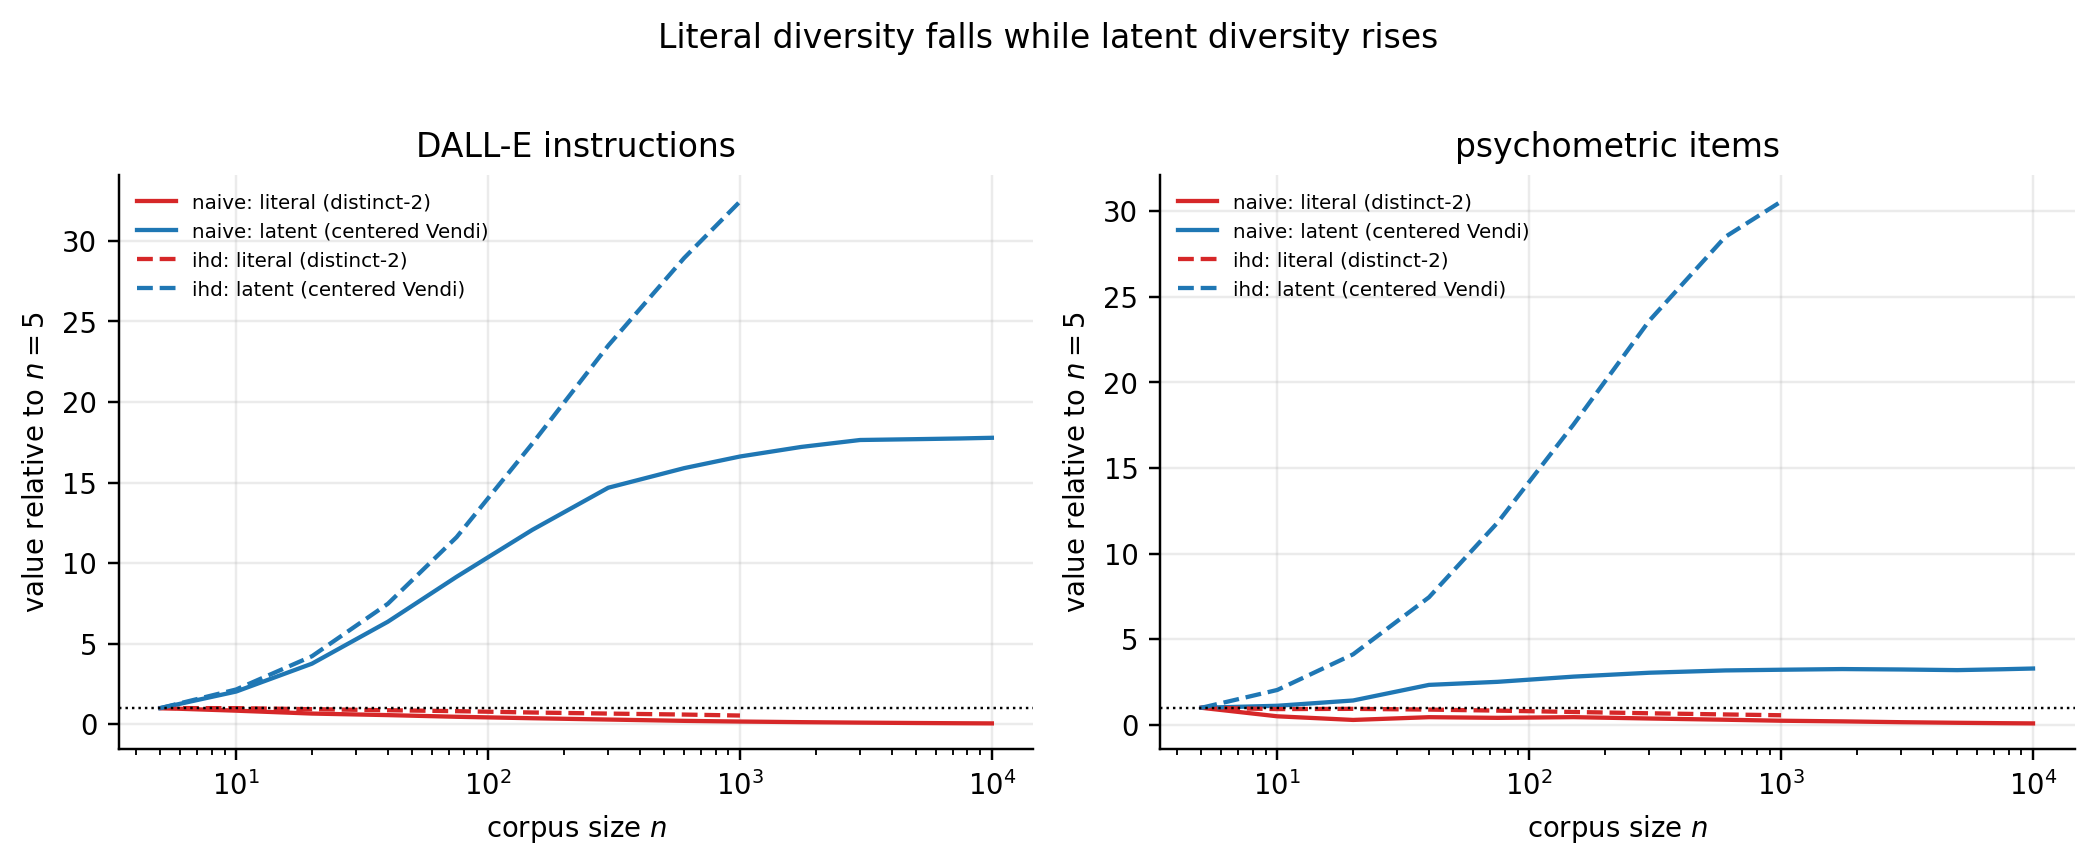
\includegraphics[keepaspectratio,alt={Figure 5. The decoupling, normalized to each series\textquotesingle{} value at n = 5. Literal diversity falls monotonically while latent diversity rises: two measurements of two different quantities that one word, "diversity", has been covering for.}]{figures/fig11_literal_vs_latent.png}}

\emph{Figure 5. The decoupling, normalized to each
series\textquotesingle{} value at n = 5. Literal diversity falls
monotonically while latent diversity rises: two measurements of two
different quantities that one word, "diversity", has been covering for.}

\subsubsection{\texorpdfstring{7.2 Competitive comparison at matched
\emph{n}}{7.2 Competitive comparison at matched n}}\label{72-competitive-comparison-at-matched-n}

All seven arms, real corpora, DALL·E domain, every arm evaluated on the
same number of accepted items (\emph{n} = 200):

{\footnotesize
\begin{longtable}[]{@{}>{\raggedright\arraybackslash}p{\dimexpr 0.2827\linewidth-2\tabcolsep\relax}>{\raggedright\arraybackslash}p{\dimexpr 0.1283\linewidth-2\tabcolsep\relax}>{\raggedright\arraybackslash}p{\dimexpr 0.1414\linewidth-2\tabcolsep\relax}>{\raggedright\arraybackslash}p{\dimexpr 0.1571\linewidth-2\tabcolsep\relax}>{\raggedright\arraybackslash}p{\dimexpr 0.1371\linewidth-2\tabcolsep\relax}>{\raggedright\arraybackslash}p{\dimexpr 0.1533\linewidth-2\tabcolsep\relax}@{}}
\toprule\noalign{}
arm & distinct-2 ↑ & self-repetition ↓ & \emph{n}-gram Vendi ↑ &
centered Vendi ↑ & median NN distance ↑ \\
\midrule\noalign{}
\endhead
\bottomrule\noalign{}
\endlastfoot
naive & 0.293 & 0.345 & 107.6 & 50.45 & 0.045 \\
high temperature & 0.291 & 0.339 & 109.0 & 49.44 & 0.045 \\
Evol-Instruct & 0.386 & 0.353 & 108.1 & 50.10 & \textbf{0.021} \\
Self-Instruct & 0.545 & 0.131 & 140.4 & 67.45 & 0.121 \\
persona conditioning & 0.582 & 0.130 & 124.7 & 56.50 & 0.080 \\
\textbf{RAC} & 0.660 & 0.068 & 167.0 & 77.67 & 0.171 \\
\textbf{RAC + vision steering} & \textbf{0.699} & \textbf{0.040} &
\textbf{170.9} & \textbf{91.97} & \textbf{0.192} \\
\end{longtable}}

RAC wins every column, and adding vision steering improves on the
text-only variant by a further 18\% in centered Vendi. Three baselines
fail in different ways, and the failures are informative. High
temperature buys nothing: distinct-2 of 0.291 against
naive\textquotesingle s 0.293, an identical median nearest-neighbour
distance of 0.045. Evol-Instruct comes out \emph{worse than naive} at
the one thing a diversity method exists for --- its median
nearest-neighbour distance is 0.021 against naive\textquotesingle s
0.045, so it produces items closer to the existing corpus than
independent sampling does. The mechanism is working as designed:
mutating an existing item produces a neighbour of that item. It raises
distinct-2 (0.386 against 0.293) because the mutations reword things, so
a purely literal evaluation would score it as an improvement; measuring
both levels is what catches it. Self-Instruct\textquotesingle s guard is
literal and defends the literal level only: it achieves the best
self-repetition of any baseline (0.131 --- its ROUGE filter is doing
real work) while its centered Vendi trails RAC by ten points. A ROUGE-L
threshold cannot see semantic redundancy, and semantic redundancy is
what remains once the lexical kind is filtered.

\pandocbounded{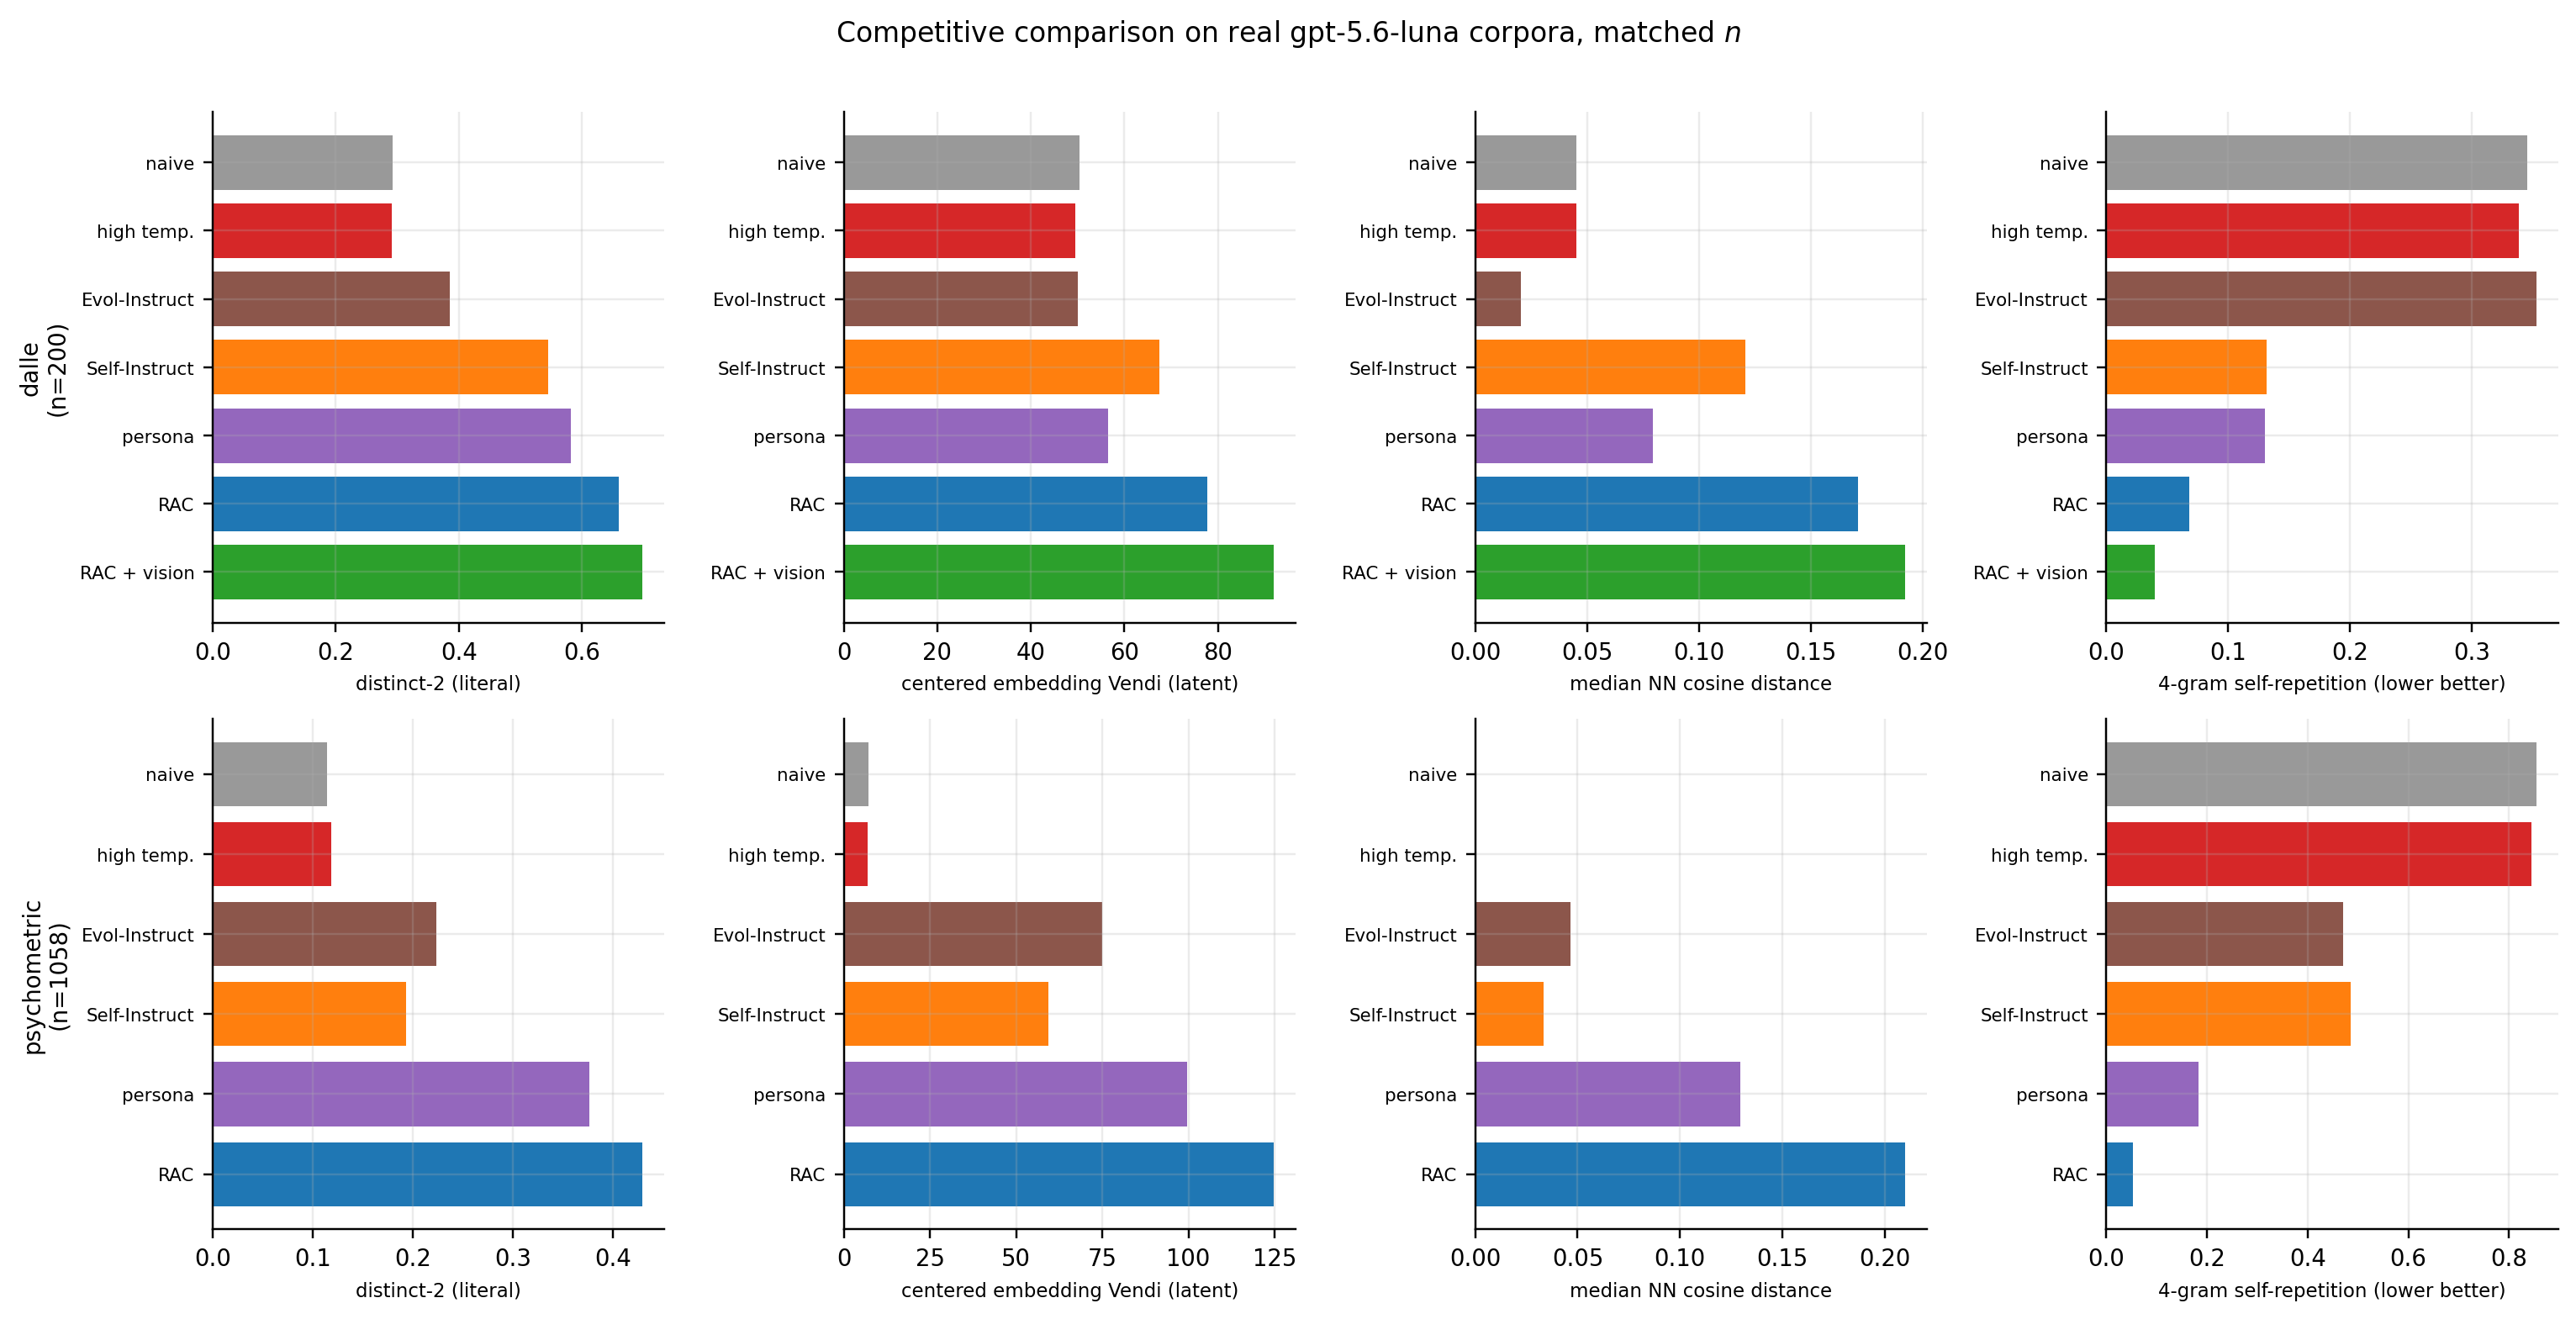
\includegraphics[keepaspectratio,alt={Figure 6. Competitive comparison on real corpora at matched n, both text domains, across four metrics.}]{figures/fig14_arms.png}}

\emph{Figure 6. Competitive comparison on real corpora at matched n,
both text domains, across four metrics.}

The psychometric domain repeats the ordering on all six arms at matched
\emph{n} = 1,999:

{\footnotesize
\begin{longtable}[]{@{}>{\raggedright\arraybackslash}p{\dimexpr 0.2542\linewidth-2\tabcolsep\relax}>{\raggedright\arraybackslash}p{\dimexpr 0.1154\linewidth-2\tabcolsep\relax}>{\raggedright\arraybackslash}p{\dimexpr 0.1154\linewidth-2\tabcolsep\relax}>{\raggedright\arraybackslash}p{\dimexpr 0.1271\linewidth-2\tabcolsep\relax}>{\raggedright\arraybackslash}p{\dimexpr 0.1413\linewidth-2\tabcolsep\relax}>{\raggedright\arraybackslash}p{\dimexpr 0.1233\linewidth-2\tabcolsep\relax}>{\raggedright\arraybackslash}p{\dimexpr 0.1233\linewidth-2\tabcolsep\relax}@{}}
\toprule\noalign{}
arm & exact-dup ↓ & distinct-2 ↑ & self-repetition ↓ & \emph{n}-gram
Vendi ↑ & centered Vendi ↑ & median NN dist ↑ \\
\midrule\noalign{}
\endhead
\bottomrule\noalign{}
\endlastfoot
naive & 0.668 & 0.114 & 0.855 & 11.8 & 7.1 & 0.000 \\
high temperature & 0.660 & 0.119 & 0.845 & 12.2 & 7.0 & 0.000 \\
Self-Instruct & 0.026 & 0.193 & 0.485 & 288.8 & 59.3 & 0.033 \\
Evol-Instruct & 0.025 & 0.224 & 0.470 & 307.4 & 75.0 & 0.047 \\
persona conditioning & 0.004 & 0.377 & 0.184 & 545.6 & 99.7 & 0.130 \\
\textbf{RAC} & \textbf{0.000} & \textbf{0.429} & \textbf{0.053} &
\textbf{644.3} & \textbf{124.8} & \textbf{0.210} \\
\end{longtable}}

RAC wins every column here as well, beating the strongest baseline by
25\% in centered Vendi and by a factor of 3.5 in self-repetition. The
two undiversified arms score an order of magnitude worse on the latent
measures because their duplicate rates of 0.66--0.67 mean the embedding
metric is largely measuring repetition; deduplicating first raises them
to 19.8 and 20.7, still far behind every conditioned method, and their
median nearest-neighbour distance is exactly zero --- the median item
has a perfect twin.

\subsubsection{7.3 Head-to-head against released instruction
corpora}\label{73-head-to-head-against-released-instruction-corpora}

Reimplementations are the right experiment for isolating mechanisms and
the wrong one for the question \emph{is this actually good?} So we also
compare against the released artifacts of the three most-used
synthetic-instruction methods --- Alpaca (52k), PersonaHub (50k) and
WizardLM Evol-Instruct (143k).

\textbf{Protocol.} The human-written reference is databricks-dolly-15k,
split into two disjoint 3,000-item halves: a STEER half our method may
read as embeddings on the selection side, and an evaluation half that
nothing in any pipeline ever reads and at which no corpus, ours or
released, was ever aimed. All scores are on the evaluation half.
Estimator: Naeem et al. (2020) coverage/density with reference-side
\emph{k}-NN radii, reported as AUC over \emph{k} ∈ \{3, 5, 10, 20\}; the
radii are a property of the reference alone, identical for every corpus,
with nothing tunable per corpus. Every corpus is evaluated as a uniform
random sample at matched \emph{n} = 450. Our arms and the reimplemented
baselines all receive the same 175 human seed tasks --- the seed set
Alpaca was built from --- the same generator, and the same budget of
2,400 generator calls, with rejection and selection losses counted
rather than hidden. The generator never sees a reference word in any
arm.

\pandocbounded{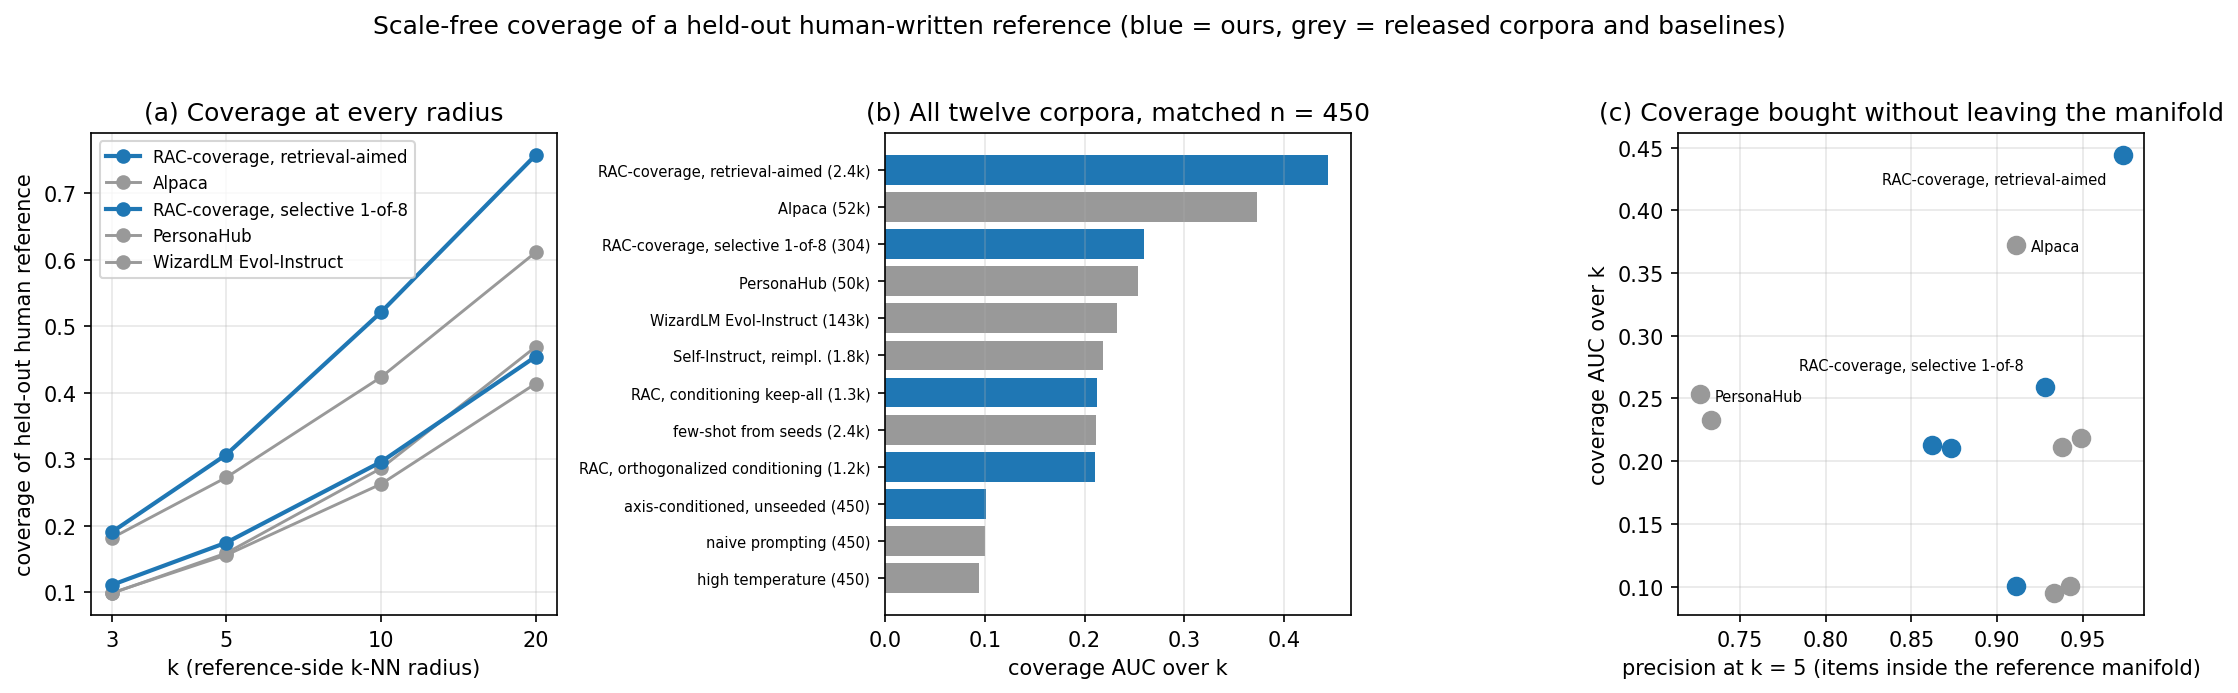
\includegraphics[keepaspectratio,alt={Figure 7. Scale-free coverage of a held-out human-written reference. (a) Coverage at every reference-side radius. (b) All twelve corpora at matched evaluated n = 450. (c) Coverage against precision: the winning corpus is also the one that stays inside the reference manifold.}]{figures/fig_h2h_scalefree.png}}

\emph{Figure 7. Scale-free coverage of a held-out human-written
reference. (a) Coverage at every reference-side radius. (b) All twelve
corpora at matched evaluated n = 450. (c) Coverage against precision:
the winning corpus is also the one that stays inside the reference
manifold.}

{\footnotesize
\begin{longtable}[]{@{}>{\raggedright\arraybackslash}p{\dimexpr 0.3505\linewidth-2\tabcolsep\relax}>{\raggedright\arraybackslash}p{\dimexpr 0.3159\linewidth-2\tabcolsep\relax}>{\raggedright\arraybackslash}p{\dimexpr 0.1697\linewidth-2\tabcolsep\relax}>{\raggedright\arraybackslash}p{\dimexpr 0.1639\linewidth-2\tabcolsep\relax}@{}}
\toprule\noalign{}
rank & corpus & AUC & precision \\
\midrule\noalign{}
\endhead
\bottomrule\noalign{}
\endlastfoot
1 & \textbf{RAC-coverage, retrieval-aimed (2.4k)} & \textbf{0.4441} &
\textbf{0.973} \\
2 & Alpaca (Self-Instruct, 52k) & 0.3722 & 0.87 \\
3 & RAC-coverage, selective 1-of-8 (304) & 0.2591 & 0.93 \\
4 & PersonaHub (50k) & 0.2532 & 0.78 \\
5 & WizardLM Evol-Instruct (143k) & 0.2329 & 0.77 \\
6 & Self-Instruct (reimpl., same seeds/budget) & 0.2188 & \\
7 & RAC, conditioning keep-all & 0.2127 & \\
8 & few-shot from seeds & 0.2114 & \\
9 & RAC, orthogonalized conditioning & 0.2102 & \\
10--12 & axis-conditioned unseeded / naive / high temperature &
0.0947--0.1008 & \\
\end{longtable}}

First place, 19\% above Alpaca, with the highest precision in the field,
at roughly one-twentieth of Alpaca\textquotesingle s generation budget.
An interim measurement at 22\% of budget (\emph{n} = 528) already scored
0.4276 against Alpaca\textquotesingle s 0.3666 on the same protocol, so
the result does not depend on final corpus size. PersonaHub and WizardLM
finish below our 304-item selective arm despite 20--60× the scale.

\textbf{What the ranking is a claim about.} Our retrieval-aimed arm
reads a sample of the target distribution, as embeddings, on the
steering side; none of the released corpora had such an input, so first
place is not a like-for-like result. The like-for-like comparison is
rows 6--9, where our configurations that never touch the STEER half sit
at parity with the Self-Instruct family. The precise claim is therefore:
\textbf{given a specification of the space to cover --- even one the
generator never reads a word of --- retrieval-aimed, density-adaptive
conditioning covers it substantially better than the strongest seeded
baseline covers it at twenty times the budget.} That is a capability
statement about targeted generation, and it is the one the ablation
supports.

Budget-matched ablation, 2,400 generator calls each, same evaluation
half. These rows are \textbf{not} at matched \emph{n}: \texttt{kept} is
each arm\textquotesingle s own surviving corpus size after rejection and
selection losses, and the coverage estimator is monotone in items, so an
arm with fewer kept items is penalized for that alone.

{\footnotesize
\begin{longtable}[]{@{}>{\raggedright\arraybackslash}p{\dimexpr 0.3823\linewidth-2\tabcolsep\relax}>{\raggedright\arraybackslash}p{\dimexpr 0.0851\linewidth-2\tabcolsep\relax}>{\raggedright\arraybackslash}p{\dimexpr 0.1473\linewidth-2\tabcolsep\relax}>{\raggedright\arraybackslash}p{\dimexpr 0.1006\linewidth-2\tabcolsep\relax}>{\raggedright\arraybackslash}p{\dimexpr 0.1423\linewidth-2\tabcolsep\relax}>{\raggedright\arraybackslash}p{\dimexpr 0.1423\linewidth-2\tabcolsep\relax}@{}}
\toprule\noalign{}
configuration & kept & AUC & density & precision & recall \\
\midrule\noalign{}
\endhead
\bottomrule\noalign{}
\endlastfoot
\textbf{RAC-coverage, retrieval-aimed} & 2,398 & \textbf{0.6597} & 1.637
& \textbf{0.960} & \textbf{0.178} \\
Self-Instruct (reimpl.) & 1,833 & 0.3262 & 1.050 & 0.949 & 0.161 \\
few-shot from seeds & 2,399 & 0.3246 & 1.052 & 0.935 & 0.152 \\
conditioning, keep-all & 1,310 & 0.3147 & 0.704 & 0.864 & 0.068 \\
orthogonalized conditioning & 1,152 & 0.2941 & 0.718 & 0.873 & 0.101 \\
selective (1-of-8) & 304 & 0.2591 & 1.009 & 0.928 & 0.099 \\
\end{longtable}}

The ablation attributes the margin. Retrieval-aiming and the
radius-adaptive mode carry it (row 1 against rows 2--4); few-shot
anchoring to the human seeds accounts for most of the
baselines\textquotesingle{} scores (row 3 against the unseeded arms at
0.09--0.10); Self-Instruct\textquotesingle s ROUGE filter adds 0.0016
over bare few-shot; and both selection (row 6) and orthogonalized
conditioning (row 5) \emph{reduce} coverage relative to keeping
everything, which is §3 arriving in the ablation table --- coverage is
monotone and measure-seeking, so discarding and occupied-span avoidance
are each counter-productive under this objective where both are
load-bearing under max-min.

Two arms keep every candidate that clears the gate and therefore carry
the generator\textquotesingle s repeats: at full corpus size the
retrieval-aimed arm is 21.1\% exact duplicates and the
few-shot-from-seeds baseline 20.6\%, while every arm that selects at all
sits at exactly 0.000. Since a repeated instruction covers a ball that
is already covered, those repeats spend evaluated slots for nothing.
Re-scoring every corpus after collapsing it to its distinct
instructions, at the same radii and the same evaluated \emph{n}, raises
the retrieval-aimed arm from 0.4532 to 0.4752 and widens its margin over
Alpaca from 16\% to 21\%. \textbf{The duplicates were costing coverage
rather than manufacturing it, and the headline number is the
conservative one.} Only the two keep-everything arms move; the ordering
is otherwise unchanged.

\subsubsection{7.4 The exam bank: a measured enemy-item
radius}\label{74-the-exam-bank-a-measured-enemy-item-radius}

Exam items invert the semantics of the other domains. Two operational
items closer than δ are \emph{enemy items} --- seeing one gives away the
other --- which is a test-security failure at any bank size, so the
floor is a hard constraint rather than a term in a weighted sum, and the
min-distance check must be exact against the full bank rather than
subsampled. Item templates expose few manipulable slots, so each mode is
a low-dimensional disk and the δ-packing number of a bank is finite and
small: a bank has a \emph{capacity}, and the operative question is what
fraction of a nominal bank is actually usable.

That turns on δ, so we measured it rather than assuming it. 236 item
pairs drawn from a human-written bank across the full range of embedding
distance were put to a blind psychometric adjudication --- does seeing
one item give a material advantage on the other, through a shared fact,
a re-skin, or matched distractor misconceptions --- with the judge shown
neither the distance nor the provenance. A logistic fit of enemy
verdicts on distance crosses 50\% at \textbf{δ = 0.0409}. The crossing
is weakly identified at this sample size --- a nonparametric bootstrap
over the same adjudications gives a median of 0.0419 with 95\% CI
{[}−0.0078, 0.0780{]} on 24 positives --- so δ should be read as an
order of magnitude rather than a constant. What \emph{is} well
determined is the ranking: embedding distance separates adjudicated
enemy pairs from safe ones at AUC 0.9208.

Applying that radius to real banks --- six generation policies at 2,500
items each, and the human bank under identical treatment:

{\footnotesize
\begin{longtable}[]{@{}>{\raggedright\arraybackslash}p{\dimexpr 0.4121\linewidth-2\tabcolsep\relax}>{\raggedright\arraybackslash}p{\dimexpr 0.1692\linewidth-2\tabcolsep\relax}>{\raggedright\arraybackslash}p{\dimexpr 0.1971\linewidth-2\tabcolsep\relax}>{\raggedright\arraybackslash}p{\dimexpr 0.2216\linewidth-2\tabcolsep\relax}@{}}
\toprule\noalign{}
bank & exact-dup & items with an enemy & usable after the floor \\
\midrule\noalign{}
\endhead
\bottomrule\noalign{}
\endlastfoot
MMLU (human-written) & 0.024 & 0.092 & 2,373 (94.9\%) \\
naive prompting & 0.695 & 0.884 & 382 (15.3\%) \\
high temperature & 0.710 & 0.897 & 365 (14.6\%) \\
Self-Instruct & 0.047 & 0.616 & 1,373 (54.9\%) \\
Evol-Instruct & 0.012 & 0.424 & 1,870 (74.8\%) \\
persona conditioning & 0.007 & 0.047 & 2,425 (97.0\%) \\
\textbf{RAC} & \textbf{0.000} & \textbf{0.000} & \textbf{1,999
(100.0\%)} \\
\end{longtable}}

A naively generated bank of 2,500 items yields 382 that can coexist on
one form --- 15\% of nominal capacity, against 94.9\% for the human bank
--- and temperature makes it slightly worse. Both conditioned policies
exceed the human bank\textquotesingle s usable fraction, and the
axis-conditioned bank contains \textbf{no enemy pair at all} at the
judged radius, a result that holds across the full 1,999-item bank at
every δ up to 0.0776 under three of four embedders. Two qualifications
belong with that number: it is measured at 1,999 items against the naive
bank\textquotesingle s 2,500, and about 80\% of the naive
bank\textquotesingle s lost capacity is exact duplication, which needs
no radius to detect.

\textbf{Against the human bank itself.} MMLU is \textasciitilde14,000
multiple-choice items from real practice exams and textbooks across 57
subjects, by many authors, with editorial review, over years. At matched
\emph{n} = 1,000 with identical metric code:

{\footnotesize
\begin{longtable}[]{@{}>{\raggedright\arraybackslash}p{\dimexpr 0.2817\linewidth-2\tabcolsep\relax}>{\raggedright\arraybackslash}p{\dimexpr 0.1138\linewidth-2\tabcolsep\relax}>{\raggedright\arraybackslash}p{\dimexpr 0.1138\linewidth-2\tabcolsep\relax}>{\raggedright\arraybackslash}p{\dimexpr 0.1211\linewidth-2\tabcolsep\relax}>{\raggedright\arraybackslash}p{\dimexpr 0.1346\linewidth-2\tabcolsep\relax}>{\raggedright\arraybackslash}p{\dimexpr 0.1175\linewidth-2\tabcolsep\relax}>{\raggedright\arraybackslash}p{\dimexpr 0.1175\linewidth-2\tabcolsep\relax}@{}}
\toprule\noalign{}
source & exact-dup ↓ & distinct-2 ↑ & self-repetition ↓ & \emph{n}-gram
Vendi ↑ & centered Vendi ↑ & median NN dist ↑ \\
\midrule\noalign{}
\endhead
\bottomrule\noalign{}
\endlastfoot
\textbf{MMLU (human-written)} & 0.0040 & \textbf{0.5888} & 0.0585 &
495.2 & \textbf{197.50} & \textbf{0.2838} \\
persona conditioning & 0.0040 & 0.3887 & 0.1711 & 543.3 & 99.71 &
0.1346 \\
\textbf{RAC} & \textbf{0.0000} & 0.4377 & \textbf{0.0503} &
\textbf{622.2} & 135.58 & 0.2235 \\
\end{longtable}}

We \emph{beat} MMLU on exact duplication (the human bank has some), on
4-gram self-repetition, and on \emph{n}-gram Vendi: \textbf{our items
reuse less language than human-written ones do.} We \emph{lose} on the
semantic measures --- centered Vendi 135.6 against 197.5 and median
nearest-neighbour distance 0.224 against 0.284 --- reaching roughly 69\%
of a human exam bank\textquotesingle s effective semantic diversity.
That gap is the measure of what is left, and it is the
reachable-dimension question of §4 rather than a tuning problem:
MMLU\textquotesingle s spread comes from 57 genuinely different
subjects, ours from an axis lattice a single model proposed in one call
and refined a handful of times.

\subsubsection{7.5 Separation on channels the method never
optimizes}\label{75-separation-on-channels-the-method-never-optimizes}

Every comparison so far is scored either in the embedding the loop
selects on or in a surface statistic correlated with it. The strongest
evidence available is a channel that is \emph{causally downstream of the
artifact and upstream of nothing the loop reads}. Each artifact domain
has one, and RAC separates on all three at matched generator budget
(Figure 1).

\textbf{Poems: prosody.} Nothing in the loop measures metre, rhyme or
line construction, and \texttt{nomic-embed-text} is a semantic model
nearly blind to them. We score twenty-two prosodic and structural
features --- line and stanza counts, syllables per line and their
regularity, rhyme density, alliteration, punctuation and clause rates,
type--token ratio, person and tense markers --- at a \textbf{matched
generator budget of 328 calls each}. The naive arm spends its 328 calls
on 328 poems where RAC spends them on 60, so we compare equal-sized
corpora by drawing 60 of the naive arm\textquotesingle s 328 at random,
which is generous to the baseline: 60 drawn from 328 distinct items
spread further than any 60 consecutive ones.

{\footnotesize
\begin{longtable}[]{@{}>{\raggedright\arraybackslash}p{\dimexpr 0.5520\linewidth-2\tabcolsep\relax}>{\raggedright\arraybackslash}p{\dimexpr 0.2279\linewidth-2\tabcolsep\relax}>{\raggedright\arraybackslash}p{\dimexpr 0.2202\linewidth-2\tabcolsep\relax}@{}}
\toprule\noalign{}
& prosodic spread & median NN \\
\midrule\noalign{}
\endhead
\bottomrule\noalign{}
\endlastfoot
RAC (60 poems, 328 calls) & \textbf{10.23} & \textbf{5.73} \\
naive, full (328 poems, 328 calls) & 4.56 & 2.22 \\
naive, 60-subsample (mean of 200 draws) & 4.54 & 2.63 \\
\textbf{ratio, RAC / naive-subsample} & \textbf{2.25×} &
\textbf{2.18×} \\
\end{longtable}}

RAC exceeds the naive arm on \textbf{200 of 200 random draws} on both
statistics. Removing the eight length-scale features --- the hard case,
since RAC poems are longer on average and length inflates several of the
twenty-two --- leaves spread at 2.02× and median nearest-neighbour
distance at 1.84×, still 200 of 200.

\textbf{Exam items: architecture.} Item writers attend to how the work
divides between stem and options, whether options are parallel in form
and balanced in length, whether the stem is negated, how many options
there are, and whether flaw markers like absolute terms or "all of the
above" appear. Scored on thirteen such features --- ratios and rates, so
a longer item does not automatically read as a different one --- and
\textbf{with every exact duplicate removed from both corpora first}, so
the comparison cannot restate the duplication of §7.1:

{\footnotesize
\begin{longtable}[]{@{}>{\raggedright\arraybackslash}p{\dimexpr 0.3329\linewidth-2\tabcolsep\relax}>{\raggedright\arraybackslash}p{\dimexpr 0.1438\linewidth-2\tabcolsep\relax}>{\raggedright\arraybackslash}p{\dimexpr 0.1844\linewidth-2\tabcolsep\relax}>{\raggedright\arraybackslash}p{\dimexpr 0.1803\linewidth-2\tabcolsep\relax}>{\raggedright\arraybackslash}p{\dimexpr 0.1585\linewidth-2\tabcolsep\relax}@{}}
\toprule\noalign{}
& distinct items & distinct architectures & items per architecture &
structural spread \\
\midrule\noalign{}
\endhead
\bottomrule\noalign{}
\endlastfoot
\textbf{RAC} & 1,999 & \textbf{1,951 (97.6\%)} & \textbf{1.0} &
\textbf{5.06} \\
naive & 2,645 & 1,160 (43.9\%) & 2.3 & 3.14 \\
\end{longtable}}

RAC produces very nearly one architecture per item. The naive bank
reuses each of its 1,160 architectures 2.3 times over, and \textbf{its
median deduplicated item still has an exact structural twin at distance
zero} --- items that differ in wording while being built identically,
which no exact-match deduplication and no embedding metric in this paper
detects. Structural spread is 1.61× at matched \emph{n}, on 50 of 50
random draws. Option count is the sharpest single case: it never varies
at all in the naive bank.

\textbf{Images: pixel statistics.} Nine statistics computed from the
render itself --- luminance, contrast, tonal range, saturation,
colourfulness, hue entropy, edge density, edge anisotropy, and where the
visual weight sits --- with every corpus sampled to a matched \emph{n} =
60 and scored from its highest available render tier. On mean pairwise
distance in the globally standardized feature space, \textbf{every one
of our eleven corpora exceeds every one of the five published
baselines}, with no overlap at the boundary (3.66 against 3.24): a
Mann--Whitney \emph{U} of 55, the maximum attainable for these group
sizes, at \emph{p} = 0.0002, and a group-mean ratio of \textbf{1.53×},
bootstrap 95\% CI {[}1.38, 1.68{]}. Dropping any single feature and
recomputing leaves the ratio between 1.50× and 1.59×, so it is not
carried by one statistic. On median nearest-neighbour distance in the
same space --- which answers whether the corpora are less \emph{locally
crowded}, and which outliers cannot inflate --- our arms run 1.30 to
1.95 against the baselines\textquotesingle{} 1.15 to 1.38, 54 of 55
comparisons in our favour (\emph{U} = 54, \emph{p} = 0.0005, 1.37×
{[}1.25, 1.48{]} on the means). The two statistics fail in different
directions and agree here.

The measurement rests on one choice with an obvious alternative that
gives a misleading answer. \textbf{Use a distance statistic, not a
spectral one, on a designed feature channel.} Vendi, which we use
throughout for embeddings, is the exponentiated entropy of a covariance
spectrum: it scores the effective \emph{dimensionality} of variation
rather than its extent. On a 768-dimensional embedding no single
direction can dominate the spectrum and the distinction rarely bites. On
a nine-dimensional feature vector it dominates completely, and a corpus
that spreads far along two or three optical directions scores
\emph{below} one that wobbles slightly along all nine --- the spectral
estimator answers "how many optical directions vary", which is not the
question. On mean pairwise distance, optical spread correlates with CLIP
diversity at \emph{r} = +0.76 (\emph{p} = 0.003) across the thirteen
corpora; under the spectral estimator the same corpora correlate at
−0.60. Degradation is also worth ruling out, since blurred renders move
pixel statistics a long way for no gain in genuine variety, and it does
not explain the gap: blurring \emph{k} of sixty baseline renders lowers
CLIP Vendi monotonically, 43.81 to 41.72 as \emph{k} runs 0 to 30, so an
embedding-space objective is penalized rather than rewarded for
admitting degraded images, and mean corpus sharpness is uncorrelated
with CLIP Vendi across the thirteen corpora (+0.19, \emph{p} = 0.53).

Together these three comparisons say the same thing in three modalities.
\textbf{The steering produces artifacts that differ from one another in
dimensions no part of the pipeline scores}, which is not something a
selection rule can manufacture for itself. §8 asks how much of that is
attributable to any individual axis, and the answer is more complicated.
\textbf{Two further comparisons on these channels belong to the
companion paper on proxy embeddings}, and are stated there in full. The
first runs the other way: on non-semantic structural signatures --- a
16×16 luminance layout map, a tiling score, a hue histogram --- the
published baselines are \emph{better} than our arms, so our corpora
occupy a wider region of pixel space while repeating their compositional
scaffolding more often within it; literal-space structural bans halve
the palette twins and do not close the gap (companion §4.6). The second
is reassurance about the instrument: six exam-item corpora scored under
four independent representations --- CLIP text, TF-IDF, the prosodic
vector and a function-word profile, three of which the method never
optimizes --- rank the same way at a mean Kendall τ of +0.83 across
their six pairings, and RAC ranks first under every one of them
(companion §4.4).

\subsubsection{7.6 What the coverage score buys
downstream}\label{76-what-the-coverage-score-buys-downstream}

A coverage number earns its place only if something a practitioner wants
depends on it. Extending the retrieval-aimed policy to 24,000 generator
calls:

{\footnotesize
\begin{longtable}[]{@{}>{\raggedright\arraybackslash}p{\dimexpr 0.3504\linewidth-2\tabcolsep\relax}>{\raggedright\arraybackslash}p{\dimexpr 0.1670\linewidth-2\tabcolsep\relax}>{\raggedright\arraybackslash}p{\dimexpr 0.0431\linewidth-2\tabcolsep\relax}>{\raggedright\arraybackslash}p{\dimexpr 0.1294\linewidth-2\tabcolsep\relax}>{\raggedright\arraybackslash}p{\dimexpr 0.1670\linewidth-2\tabcolsep\relax}>{\raggedright\arraybackslash}p{\dimexpr 0.1430\linewidth-2\tabcolsep\relax}@{}}
\toprule\noalign{}
RAC items & coverage AUC & & RAC items & coverage AUC & Δ per 1,000 \\
\midrule\noalign{}
\endhead
\bottomrule\noalign{}
\endlastfoot
100 & 0.1878 & & 1,000 & 0.5394 & --- \\
250 & 0.3023 & & 2,000 & 0.6323 & +0.093 \\
\textbf{400} & \textbf{0.3938} & & 5,000 & 0.7552 & +0.026 \\
500 & 0.4286 & & 10,000 & 0.8107 & +0.008 \\
750 & 0.5014 & & 23,993 & \textbf{0.8501} & +0.002 \\
\end{longtable}}

The 0.3722 reported for Alpaca is a uniform random 450-item sample of
its 52,002 items, not a score for the whole corpus; the estimator is
monotone in items and this paper does not measure Alpaca at its own
size. The comparison available is therefore a near-matched one:
\textbf{four hundred items of this corpus score 0.3938, above that
450-item Alpaca sample and at a slightly smaller \emph{n}}. Dividing a
matched-\emph{n} score by a full-corpus item count is not a supportable
operation and no such ratio is reported. The completed 24,000-call run
reaches 0.8501 at its own size of 23,993 items for \$4.64 and 130
minutes --- a figure at that \emph{n}, not comparable with any
matched-\emph{n} score. Per thousand generator calls at the matched
budget this policy converts calls into coverage at 0.275 against 0.136
for Self-Instruct and 0.135 for few-shot: \textbf{twice as efficiently
as the strongest seeded baseline}.

\textbf{The ceiling is visible in the same run, from outside.} This
policy discards nothing, so every repetition the generator emits is
recorded and the duplicate rate reads out how much it has left to say:
0.233 at 2,400 calls, 0.394 at 10,000, 0.544 at 23,993. The 0.8501
corpus rests on 10,935 distinct instructions bought with 13,058 wasted
calls, and marginal coverage per thousand items collapses fortyfold
across the run. This is the conditional-dimension result of §4 measured
on the generation process rather than inferred from a coverage curve.

\textbf{Which mode spends the budget, and which earns the coverage.} The
radius-adaptive rule splits the run unevenly --- 19,967 items (83.2\%)
in imitate mode against 4,026 (16.8\%) under axis conditioning --- and
since coverage is computed on the union, the headline number alone
cannot say which mode produced it. Decomposing it says something better
than the headline does.

{\footnotesize
\begin{longtable}[]{@{}>{\raggedright\arraybackslash}p{\dimexpr 0.3995\linewidth-2\tabcolsep\relax}>{\raggedright\arraybackslash}p{\dimexpr 0.1169\linewidth-2\tabcolsep\relax}>{\raggedright\arraybackslash}p{\dimexpr 0.2135\linewidth-2\tabcolsep\relax}>{\raggedright\arraybackslash}p{\dimexpr 0.2701\linewidth-2\tabcolsep\relax}@{}}
\toprule\noalign{}
& items & exact-duplicate rate & share in top-4 six-word openings \\
\midrule\noalign{}
\endhead
\bottomrule\noalign{}
\endlastfoot
imitate & 19,967 & \textbf{0.654} & 31.6\% \\
axis-conditioned & 4,026 & \textbf{0.000} & 1.4\% \\
\end{longtable}}

\textbf{Axis conditioning produced no exact duplicate in four thousand
items}; the corpus-level 0.544 is imitation\textquotesingle s, not the
method\textquotesingle s. Scoring the two modes at matched item counts,
so the comparison is not "more items cover more" --- five draws per
cell, 4,000-item reference --- imitation leads at 500 items (0.235
against 0.211 at \emph{k} = 5), the two are indistinguishable at 1,000,
and axis conditioning leads from 2,000 on (0.529 against 0.500 at
\emph{n} = 4,000). The crossover is what the design predicts: imitation
reaches the dense core quickly because that is where reference points
are numerous, then saturates as it begins repeating, while conditioning
keeps reaching new regions. The two are also complementary rather than
redundant: at \emph{n} = 4,000 and \emph{k} = 5, imitation alone reaches
14.9\% of the reference that conditioning misses, conditioning alone
reaches 18.0\% that imitation misses, 34.9\% is reached by both and
32.1\% by neither. Neither mode approaches the union on its own, and
\textbf{conditioning contributes the larger unique share on a sixth of
the budget}.

\textbf{The wasted budget is a prompting failure, and fixing it is a
one-line change.} The imitate branch shows the generator three
neighbours of the target and asks for another item of the same kind; it
is not shown what it has already written there, so a dense target hit
repeatedly receives the same three examples every time and returns the
same item. The conditioning branch has always passed its own nearby
outputs as explicit negatives; the imitate branch computed them and
discarded them. Two 1,200-call arms with identical seeds and targets,
differing only in that:

{\footnotesize
\begin{longtable}[]{@{}>{\raggedright\arraybackslash}p{\dimexpr 0.5679\linewidth-2\tabcolsep\relax}>{\raggedright\arraybackslash}p{\dimexpr 0.2040\linewidth-2\tabcolsep\relax}>{\raggedright\arraybackslash}p{\dimexpr 0.2281\linewidth-2\tabcolsep\relax}@{}}
\toprule\noalign{}
& as published & + negatives \\
\midrule\noalign{}
\endhead
\bottomrule\noalign{}
\endlastfoot
duplicate rate, imitate branch & 0.145 & \textbf{0.025} \\
duplicate rate, conditioning branch & 0.000 & 0.000 \\
share of the branch in its four commonest openings & 32.5\% &
\textbf{9.0\%} \\
distinct items per generator call & 0.897 & \textbf{0.982} \\
coverage AUC & 0.5326 & \textbf{0.5492} \\
\end{longtable}}

The duplicate rate falls by 83\%, template mass by a factor of three and
a half, and --- the quantity a budget actually buys --- distinct items
per call rise from 0.897 to 0.982, with coverage improving rather than
paying for it, because the calls recovered from repetition are spent on
targets not yet reached. A neighbourhood whose task family has a small
extension cannot be rescued this way --- there are finitely many musical
instruments --- and the obvious next move, handing such a neighbourhood
to the conditioning branch, makes matters worse: duplicate rate 0.041
against 0.025, distinct per call 0.970 against 0.982, coverage AUC
0.5355 against 0.5492. The radius-adaptive rationale explains why. A
dense target\textquotesingle s ball is small, so a diversified item
lands outside it and covers nothing while a merely repetitive one at
least covers its own neighbourhood; in a dense core typicality is what
coverage wants, and the repetition is corrected by telling the generator
what it already wrote rather than by abandoning imitation.

\textbf{Seven times as many queries have a usable neighbour.} Taking
each held-out instruction\textquotesingle s nearest neighbour in a
950-item pool from each corpus, the retrieval-aimed corpus serves 17.6\%
of queries at similarity ≥ 0.70 against 11.8\% for Alpaca, 3.8\% for
Persona-Hub, 3.6\% for WizardLM and 2.4\% for plain conditioning:
\textbf{7.3× as many as plain conditioning and 4.6× as many as the best
published baseline, at identical pool size.} Coverage AUC predicts this
at \emph{r} = 0.972. That correlation is close to a self-correlation and
should be read as collinearity rather than corroboration --- coverage
AUC counts reference points with a generated item inside their
\emph{k}-NN ball, and \emph{queries served at 0.70} counts held-out
queries with a generated item inside a fixed-similarity ball, the same
functional under two radius rules. The table\textquotesingle s content
is the ordering of the pools and the size of the gaps.

\textbf{And the covering pool wins at every retrieval depth.} Prompting
a Qwen2.5-0.5B base model with \emph{k} retrieved demonstrations per
query --- no training anywhere, so the pool is the only thing that
differs --- the covering pool leads the clustered one at \emph{k} = 1,
2, 4 and 8 by 6\% to 16\%, with a margin that is flat in \emph{k} rather
than growing. Alpaca leads the field at \emph{k} = 8 (0.1498 against
0.1357), so the effect is that coverage beats other ways of spending the
same generator budget, not that it beats a corpus fifty times larger at
this task. Across corpora at \emph{k} = 4, coverage AUC predicts
in-context score at \emph{r} = 0.816. This sweep is sensitive to one
detail worth recording as a methods caution: the harness builds each
prompt as demonstrations first and query last, so tokenizing with a
1,280-token limit and \texttt{truncation\_side} at its \texttt{"right"}
default silently removes the trailing \emph{query} from any over-long
prompt --- and long-demonstration arms exceed it far more often, 98.8\%
of the clustered arm\textquotesingle s prompts at \emph{k} = 8 against
27.6\% of the covering arm\textquotesingle s. Scored that way the
advantage appears to climb 1.04× → 1.17× → 1.48× → 2.38×, an apparent
dose-response that is entirely an artifact of scoring one arm on
questions it was never shown. Raising the limit to 8,192 removes it.

\textbf{What this is for, and what it is not.} Demonstration pools,
retrieval corpora, evaluation suites, item banks --- any artifact
consulted by proximity to a query. On those, a corpus built this way
outranks released corpora tens of times its size, at matched evaluated
\emph{n}. Fine-tuning does not follow: coverage AUC against downstream
fine-tuned quality is \emph{r} = −0.166, and splitting by distance to
the training set shows why --- the retrieval-aimed corpus yields the
best model on the third of queries nearest its items (0.1960) and the
worst on the third furthest (0.1304), and a gradient step averages the
two away. Nor is coverage shown to be the \emph{cause} of the rankings
above. Three 800-item subsets drawn from a single corpus, differing only
in spread, score 0.1409 (greedy-maximum), 0.1456 (random) and 0.1274
(greedy-minimum); that test is uninformative rather than negative, on
two counts --- at \emph{n} = 250 the smallest paired difference
detectable at 80\% power is 0.0223 against an observed gap of 0.0046,
and the greedy selector saturates so that only 140 of 800 picks made any
gain. What survives is the comparison against zero coverage: random
beats greedy-minimum at Wilcoxon \emph{p} = 0.002. \textbf{Between
corpora, coverage ranks them and the retrieval and in-context results
follow the ranking; within one corpus, coverage alone does not reproduce
it.}

\subsubsection{7.7 Where the embedding is a
proxy}\label{77-where-the-embedding-is-a-proxy}

Every number above is computed in an embedding, and for two of our
domains the embedding is a proxy for an artifact that lives somewhere
else --- a rendered image, a rendered instrumental. How much of the
diversity the loop measures survives the rendering step, which embedder
to steer through, and how to close the loop in the
artifact\textquotesingle s own space are the subject of the companion
paper, \emph{Proxy Embeddings: Steering and Measuring Diversity Through
a Space That Is Not the Artifact\textquotesingle s}. Three of its
results bear directly on the claims here. Text-embedding similarity
between image instructions predicts rendered-image similarity at Pearson
\emph{r} between 0.167 and 0.421 across the seven rendered arms ---
14.5\% shared variance pooled, 8.2\% within-arm --- so a text-side
diversity method, ours included, is optimizing a proxy that leaves most
of what the reader receives unexplained; the \texttt{rac+vision} arm of
§7.2, which renders a bounded sample and steers in CLIP space, is the
method applied one level down, and it is the best arm in that table
(companion §5.1). In audio, whether a prompt can be steered before
rendering is a property of the \emph{embedder} --- prompt-to-track
alignment 0.68 under MuQ-MuLan against 0.18 under CLAP-music --- and
per-arm diversity verdicts flip between embedders, so no audio-diversity
number should be published without naming its embedder (companion §4.3).
And conditioning loses roughly a third of its grip at the seam where the
model that proposed the axes hands its instruction to a model that never
saw them (§8.1; companion §6).

\subsection{8. What makes it work: axis-level
evidence}\label{8-what-makes-it-work-axis-level-evidence}

The results above evaluate corpora. None of them asks whether a
\emph{single axis} did anything, and the axis scoring assumes throughout
that a commanded level shows up in what comes back. This section audits
that assumption, and the audit turns into the most transferable part of
the work: two things a realization check has to measure, one budget the
conditioning interface has that nobody models, and one rule about what
an axis must enumerate to reduce a corpus\textquotesingle s repetition
rather than relocate it.

\subsubsection{8.1 Do the axes reach the
artifact?}\label{81-do-the-axes-reach-the-artifact}

The short answer, established by intervention rather than by
correlation, is that \textbf{the axes are levers and not labels}:
holding a base spec fixed and setting one axis to each of its levels
moves the poem substantially on prosody, and moves the written image
instruction on nine of eleven axes. The longer answer is that how much
of that survives to the finished artifact depends on one structural fact
--- whether the model that makes the artifact is the model that proposed
the axes --- and that the observational audit everyone would reach for
first cannot establish either, because it is confounded in a way
corpus-sized data cannot fix.

The test is a manipulation check run on the artifact, never on the
prompt. For each axis we ask two questions with independent instruments.
Is the commanded level \emph{identifiable} --- embedding each level
description with CLIP, for an image generated under level ℓ, is CLIP(ℓ)
the nearest of that axis\textquotesingle s levels, against a chance rate
of 1/\textbar levels\textbar? And does the axis \emph{separate} the
artifacts at all --- η² of the artifact embeddings grouped by commanded
level, with a permutation null over shuffled labels. The second is
weaker and assumption-free: it does not require the picture to match the
words, only that the levels produce systematically different pictures.

Both instruments live inside the embedding the method optimizes, which
makes agreement partly circular, so we add a third channel that does
not: pixel statistics for images, and \textbf{prosody} for text. The
text case matters more, because \texttt{nomic-embed-text} is nearly
blind to metre, rhyme and line length, so an axis can look realized in
embedding space while changing nothing about the poem \emph{as verse}.

\pandocbounded{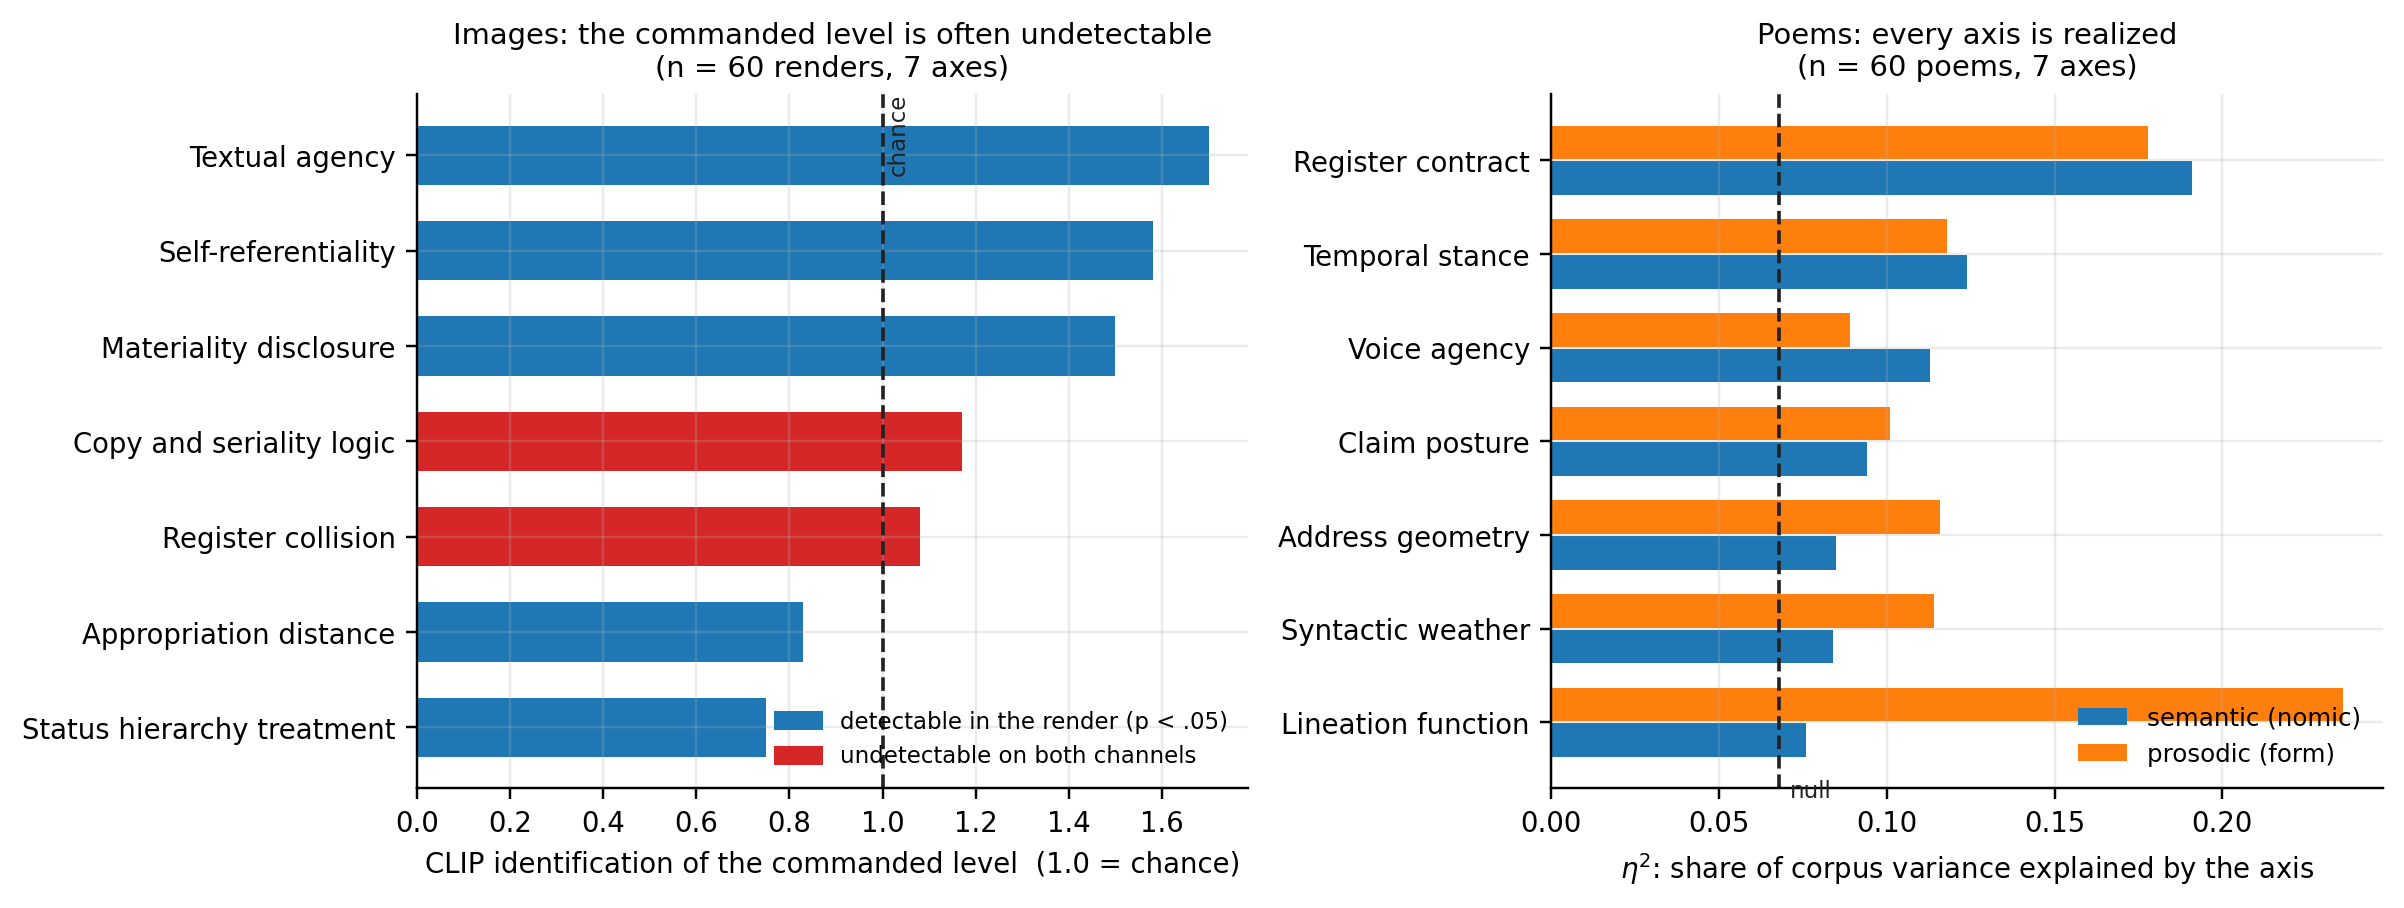
\includegraphics[keepaspectratio,alt={Figure 8. Axis realization measured on the artifact. Left: on 60 max-min renders, three of seven axes identify their commanded level at or below chance, and two are undetectable on both the CLIP and pixel channels. Right: on 60 poems, every axis is realized --- on the semantic channel, the prosodic channel, or both. Dashed lines mark chance and the permutation null.}]{figures/fig17_axis_realization.png}}

\emph{Figure 8. Axis realization measured on the artifact. Left: on 60
max-min renders, three of seven axes identify their commanded level at
or below chance, and two are undetectable on both the CLIP and pixel
channels. Right: on 60 poems, every axis is realized --- on the semantic
channel, the prosodic channel, or both. Dashed lines mark chance and the
permutation null.}

\textbf{The observational audit splits the two domains sharply.} On the
60-render max-min corpus, mean identification is 1.23× chance; three of
seven axes identify their level at or below chance, and only three of
seven move pixel statistics at \emph{p} \textless{} 0.05. The axis the
\emph{attribution} scoring ranked \textbf{first} --- \emph{Copy and
seriality logic} --- is the least realized axis in the corpus on both
channels (\emph{p} = .674 on CLIP, \emph{p} = .920 on pixels), and under
manipulation scoring it ranks last; rank agreement with measured
realization moves from −0.429 to +0.679. This is §5.3\textquotesingle s
inversion in the field rather than in simulation. On the 60-poem pilot
the same audit finds all seven axes realized at \emph{p} \textless{}
0.05 on at least one channel, with effect sizes roughly twice the image
corpora\textquotesingle s.

\textbf{The observational audit is also confounded, and cannot be
de-confounded at these corpus sizes.} It reads a corpus in which the
axes co-vary, so an axis\textquotesingle s apparent effect is entangled
with every axis it travels with; adjusting for that needs a dummy per
level per axis, and with nine to eleven axes at five levels each a
50-poem corpus has fewer rows than columns. The manipulation is
available where the adjustment is not. Holding a base spec fixed, we set
one axis to each of its levels in turn, generate, and read the
displacement --- centring within base so that only variation produced by
\emph{setting} the axis contributes, with a null that shuffles levels
within each base.

\textbf{Poems, by intervention.} Across two independent runs of 440
generations, four axes are realized at \emph{p} \textless{} 0.05 in
both: \emph{Register contract} (ρ = 0.277), \emph{Temporal stance}
(0.240), \emph{{[}form{]} Poem scale} (0.170) and \emph{{[}form{]}
End-rhyme architecture} (0.112), on \textbf{prosody --- a channel the
objective never optimizes}. These are effects in isolation, not in a
live run: the probe removes the avoid-block and the local negatives,
which contribute variance no axis controls, so the same axis accounts
for a smaller share of a running corpus than it does here. What the
probe establishes is the direction the observational audit cannot.
Setting an axis moves the poem. \textbf{Images, by intervention.} The
image pipeline has two stages --- the model that proposed the axes
writes an instruction, and \texttt{gpt-image-1-mini} renders it --- so
the same manipulation can be read on both sides of the handoff. Over all
eleven axes at three bases and five levels, nine of eleven axes are
realized in the \textbf{written instruction} at \emph{p} \textless{}
0.05 (mean ρ = 0.148), against four of eleven in the \textbf{render}
(mean ρ = 0.096); ten of the eleven attenuate, a mean loss of 35\% of
the text-side effect (Wilcoxon signed-rank \emph{p} = .005). The
conditioning is there, in the prompt, and measurable; what fails is its
survival through a generator that never saw the axis set. The companion
paper on proxy embeddings takes that seam as its subject (its §6): it
separates the renderer\textquotesingle s loss from the
instrument\textquotesingle s, since the four perceptual axes attenuate
most in CLIP and are exactly the axes CLIP is least equipped to
register, and it draws the consequence for the modality-agnostic claim
--- it holds for the calculus, which needs only an embedding, and not
for the conditioning, which needs a generator that reads the language
the axes are written in.

\subsubsection{8.2 Expansion: naming what a corpus never
varies}\label{82-expansion-naming-what-a-corpus-never-varies}

Reading the artifacts says the same thing the statistics do, and says it
faster. Eight max-min renders spaced evenly through a sixty-item run
contain four instances of one conceptual gag --- ironic text-in-image
--- and are otherwise uniformly frontal, centred, flat-depth, evenly lit
and saturated. Absent from all eight: photography as a medium,
monochrome or restricted tonal range, shallow depth of field,
directional or low-key lighting, atmospheric or linear perspective,
off-centre composition, and any viewpoint other than eye-level. The
poems fail the same way along a different family: every one of sixty is
roughly fifteen lines of mid-length free verse spoken by a lyric
\emph{I} in one elegiac register, with coefficients of variation of 0.08
on lexical richness, 0.16 on line count and 0.26 on syllables per line.
\emph{Lineation function} is the only formal axis, has the
\textbf{largest} prosodic effect of any axis (η² = 0.236), and still
moves line length by only a quarter of its own mean --- because all five
of its levels are free-verse variants.

Both are the §5.4 limit seen from two domains, and that the missing
family is \emph{optics} for images and \emph{prosody} for poems is not a
coincidence: in both cases it is the dimension the artifact has and the
axis-proposing prompt does not think to ask about, having been asked for
axes of variation in the abstract rather than in the thing being made.

The expansion step is aimed exactly here, and its proposals are
checkable against that reading. Shown twelve renders and told which axes
already exist, the judge returns \emph{viewpoint and perspective},
\emph{directional lighting}, \emph{shot scale} and \emph{motion and
blur}, with concrete levels for each --- the dimensions the reading
named as missing, recovered independently from the pictures alone. Shown
ten poems, it returns \emph{poem scale} (two lines, 3--8, 9--24,
25--100, 100+ in titled sections) and \emph{prosodic grid} (free verse,
syllabic, accentual, accentual-syllabic, fixed metre with end rhyme).

\textbf{Poems: every form dimension opens.} At matched \emph{n},
coefficient of variation on the features the baseline held nearly
constant, each expanded arm scored against its own token-matched
control, three seeds, 50 poems per arm, both conditions from one
generator at one commit:

{\footnotesize
\begin{longtable}[]{@{}>{\raggedright\arraybackslash}p{\dimexpr 0.4361\linewidth-2\tabcolsep\relax}>{\raggedright\arraybackslash}p{\dimexpr 0.1217\linewidth-2\tabcolsep\relax}>{\raggedright\arraybackslash}p{\dimexpr 0.1315\linewidth-2\tabcolsep\relax}>{\raggedright\arraybackslash}p{\dimexpr 0.1315\linewidth-2\tabcolsep\relax}>{\raggedright\arraybackslash}p{\dimexpr 0.1792\linewidth-2\tabcolsep\relax}@{}}
\toprule\noalign{}
form feature & seed 7 & seed 11 & seed 23 & \textbf{mean} \\
\midrule\noalign{}
\endhead
\bottomrule\noalign{}
\endlastfoot
lines per poem & 11.0× & 12.6× & 3.5× & \textbf{9.0×} \\
mean line length & 1.7× & 4.8× & 1.8× & \textbf{2.8×} \\
syllables per line & 1.6× & 5.3× & 1.7× & \textbf{2.8×} \\
syllable-count regularity & 1.5× & 2.2× & 1.9× & \textbf{1.8×} \\
rhyme density & 1.6× & 1.2× & 1.1× & 1.3× \\
type--token ratio & 1.9× & 0.9× & 1.1× & 1.3× \\
\end{longtable}}

Poem length opens in all three seeds --- the ranges run (2, 115), (1,
300) and (2, 32) against controls of (12, 20), (12, 27) and (14, 22) ---
and the two features tied most directly to line construction rise in all
three. The effect is concentrated there: rhyme density moves 1.1× to
1.6× and the type--token ratio is flat, varying between 0.9× and 1.9×
with no consistent direction. \textbf{The generation budget is not what
opens the range.} Long poems need tokens, so every arm is scored against
a control at the same 2,500-token cap with expansion disabled; that
control writes poems of 12 to 20 lines at a line-count coefficient of
variation of 0.112, against 0.117 for the same generator capped at 700
--- four times the budget, no instruction to use it, and the same length
of poem. What opens the range is being asked for two lines, or for a
hundred. And \textbf{semantic diversity rises alongside form diversity
rather than paying for it}: centered Vendi 38.81 → 40.84 and median NN
distance 0.2393 → 0.2976, a 24\% gain, in the same embedding at the same
matched \emph{n}.

Reading the poems is again the fastest check. The expanded corpus
contains a two-line epigram --- \emph{"Had I filed the silence---no: the
silence filed me. / Under review; we remain---perhaps, I remain."} --- a
sixty-line numbered sequence, a bureaucratic intake report, a poem that
arranges itself spatially on the page, and rhymed metrical quatrains:
\emph{"We thought the road would hold us fast, / We kept our names
inside the rain, / We said the worst had surely passed, / Or so we told
ourselves again."} That is iambic tetrameter in ABAB, and \textbf{it
appears nowhere in the baseline sixty at any budget}, because nothing in
the elicited axis set named metre or rhyme. Which absent family the
judge names first is itself seed-dependent --- scale and a combined
prosodic grid at one seed, metre and rhyme as separate axes at the other
two --- so the effect is better described as \emph{expansion opens the
formal dimensions the axis set omitted} than as a claim about any
particular feature.

\pandocbounded{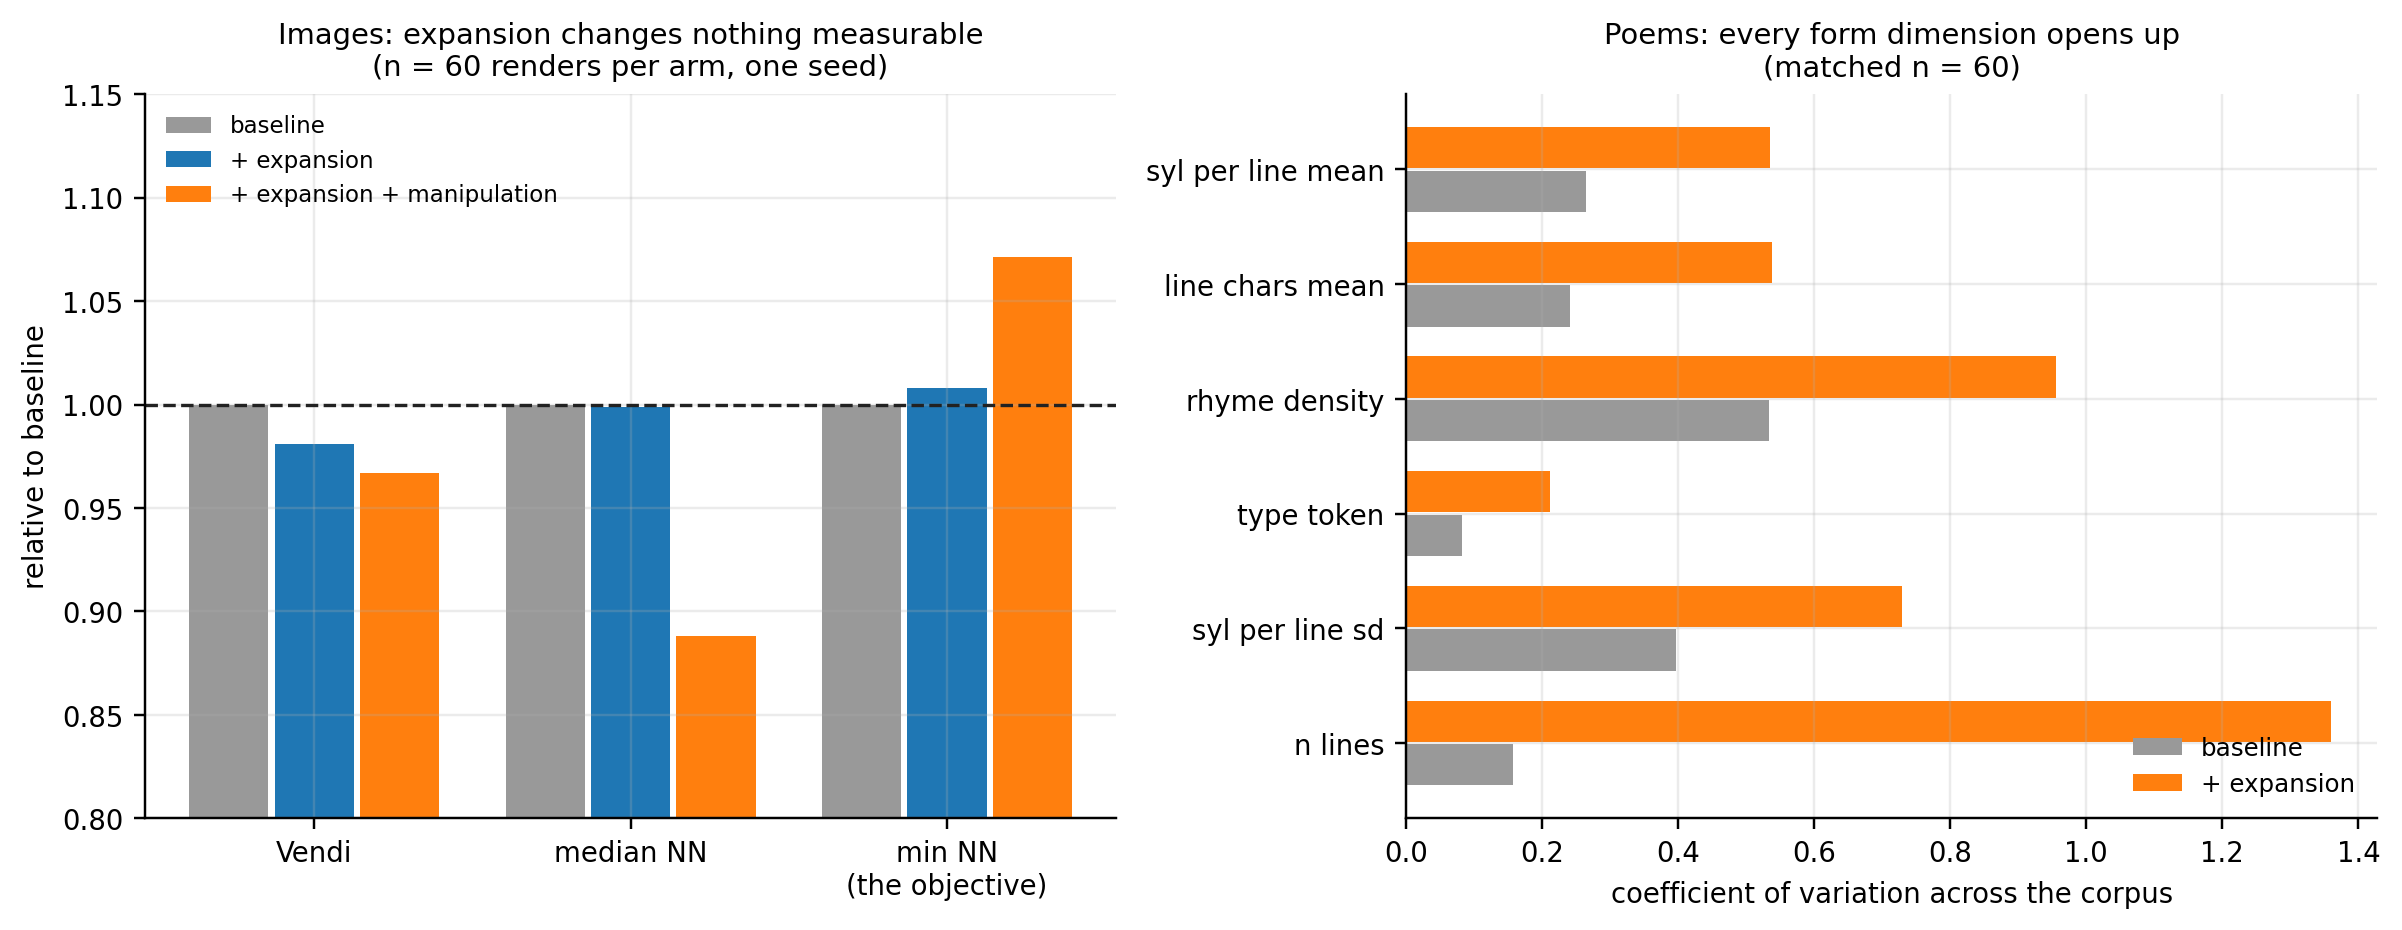
\includegraphics[keepaspectratio,alt={Figure 9. The same expansion mechanism in two domains, at matched budget. Left: three image arms scored relative to the baseline; only min NN distance, the quantity the arm maximizes, improves, and no difference exceeds what one seed can establish. Right: coefficient of variation on poem form features, baseline against expanded --- every dimension the baseline held nearly constant opens up, line count by a factor of nine.}]{figures/fig20_expansion.png}}

\emph{Figure 9. The same expansion mechanism in two domains, at matched
budget. Left: three image arms scored relative to the baseline; only min
NN distance, the quantity the arm maximizes, improves, and no difference
exceeds what one seed can establish. Right: coefficient of variation on
poem form features, baseline against expanded --- every dimension the
baseline held nearly constant opens up, line count by a factor of nine.}

\textbf{Images: no measurable effect, and the reason is a budget nobody
models.} Three arms of sixty renders, one seed, identical seeded axes,
differing only in the mechanism under test, give centered CLIP Vendi
43.81 (baseline) against 42.97 (+expansion) and 42.37 (+expansion,
manipulation-scored); only \texttt{min\ NN\ distance} --- the quantity a
max-min arm actually maximizes --- improves, by 7\%. This is despite the
added perceptual axes being the \emph{best-realized} axes in the run
(mean ρ = 0.036 against 0.016 for the seeded axes) and the renders
visibly acquiring optical modes the baseline never produces: an extreme
macro, a radial-zoom blur, a wide vista with atmospheric depth. At one
seed and \emph{n} = 60 a 3\% Vendi gap is inside run-to-run variation,
so this is a null rather than a ranking.

The explanation is that conditioning on more axes means more contracts
in one prompt, and per-axis obedience falls as that load rises. Four
image arms spanning 7.0 to 11.0 contracts per item, same budget and same
seeded axes:

{\footnotesize
\begin{longtable}[]{@{}>{\raggedright\arraybackslash}p{\dimexpr 0.2835\linewidth-2\tabcolsep\relax}>{\raggedright\arraybackslash}p{\dimexpr 0.1116\linewidth-2\tabcolsep\relax}>{\raggedright\arraybackslash}p{\dimexpr 0.1165\linewidth-2\tabcolsep\relax}>{\raggedright\arraybackslash}p{\dimexpr 0.1064\linewidth-2\tabcolsep\relax}>{\raggedright\arraybackslash}p{\dimexpr 0.1259\linewidth-2\tabcolsep\relax}>{\raggedright\arraybackslash}p{\dimexpr 0.1303\linewidth-2\tabcolsep\relax}>{\raggedright\arraybackslash}p{\dimexpr 0.1259\linewidth-2\tabcolsep\relax}@{}}
\toprule\noalign{}
arm & axes & contracts & per-axis ρ & palette & min NN & Vendi \\
\midrule\noalign{}
\endhead
\bottomrule\noalign{}
\endlastfoot
baseline & 7 & 7.0 & --- & \textbf{0.417} & 0.1540 & \textbf{43.81} \\
+ expansion, manipulation-scored & 10 & 8.7 & 0.0219 & 0.533 & 0.1650 &
42.37 \\
+ expansion & 10 & 9.5 & --- & 0.500 & 0.1552 & 42.97 \\
perceptual axes pre-seeded from item 0 & 11 & 11.0 & 0.0126 &
\textbf{0.667} & 0.1313 & 42.39 \\
\textbf{subset conditioning, 7 of 11} & \textbf{11} & \textbf{7.0} &
0.0167 & 0.500 & \textbf{0.1728} & 43.04 \\
\end{longtable}}

The \emph{palette} column is the fraction of renders sharing a palette
with a nearest neighbour, and it rises with contract load, from 42\% at
seven contracts to 67\% at eleven, and mean realization halves between
the two arms where it is measured. The fourth row is the strongest form
of the expansion test --- the four perceptual axes in force for every
item rather than arriving mid-run, so each conditions 100\% of the
corpus instead of 7\% to 80\% --- and it is the worst arm on every
structural measure. \textbf{An axis added late is diluted by the items
generated before it; an axis added early dilutes every other axis in the
prompt.} There is a contract budget here, and past roughly seven
simultaneous contracts the marginal image axis costs more in compliance
than it returns in reach.

The budget belongs to this conditioning interface rather than to
conditioning in general, and the boundary is informative. The
interventional probe of §8.1, run at seven contracts and at eleven,
finds per-axis obedience \textbf{flat} in the load: across three runs
the mean difference between loads is +0.002, −0.036 and +0.044, changing
sign and swamped by its own spread. An image prompt carries contracts,
mined attractors, structural bans and an overused-word list into a
generator that never saw the axis set; a poem prompt carries contracts
into the model that proposed them. Where the conditioning does not cross
that seam, seven contracts and eleven are equally well honoured.

\textbf{The budget binds the prompt, not the lattice}, and nothing
requires every axis to appear in every spec. Drawing seven contracts per
item from the full eleven-axis set, least-used-axis-first so each axis
accumulates equal usage across the run, keeps the
corpus\textquotesingle s reach while holding prompt load where
compliance is highest. Against the pre-seeded arm --- the same eleven
axes, four fewer contracts --- min nearest-neighbour distance rises
31.6\%, per-axis realization 33\%, and palette sharing falls a quarter;
against the baseline, at the same prompt load but drawing from a lattice
1,300 times larger, min NN is 12.2\% higher, the best value of any arm
here. Centered Vendi and palette sharing sit slightly below baseline, so
this is a gain on the objective rather than a sweep, and at one seed per
arm on the noisiest statistic in this work the magnitude should be read
as approximate. What is not approximate is the design point it makes
concrete: \textbf{the lattice describes what the corpus can reach and
the spec describes what one prompt must carry, and holding the second
fixed while enlarging the first is what lets expansion pay.}

\subsubsection{8.3 Completeness: enumerate the whole space, or the
concentration
moves}\label{83-completeness-enumerate-the-whole-space-or-the-concentration-moves}

Expansion answers \emph{what is missing}, which is the right question
when the missing family is unknown. It does not answer \emph{what must
be covered}. Where a target partition is specified in advance, the
distinction decides whether an intervention helps or backfires, and
following it to its end produces the most transferable rule in this
paper.

An exam item bank is built to a \textbf{blueprint} --- content area
crossed with cognitive level --- so unlike optics or prosody it has a
target partition specified in advance, and coverage of that partition is
what a psychometrician grades. The elicited axes span none of it: all
seven describe item architecture, and the elicitation could not have
proposed otherwise, since it asks for axes of item-design variation and
excludes topic lists. The consequence is visible on the page --- three
items drawn at random are all cloud backup and availability-zone
problems --- and in the corpus, where one blueprint area takes 35\% of
items. Naming breadth in the generation prompt does not help; that
prompt already names architecture, storage, networking, security, cost
and reliability.

Expansion behaves exactly as it does elsewhere and does not fix it.
Shown twelve items, the judge recovers three content dimensions the bank
barely varies --- deployment and locality model, service abstraction
level, data modality --- and they are real dimensions, recovered from
the artifacts alone. Conditioning on them makes the bank
\textbf{lumpier}: under a judge that classifies each item into one
blueprint area, blind to arm, the dominant area\textquotesingle s share
\emph{rises} from 35\% to 47\% and normalized entropy falls from 0.700
to 0.645. The three axes are content-\emph{adjacent} rather than
blueprint-\emph{aligned}: "streaming, analytical, time-series data" is a
genuine axis of variation, and it drives items into one area rather than
across ten.

A single axis whose levels \emph{are} blueprint areas does spread it,
and how much depends on whether it names all of them.

\pandocbounded{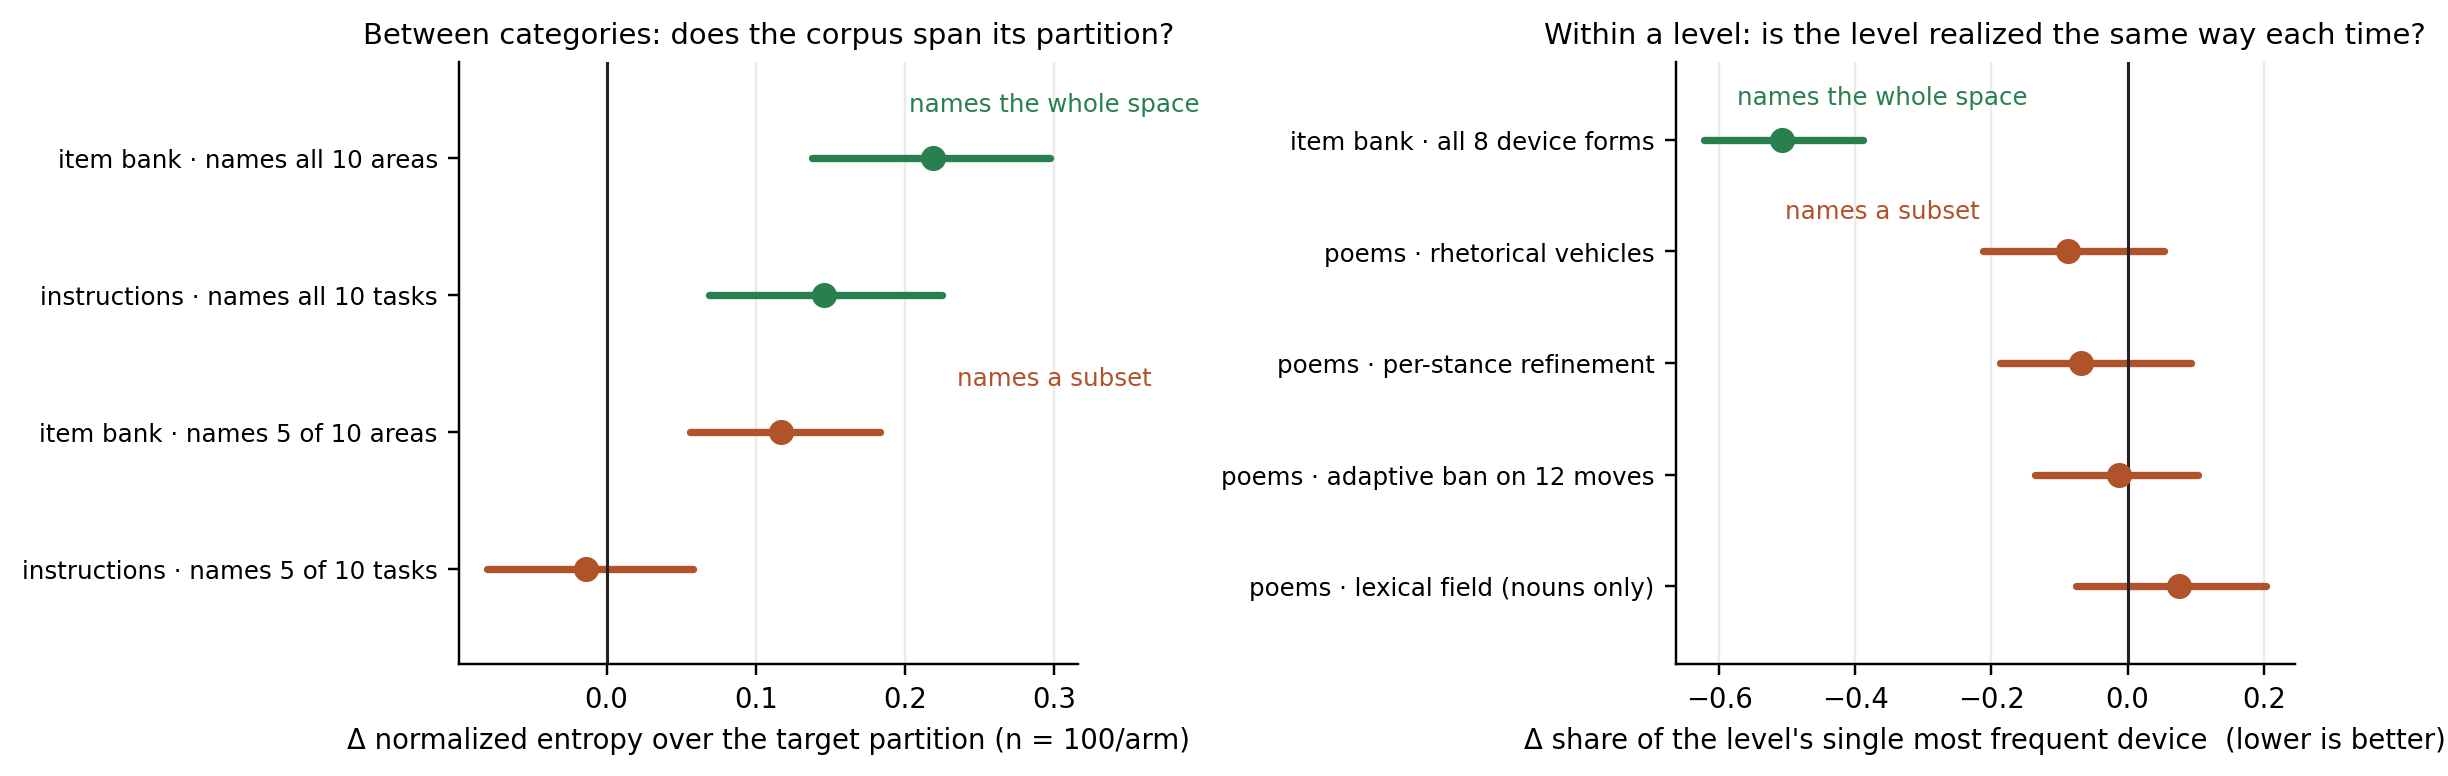
\includegraphics[keepaspectratio,alt={Figure 10. The completeness rule, nine controlled comparisons with blind judges. Left: axes that enumerate a target partition, scored on normalized entropy over that partition (n = 100 per arm, bootstrap 95\% CI). Naming half a partition helps a corpus that is failing to span it and does nothing to one that already spans; naming all of it helps both. Right: axes that enumerate the ways a single level can be realized. The item-bank row is scored by a blind judge on the share of items using the dominant device form; the four poem rows are scored lexically, on the share of each Claim posture level\textquotesingle s poems using that level\textquotesingle s single most frequent non-echo word (n = 80--90 per arm). Enumerating every device form of one construct removes half the concentration; every intervention that names only part of the realization space moves it somewhere else instead.}]{figures/fig23_completeness.png}}

\emph{Figure 10. The completeness rule, nine controlled comparisons with
blind judges. Left: axes that enumerate a target partition, scored on
normalized entropy over that partition (n = 100 per arm, bootstrap 95\%
CI). Naming half a partition helps a corpus that is failing to span it
and does nothing to one that already spans; naming all of it helps both.
Right: axes that enumerate the ways a single level can be realized. The
item-bank row is scored by a blind judge on the share of items using the
dominant device form; the four poem rows are scored lexically, on the
share of each Claim posture level\textquotesingle s poems using that
level\textquotesingle s single most frequent non-echo word (n = 80--90
per arm). Enumerating every device form of one construct removes half
the concentration; every intervention that names only part of the
realization space moves it somewhere else instead.}

An axis naming the \textbf{five underused} areas takes the item
bank\textquotesingle s normalized entropy from 0.700 to 0.816 (+0.117,
95\% CI {[}+0.056, +0.183{]}), the dominant area\textquotesingle s share
from 35\% to 19\%, and the Gini coefficient over areas from 0.606 to
0.410; the three arms\textquotesingle{} distributions differ at χ²(18) =
162.6, \emph{p} = 3 × 10\(^{-25}\). An axis naming \textbf{all ten}
takes it from seven areas to ten and from 0.700 to 0.926 (+0.219,
{[}+0.138, +0.297{]}) --- nearly double.

\textbf{Instructions show why the slice is the weaker instrument.} Their
partition, the taxonomy of what a user asks an assistant to do, is
already spanned by axes describing a request\textquotesingle s
\emph{shape}: six such axes alone reach nine of ten task categories at
entropy 0.811, flatter than the item bank managed with any axis. Adding
an axis naming five underused categories moves an enormous amount of
probability mass --- those five rise from 14\% of the corpus to 81\% ---
and changes total spread not at all (−0.014, {[}−0.080, +0.058{]}),
because the five it does not name are driven out: \emph{decide} from 27
instructions to none, \emph{plan} from 23 to one. An axis enumerating
\textbf{every} category has no unnamed half to trade away, and level
balancing then commands each equally often: entropy 0.811 → 0.959
(+0.146, {[}+0.069, +0.225{]}), all ten categories reached, the largest
taking 25\%. So the prescription is unconditional and needs no prior
audit of where a corpus is thin --- \textbf{where a partition must be
covered, an axis should name all of it} --- and a slice is worth
reaching for only when the goal is to \emph{move} a corpus toward
particular categories rather than to spread it.

\textbf{The same rule holds one level down, and there it exposes a
defect no realization audit can see.} Every audit in §8.1 asks whether a
commanded level \emph{moves} the artifact, and every one computes that
\emph{between} levels. A collapse \emph{within} a level is invisible to
all of them. The psychometric bank shows one. Its
\texttt{Irrelevant-information\ treatment} axis is plainly obeyed ---
items told to carry no irrelevant detail use a colour word 7\% of the
time, items told to carry some use one 52\% to 62\% of the time --- and
yet half of the 1,999-item corpus contains a colour word, because the
red herring is nearly always a coloured card, a star, a printed dot.
Generating afresh reproduces it: under a judge that names the
\emph{form} the irrelevant detail takes, blind to arm, 76\% of items use
a physical-appearance detail and two of eight available forms never
appear, for a normalized device entropy of 0.425 --- far below the
between-category spread of any corpus measured here. This is not
cosmetic. Irrelevant information functions only while the examinee
cannot recognize it by its form; a bank whose red herring is always a
colour sentence teaches candidates to skip colour sentences, and the
distractor stops measuring anything.

The remedy is the same prescription applied inside a level: an axis
enumerating the forms a red herring can take, rather than trusting a
level description to vary its own realization. It takes device entropy
from 0.425 to 0.933 (+0.504, {[}+0.385, +0.626{]}), the dominant form
from 76\% to 24\% (−0.507, {[}−0.622, −0.389{]}), and all eight forms
into use, \textbf{while both arms keep the contract the axis actually
specifies}: in each, 100\% of items still carry detail whose removal
would not change the answer. \textbf{Realization therefore has to be
audited twice --- once to establish that a level moves the artifact, and
once to establish that it does not move it the same way every time.}

The defect is general and the poem corpora carry it more heavily.
Scoring each level by the share of its items using its single most
frequent non-echo content word, poems average 0.533 against 0.412 for
the psychometric bank, with a worst level at 0.811. \emph{Claim posture:
ritual pronouncement} is realized through one liturgical formula --- "By
ash, by antenna, by the names", "By the gathered breath", "By salt and
smoke, I seal this house" --- drawing on a fixed stock of ash, salt,
bells and thresholds across independently generated poems;
\emph{Syntactic weather: nested subordinate clauses} reaches for
\emph{because} in 79\% of its items, and \emph{Register contract:
ceremonial elevation} for \emph{silence} in 72\%. The measure has one
limit worth stating: it cannot distinguish a stereotyped device from a
word the level entails, and \emph{dialogue with conflicting claims}
scoring 0.73 on \emph{says} is the latter, which is why the levels above
were read rather than only counted.

\textbf{Three attempts to transfer the remedy fail in the same shape,
and that is what identifies the rule.} A red herring\textquotesingle s
forms are a closed list; a poetic stance can be delivered by any
rhetorical means. Enumerating \emph{vehicles} instead --- an imperative,
an unanswered question, a negation, a bare object, a reported speech
act, a conditional, an inventory, a self-correction --- is orthogonal to
which stance is carried and composes with every stance axis. It lowers
device share on \textbf{all seven} poem axes at once, 0.618 → 0.570 (7
of 7, one-sided sign test \emph{p} = .008; the aggregate difference is
−0.048, {[}−0.101, +0.012{]}) while the commanded posture is still
exhibited in 96\% of poems against 95\% without it. But the \emph{size}
is the point of contrast: an axis enumerating the realization space of a
specific construct moved an item bank\textquotesingle s dominant form
from 76\% to 24\%, where a general vehicle axis moves poems by 0.04 and
leaves \emph{ritual pronouncement} reaching for \emph{let} in 69\% of
its poems, down from 88\%.

Making the poem axis construct-specific does not close the gap. Refining
each posture into five ways \emph{that} stance is performed --- ritual
pronouncement into invocation, blessing, oath, anathema, consecration
--- gives the largest single-level improvement of any arm (\emph{let}
falls to 56\%) and the highest contract adherence (99\%), and does not
lower device share overall (0.595 against a 0.662 baseline, −0.068
{[}−0.188, +0.093{]}) because \emph{name} becomes the dominant word in
three of five levels. Nor does making the ban adaptive: rebuilding it
every batch from a judge\textquotesingle s reading of the rhetorical
\emph{moves} the corpus has just started overusing --- the register the
defect actually lives in --- leaves device share at 0.650 (−0.012,
{[}−0.136, +0.104{]}), with \emph{let} falling from 88\% to 69\% for
ritual pronouncement and \emph{through} arriving at 69\%. Twelve banned
moves is still a subset.

The clearest case is the one that makes the concentration
\textbf{worse}. Commanding the poem\textquotesingle s concrete nouns
from one of eight lexical fields is obeyed almost perfectly --- the
commanded field\textquotesingle s vocabulary appears in 98\% of poems
and is the dominant field in 94\%, against a chance rate of 12.5\% ---
and device share nevertheless \emph{rises}, 0.662 → 0.738 (+0.076,
{[}−0.076, +0.204{]}), with the posture contract holding at 96\% and
craft unharmed. The words carrying the new concentration are the ones
the axis left free: \emph{confess} in 81\% of confessional poems,
\emph{mine} in 88\% of refusals, \emph{beneath} in 75\% of flat
assertions. \textbf{Constraining the nouns concentrated the verbs and
pronouns.}

The rule that explains all seven comparisons without appealing to domain
is therefore about \emph{completeness}:

\begin{quote}
\textbf{An intervention that enumerates a proper subset of the space a
measure is defined over displaces concentration into the complement;
only enumerating the whole space reduces it.}
\end{quote}

{\footnotesize
\begin{longtable}[]{@{}>{\raggedright\arraybackslash}p{\dimexpr 0.4273\linewidth-2\tabcolsep\relax}>{\raggedright\arraybackslash}p{\dimexpr 0.1955\linewidth-2\tabcolsep\relax}>{\raggedright\arraybackslash}p{\dimexpr 0.3772\linewidth-2\tabcolsep\relax}@{}}
\toprule\noalign{}
intervention & enumerates & effect on the measured concentration \\
\midrule\noalign{}
\endhead
\bottomrule\noalign{}
\endlastfoot
5 of 10 task categories & subset & unnamed half 86\% → 19\%; total
spread flat \\
all 10 task categories & whole & spread up in a lumpy corpus
\textbf{and} a flat one \\
all 8 device forms of one construct & whole & dominant form 76\% →
24\% \\
rhetorical vehicles (partial lexical control) & subset & −0.04; mass
moves to a new word \\
per-stance device refinement & subset & flat; \emph{name} becomes
dominant in 3 of 5 levels \\
adaptive ban on 12 rhetorical moves & subset & flat; \emph{let} →
\emph{through} \\
lexical field over nouns & subset & obeyed 94\%; mass moves to verbs and
pronouns \\
ban on the 8 most overused words (images) & subset & +0.089;
\emph{light} → \emph{illumination} \\
ban on the 8 most overused words (poems) & subset & +0.112; \emph{let} →
\emph{beneath}, \emph{answer} → \emph{perhaps} \\
mined attractors, stated as prose & not an enumeration & −0.136, the
largest reduction measured \\
\end{longtable}}

One measurement keeps this from being read as conservation. On
whole-vocabulary mean pairwise word overlap between poems sharing a
posture, the lexical arm has the \textbf{lowest} overall repetition of
any arm (0.0387, {[}0.0363, 0.0412{]} against the
baseline\textquotesingle s 0.0452) at the same time as one word becomes
more dominant within it. Both are true --- the field axis spreads the
nouns across the corpus while the posture\textquotesingle s stock verb
tightens --- and total overlap varies across arms by 14\%, so repetition
is not a fixed budget that conditioning merely shuffles. What
conditioning reliably does is leave concentration wherever the axis set
does not reach. That is the argument for auditing realization in a
channel the objective never optimizes, for measuring it more than one
way, and for reading the artifacts rather than only the scores.

The rule reaches the pipeline\textquotesingle s own machinery, where the
two blocks that stand against concentration pull in opposite directions.
Image instructions written from the contracts alone are dominated by
\emph{mixed-media} on nine of eleven axes, a within-level concentration
of 0.564. Adding the hard block --- the structural bans together with a
list of the corpus\textquotesingle s eight most overused words ---
raises that to 0.653, and adding both blocks raises it further; adding
the mined-attractor block alone lowers it to 0.427 and leaves no
dominant device behind. All four arms wrote 110 of 110 instructions, and
every device is scored with the vocabulary of each arm\textquotesingle s
own prompt blocks excluded, so no arm is credited for repeating its
instructions back.

What replaces what shows the mechanism at word granularity. The hard
block bans \emph{light}; \emph{illumination} becomes the dominant device
on fifty of the level-slots measured. Banning a word leaves the concept,
and the generator reaches for its nearest synonym. A prohibition names a
subset by construction --- that is what a prohibition \emph{is} --- so
it relocates concentration rather than reducing it, exactly as an axis
does. The attractor block is the one mechanism measured here that does
not: it describes a \emph{tendency} in prose instead of enumerating
tokens, and so offers no complement for the mass to move into.

The effect replicates in poems, where the substitutions are legible one
by one. Banning the eight words the corpus most overuses ---
\emph{still, hand, name, record, rain, let, say, silence}, seven of them
already the dominant device of some level --- raises device share from
0.525 to 0.637 (+0.112, 95\% CI {[}+0.016, +0.180{]}) when both arms are
scored on the vocabulary available to both, and every level rises:
\emph{record} gives way to \emph{because}, \emph{answer} to
\emph{perhaps}, \emph{mine} to \emph{cannot}, \emph{let} to
\emph{beneath}. The commanded posture survives in 98\% of poems, so this
is displacement rather than a broken contract, but craft falls to 5.97
from the 6.5 to 6.7 of the other arms. Prohibition at the token level
costs quality and buys concentration, in both domains where it has been
measured.

Taken together the interventions grade by what they name rather than by
domain: banning tokens makes concentration worse, banning tendencies
leaves it flat, and enumerating a whole space is the only thing that
reduces it.

\subsubsection{\texorpdfstring{8.4 What best-of-\emph{K} buys depends on
what the selector
optimizes}{8.4 What best-of-K buys depends on what the selector optimizes}}\label{84-what-best-of-k-buys-depends-on-what-the-selector-optimizes}

§4.2 shows that best-of-\emph{K} oversampling improves the expected
min-gap only as \emph{K}\(^{1/m}\), and that result assumes selection
\emph{on the gap}. Our own loop does not select that way: it keeps the
candidate maximizing 0.40·craft + 0.35·orthogonality +
0.25·min-distance, a blend in which the quantity the corpus is scored on
carries the smallest weight. The distinction is measurable, and it
matters more than the weights suggest. Poem arms of 50 items at \emph{K}
= 6, three seeds, changing only the selection rule:

{\footnotesize
\begin{longtable}[]{@{}>{\raggedright\arraybackslash}p{\dimexpr 0.2545\linewidth-2\tabcolsep\relax}>{\raggedright\arraybackslash}p{\dimexpr 0.1232\linewidth-2\tabcolsep\relax}>{\raggedright\arraybackslash}p{\dimexpr 0.1273\linewidth-2\tabcolsep\relax}>{\raggedright\arraybackslash}p{\dimexpr 0.1423\linewidth-2\tabcolsep\relax}>{\raggedright\arraybackslash}p{\dimexpr 0.1232\linewidth-2\tabcolsep\relax}>{\raggedright\arraybackslash}p{\dimexpr 0.1147\linewidth-2\tabcolsep\relax}>{\raggedright\arraybackslash}p{\dimexpr 0.1147\linewidth-2\tabcolsep\relax}@{}}
\toprule\noalign{}
seed & min NN, blend & min NN, gap-only & 5th-pctile NN, blend &
gap-only & craft, blend & gap-only \\
\midrule\noalign{}
\endhead
\bottomrule\noalign{}
\endlastfoot
7 & 0.1910 & 0.2510 & 0.2111 & 0.2538 & 8.54 & 8.17 \\
11 & 0.1920 & 0.2168 & 0.1984 & 0.2413 & 8.55 & 8.16 \\
23 & 0.2377 & 0.2788 & 0.2427 & 0.2796 & 8.47 & 8.26 \\
\textbf{mean} & \textbf{0.2069} & \textbf{0.2489} & \textbf{0.2174} &
\textbf{0.2582} & \textbf{8.52} & \textbf{8.20} \\
\end{longtable}}

Selecting on the gap alone raises the minimum nearest-neighbour distance
in \textbf{3 of 3 seeds}, by \textbf{+20.3\%} on the means (range
+12.9\% to +31.5\%; paired \emph{t}(2) = 4.13, \emph{p} = 0.054), and
the fifth percentile by 18.8\%. It costs 0.32 of a craft point on a
ten-point scale, and the cost replicates more tightly than the benefit
--- 8.52 ± 0.04 against 8.20 ± 0.04 --- which is what a utility term
being removed should look like. The effect also explains a sweep that is
otherwise puzzling: under the blended selector min NN is \textbf{not
monotone in \emph{K}} (0.1828 at \emph{K} = 1, 0.2148 at 3, 0.1910 at
6), and under the gap-only selector it is (0.2278 at 3, 0.2510 at 6).
Additional candidates do buy minimum gap, but only for a selector that
spends them on it; the blend spends them on craft and bulk spread, both
of which rise monotonically in \emph{K} under either rule.

The practical statement is narrow and easy to get wrong: \textbf{a
corpus scored on min-gap and selected on a quality-weighted blend is
being oversampled for something other than what it is scored on.} The
\emph{K}\(^{1/m}\) ceiling is real, and a system can fail to reach even
that ceiling by pointing its selector elsewhere. Three seeds at \emph{n}
= 50 is a small replication and the effect size varies by a factor of
two and a half across them; the direction is consistent and the
magnitude approximate.

The same question at the \emph{render} has a sharper answer, because the
two channels have very different effective dimensions. Best-of-\emph{K}
on the written candidate happens before the handoff and §8.1 locates the
loss after it, so we also ran \emph{K} = 3 renders behind each of 60
fixed instructions and kept the render maximizing min distance to the
accepted set --- once in CLIP, once in optical statistics, over the same
candidates. Selecting on optics raises pixel min NN from 1.039 to 1.292
(1.24×) and the fifth-percentile NN by 0.336 (paired subsample, 95\% CI
{[}+0.128, +0.488{]}), \textbf{and costs nothing in the channel the
method optimizes}: CLIP min NN moves by −0.001 with the interval
{[}−0.029, +0.033{]} tight around zero. Selecting on CLIP raises CLIP
min NN by 0.040 ({[}+0.025, +0.071{]}) and moves optics not at all
detectably. Both gains lie on the \emph{K}\(^{1/m}\) curve --- 1.24× at
\emph{K} = 3 implies \emph{m} ≈ 4.4, and 1.04× implies \emph{m} ≈ 17 ---
so render-side selection is oversampling rather than a new mechanism.
What the dimensions add is an allocation rule: oversampling buys far
more in a low-dimensional channel than in a high-dimensional one, and
\textbf{if a pipeline is going to pay for extra renders, it should
select them on the channel the objective cannot see.}

\subsection{9. Limitations}\label{9-limitations}

\begin{itemize}
\tightlist
\item
  \textbf{One embedding oracle.} All geometry is
  \texttt{nomic-embed-text} geometry with cosine distance, on both
  objectives. Whether "diverse" or "covered" under one embedder
  transfers to another is the subject of the companion paper on proxy
  embeddings, which measures text-to-CLIP correlations on rendered
  outputs of only \emph{r} = 0.167 to 0.421 and shows per-arm audio
  diversity verdicts flipping between embedders, and which shows the
  \emph{ranking} of methods surviving four independent representations.
  For any domain with a downstream rendering step the objective should
  be defined in the space the artifact actually occupies. Here it was
  not.
\end{itemize}

\subsection{10. Conclusion}\label{10-conclusion}

No measure here is limited by its optimizer. What determines whether a
corpus can keep growing without collapsing into paraphrase, and whether
it can blanket the space it is drawn from, is the dimension of the
generator\textquotesingle s conditional support relative to the manifold
it lives in. Saturation arrives at rate \emph{n}\(^{-1/m}\) rather than
\emph{n}\(^{-1/d}\), a single prompt covers an ε\(^{d-m}\) fraction of
what the model could write, and only transverse prompt motion raises the
ceiling. Everything else buys a constant factor against an asymptotic
problem.

Given an embedding oracle and no inverse, the system cannot compute its
way to the next item; it can only choose what to condition on. Recursive
Axis Conditioning is our answer, and it works: first of twelve corpora
against released instruction sets at a twentieth of the budget, an exam
bank with no enemy pair at a judged radius where naive prompting yields
15\% of nominal capacity, and separation from every baseline in three
artifact domains measured on channels the loop never optimizes. Its most
valuable output is the refine signal --- the moment the scoring reports
that nothing available is transverse any more is the moment the horizon
has been reached, and the only remaining move is to ask the generator to
subdivide its own vocabulary of variation.

Three lessons transfer past the method.

\textbf{Name the measure, because the two classes are not one problem.}
Greedy \emph{k}-center wins min-gap in both domains and finishes last on
coverage; orthogonalized conditioning, load-bearing under max-min,
scores below doing nothing at all under coverage. Pointing the loop
changes exactly two things, how an axis is scored and how a candidate is
chosen, and those two are enough to invert which method looks best. A
corpus is diverse \emph{with respect to} an objective.

\textbf{Score your control variables by manipulation, not by
attribution.} Level vectors read off a corpus in which every axis varies
at once are marginal means, and because an effective axis fills the
corpus with variance along its own direction while transversality
credits variation lying outside the occupied span, the resulting score
penalizes an axis in proportion to how well it works. On data where the
answer is fixed by construction the observational form ranks the inert
axis first in most runs; partial effects and a null-corrected
realization factor recover the true order. The lesson generalizes to any
system that scores its own control variables against its own outputs.

\textbf{Name the whole space, or the repetition moves.} Conditioning
does not so much remove a corpus\textquotesingle s tendency to repeat
itself as relocate it into whatever the axis set does not name. An axis
over half a task partition drove the unnamed half from 86\% of a corpus
to 19\% and left total spread unchanged; an axis over all of it raised
spread in a lumpy corpus and a flat one. An axis over every form a red
herring can take moved an item bank\textquotesingle s dominant device
from 76\% to 24\%; axes over part of a poem\textquotesingle s
realization space moved it by 0.04, or made it worse while being obeyed
94\% of the time. The corollary is a practice, not a theorem:
realization has to be audited twice, once between levels and once within
one, because a level that is obeyed every time and performed identically
every time passes every check in the literature.

Two things bound all of it, and both are measured in the companion paper
on proxy embeddings. The first is a seam: conditioning reaches the
written instruction at mean ρ = 0.148 and the render at 0.096, so a
third of its grip is lost exactly where one model\textquotesingle s
language becomes another model\textquotesingle s input, and where that
seam exists axis realization has to be measured rather than assumed. The
second is sharper. Ninety percent of our generated exam
bank\textquotesingle s answer keys sit in option position A --- a bank
an examinee can score 90\% on without reading a stem --- and not one
measure in this paper detects it, because key position carries no
semantic content for an embedding to encode. A diversity objective
defined over an embedding cannot see any property the embedding does not
encode, including the ones that decide whether the artifact is usable at
all.

Which is the argument for the practice we ended up recommending, and it
is short. Count your duplicates before computing anything else. Report
the literal and the latent separately, and name the denominator. Check
that the knobs you are turning are connected to anything, by
intervention rather than by correlation. Measure at the level of the
artifact you are shipping, and audit in at least one channel your
objective cannot see --- it is where we found both our strongest result
and our largest undetected defect. And read the output, because a corpus
can be diverse along every dimension you thought to name and uniform
along the one you did not.

\end{document}
